\documentclass[a4paper]{article}
\usepackage[ngerman]{babel}
\usepackage[utf8]{inputenc}
\usepackage{multicol}
\usepackage{calc}
\usepackage{ifthen}
\usepackage[landscape]{geometry}
\usepackage{amsmath,amsthm,amsfonts,amssymb}
\usepackage{color,graphicx,overpic}
\usepackage{xcolor, listings}
\usepackage[compact]{titlesec} %less space for headers
\usepackage{mdwlist} %less space for lists
\usepackage{pdflscape}
\usepackage{verbatim}
\usepackage[most]{tcolorbox}
\usepackage[hidelinks,pdfencoding=auto]{hyperref}
\usepackage{bussproofs}
\usepackage{fancyhdr}
\usepackage{lastpage}
\pagestyle{fancy}
\fancyhf{}
\fancyhead[L]{Advanced Operating Systems}
\fancyfoot[L]{\thepage/\pageref{LastPage}}
\renewcommand{\headrulewidth}{0pt} %obere Trennlinie
\renewcommand{\footrulewidth}{0pt} %untere Trennlinie

\usepackage{pifont}
\newcommand{\cmark}{\ding{51}}
\newcommand{\xmark}{\ding{55}}

\pdfinfo{
 /Title (Advanced Operating Systems - Cheatsheet)
 /Creator (TeX)
 /Producer (pdfTeX 1.40.0)
 /Author (Robert Jeutter)
 /Subject ()
}

%%% Code Listings
\definecolor{codegreen}{rgb}{0,0.6,0}
\definecolor{codegray}{rgb}{0.5,0.5,0.5}
\definecolor{codepurple}{rgb}{0.58,0,0.82}
\definecolor{backcolour}{rgb}{0.95,0.95,0.92}
\lstdefinestyle{mystyle}{
 backgroundcolor=\color{backcolour}, 
 commentstyle=\color{codegreen},
 keywordstyle=\color{magenta},
 numberstyle=\tiny\color{codegray},
 stringstyle=\color{codepurple},
 basicstyle=\ttfamily,
 breakatwhitespace=false, 
}
\lstset{style=mystyle, upquote=true}

%textmarker style from colorbox doc
\tcbset{textmarker/.style={%
 enhanced,
 parbox=false,boxrule=0mm,boxsep=0mm,arc=0mm,
 outer arc=0mm,left=2mm,right=2mm,top=3pt,bottom=3pt,
 toptitle=1mm,bottomtitle=1mm,oversize}}

% define new colorboxes
\newtcolorbox{hintBox}{textmarker,
 borderline west={6pt}{0pt}{yellow},
 colback=yellow!10!white}
\newtcolorbox{importantBox}{textmarker,
 borderline west={6pt}{0pt}{red},
 colback=red!10!white}
\newtcolorbox{noteBox}{textmarker,
 borderline west={3pt}{0pt}{green},
 colback=green!10!white}

% define commands for easy access
\renewcommand{\note}[2]{\begin{noteBox} \textbf{#1} #2 \end{noteBox}}
\newcommand{\warning}[1]{\begin{hintBox} \textbf{Warning:} #1 \end{hintBox}}
\newcommand{\important}[1]{\begin{importantBox} \textbf{Important:} #1 \end{importantBox}}

% This sets page margins to .5 inch if using letter paper, and to 1cm
% if using A4 paper. (This probably isn't strictly necessary.)
% If using another size paper, use default 1cm margins.
\ifthenelse{\lengthtest { \paperwidth = 11in}}
 { \geometry{top=.5in,left=.5in,right=.5in,bottom=.5in} }
 {\ifthenelse{ \lengthtest{ \paperwidth = 297mm}}
 {\geometry{top=1.3cm,left=1cm,right=1cm,bottom=1.2cm} }
 {\geometry{top=1.3cm,left=1cm,right=1cm,bottom=1.2cm} }
 }

% Redefine section commands to use less space
\makeatletter
\renewcommand{\section}{\@startsection{section}{1}{0mm}%
 {-1ex plus -.5ex minus -.2ex}%
 {0.5ex plus .2ex}%x
 {\normalfont\large\bfseries}}
\renewcommand{\subsection}{\@startsection{subsection}{2}{0mm}%
 {-1explus -.5ex minus -.2ex}%
 {0.5ex plus .2ex}%
 {\normalfont\normalsize\bfseries}}
\renewcommand{\subsubsection}{\@startsection{subsubsection}{3}{0mm}%
 {-1ex plus -.5ex minus -.2ex}%
 {1ex plus .2ex}%
 {\normalfont\small\bfseries}}
\makeatother

% Don't print section numbers
\setcounter{secnumdepth}{0}

\setlength{\parindent}{0pt}
\setlength{\parskip}{0pt plus 0.5ex} 
% compress space
\setlength\abovedisplayskip{0pt}
\setlength{\parskip}{0pt}
\setlength{\parsep}{0pt}
\setlength{\topskip}{0pt}
\setlength{\topsep}{0pt}
\setlength{\partopsep}{0pt}
\linespread{0.5}
\titlespacing{\section}{0pt}{*0}{*0}
\titlespacing{\subsection}{0pt}{*0}{*0}
\titlespacing{\subsubsection}{0pt}{*0}{*0}

\begin{document}

\raggedright
\begin{multicols}{3}\scriptsize % multicol parameters % These lengths are set only within the two main columns %\setlength{\columnseprule}{0.25pt} \setlength{\premulticols}{1pt} \setlength{\postmulticols}{1pt} \setlength{\multicolsep}{1pt} \setlength{\columnsep}{2pt} 

    \subsection{Funktionale und nichtfunktionale Eigenschaften}
    \begin{itemize*}
        \item Requirements: (nicht-)Funktionale Eigenschaften entstehen durch Erfüllung von (nicht-)funktionalen Anforderungen
        \item funktionale Eigenschaft: was ein Produkt tun soll
        \item nichtfunktionale Eigenschaft (NFE): wie ein Produkt dies tun soll
        \item andere Bezeichnungen NFE: Qualitäten, Quality of Service
    \end{itemize*}

    \subsubsection{Hardwarebasis}
    \begin{itemize*}
        \item Einst: Einprozessor-Systeme
        \item Heute: Mehrprozessor-/hochparallele Systeme
        \item neue Synchronisationsmechanismen erforderlich
        \item[$\rightarrow$] unterschiedliche Hardware und deren Multiplexing
    \end{itemize*}

    \subsubsection{Betriebssystemarchitektur}
    \begin{itemize*}
        \item Einst: Monolithische und Makrokernel-Architekturen
        \item Heute: Mikrokernel(-basierte) Architekturen
        \item Exokernelbasierte Architekturen (Library-Betriebssysteme)
        \item Virtualisierungsarchitekturen
        \item Multikernel-Architekturen
        \item[$\rightarrow$] unterschiedliche Architekturen
    \end{itemize*}

    \subsubsection{Ressourcenverwaltung}
    \begin{itemize*}
        \item Einst: Batch-Betriebssysteme, Stapelverarbeitung (FIFO)
        \item Heute: Echtzeitgarantien für Multimedia und Sicherheit
        \item echtzeitfähige Scheduler, Hauptspeicherverwaltung, Ereignismanagement, Umgang mit Überlast/Prioritätsumkehr ...
        \item[$\rightarrow$] unterschiedliche Ressourcenverwaltung
    \end{itemize*}

    \subsubsection{Betriebssystemabstraktionen}
    \begin{itemize*}
        \item Reservierung von Ressourcen ( $\rightarrow$ eingebettete Systeme)
        \item Realisierung von QoS-Anforderungen ( $\rightarrow$ Multimediasysteme)
        \item Erhöhung der Ausfallsicherheit ( $\rightarrow$ verfügbarkeitskritisch)
        \item Schutz vor Angriffen und Missbrauch ( $\rightarrow$ sicherheitskritisch)
        \item flexiblen und modularen Anpassen des BS ( $\rightarrow$ hochadaptiv)
        \item[$\rightarrow$] höchst diverse Abstraktionen von Hardware
    \end{itemize*}

    \subsubsection{Betriebssysteme als Softwareprodukte}
    \begin{itemize*}
        \item Betriebssystem: endliche Menge von Quellcode
        \item besitzen differenzierte Aufgaben $\rightarrow$ funktionale Eigenschaften
        \item Anforderungen an Nutzung und Pflege $\rightarrow$ Evolutionseigenschaften
        \item können für Betriebssysteme höchst speziell sein
        \item[$\rightarrow$] spezielle Anforderungen an das Softwareprodukt BS
    \end{itemize*}

    Grundlegende funktionale Eigenschaften von BS: Hardware-
    \begin{description*}
        \item[Abstraktion] Ablaufumgebung auf Basis der Hardware bereitstellen
        \item[Multiplexing] Ablaufumgebung zeitlich/logisch getrennt einzelnen Anwendungen zuteilen
        \item[Schutz] gemeinsame Ablaufumgebung gegen Fehler und Manipulation
    \end{description*}

    Nichtfunktionale Eigenschaften (Auswahl) von Betriebssystemen:
    \begin{itemize*}
        \item Laufzeiteigenschaften: zur Laufzeit eines Systems beobachtbar
        \begin{itemize*}
            \item Sparsamkeit und Effizienz
            \item Robustheit, Verfügbarkeit
            \item Sicherheit (Security)
            \item Echtzeitfähigkeit, Adaptivität, Performanz
        \end{itemize*}
        \item Evolutionseigenschaften: charakterisieren (Weiter-) Entwicklung- und Betrieb eines Systems
        \begin{itemize*}
            \item Wartbarkeit, Portierbarkeit
            \item Offenheit, Erweiterbarkeit
        \end{itemize*}
    \end{itemize*}

    \section{Sparsamkeit und Effizienz}
    \subsection{Motivation}
    Sparsamkeit (Arbeitsdefinition): Die Eigenschaft eines Systems, seine
    Funktion mit minimalem Ressourcenverbrauch auszuüben $\rightarrow$ Effizienz bei Nutzung der Ressourcen

    Effizienz: Der Grad, zu welchem ein System oder eine seiner Komponenten
    seine Funktion mit minimalem Ressourcenverbrauch ausübt. (IEEE)

    Beispiele:
    \begin{itemize*}
        \item mobile Geräte: Sparsamkeit mit Energie
        \item Sparsamkeit mit weiteren Ressourcen, z.B. Speicherplatz
        \item Betriebssystem (Kernel + User Space): geringer Speicherbedarf
        \item optimale Speicherverwaltung durch Betriebssystem zur Laufzeit
        \item Baugrößenoptimierung(Platinen-und Peripheriegerätegröße)
        \item Kostenoptimierung(kleine Caches, keine MMU, ...)
        \item massiv reduzierte HW-Schnittstellen (E/A-Geräte, Peripherie)
    \end{itemize*}

    Mobile und eingebettete Systeme (kleine Auswahl)
    \begin{itemize*}
        \item mobile Rechner-Endgeräte
        \item Weltraumfahrt und -erkundung
        \item Automobile
        \item verteilte Sensornetze (WSN)
        \item Chipkarten
        \item Multimedia-und Unterhaltungselektronik
    \end{itemize*}

    \subsection{Energieeffizienz}
    zeitweiliges Abschalten momentan nicht benötigter Ressourcen

    Betriebssystemmechanismen
    \begin{enumerate*}
        \item Dateisystem-E/A: energieeffizientes Festplatten-Prefetching
        \item CPU-Scheduling: energieeffizientes Scheduling
        \item Speicherverwaltung: Lokalitätsoptimierung
        \item Netzwerk: energiebewusstes Routing
        \item Verteiltes Rechnen: temperaturabhängige Lastverteilung
    \end{enumerate*}

    \subsubsection{Energieeffiziente Dateizugriffe}
    HDD/Netzwerkgeräte/... sparen nur bei relativ langer Inaktivität Energie
    \begin{itemize*}
        \item Aufgabe: kurze, intensive Zugriffsmuster $\rightarrow$ lange Inaktivität
        \item HDD-Geräten: Zustände mit absteigendem Energieverbrauch:
        \begin{enumerate*}
            \item Aktiv: einziger Arbeitszustand
            \item Idle: Platte rotiert, Elektronik teilweise abgeschaltet
            \item Standby: Rotation abgeschaltet
            \item Sleep: gesamte restliche Elektronik abgeschaltet
        \end{enumerate*}
        \item ähnliche, noch stärker differenzierte Zustände bei DRAM
        %\item \includegraphics[width=\linewidth]{Assets/AdvancedOperatingSystems-energiezustände-festplatte.png}
        \item durch geringe Verlängerungen des idle - Intervalls kann signifikant der Energieverbrauch reduziert werden
    \end{itemize*}

    \subsubsection{Prefetching-Mechanismus}
    \begin{itemize*}
        \item Prefetching (,,Speichervorgriff'', vorausschauend) \& Caching
        \begin{itemize*}
            \item Standard-Praxis bei moderner Datei-E/A
            \item Voraussetzung: Vorwissen über benötigte Folge von zukünftigen Datenblockreferenzen
            \item Ziel: Performanzverbesserung durch Durchsatzerhöhung und Latenzzeit-Verringerung
            \item Idee: Vorziehen möglichst vieler E/A-Anforderungen an Festplatte + zeitlich gleichmäßige Verteilung verbleibender
            \item Umsetzung: Caching dieser vorausschauend gelesenen Blöcke in ungenutzten PageCache
        \end{itemize*}
        \item[$\rightarrow$] Inaktivität überwiegend sehr kurz $\rightarrow$ Energieeffizienz ...?
        \item Zugriffs-/Festplattenoperationen
        \begin{itemize*}
            \item access(x) ... greife auf Inhalt von Festplattenblock x im PageCache zu
            \item fetch(x) ... hole Block x nach einem access(x) von Festplatte
            \item prefetch(x) ... hole Block x ohne access(x) von Festplatte
        \end{itemize*}
        \item Fetch-on-Demand-Strategie bisher (kein vorausschauendes Lesen)
        \item Traditionelles Prefetching
        \begin{itemize*}
            \item traditionelle Prefetching-Strategie: bestimmt
            \begin{itemize*}
                \item wann Block von der Platte holen (HW aktiv)
                \item welcher Block zu holen ist
                \item welcher Block zu ersetzen ist
            \end{itemize*}
        \end{itemize*}
        \begin{enumerate*}
            \item Optimales Prefetching: Jedes \emph{prefetch} sollte den nächsten Block im Referenzstrom in den Cache bringen, der noch nicht dort ist
            \item Optimales Ersetzen: Bei jedem ersetzenden \emph{prefetch} sollte der Block überschrieben werden, der am spätesten in der Zukunft wieder benötigt wird
            \item ,,Richte keinen Schaden an'': Überschreibe niemals Block A um Block B zu holen, wenn A vor B benötigt wird
            \item Erste Möglichkeit: Führe nie ein ersetzendes \emph{prefetch} aus, wenn dieses schon vorher hätte ausgeführt werden können
        \end{enumerate*}
        \item Energieeffizientes Prefetching
        \begin{itemize*}
            \item versucht Länge der Disk-Idle-Intervalle zu maximieren
        \end{itemize*}
        \begin{enumerate*}
            \item Optimales Prefetching: Jedes \emph{prefetch} sollte den nächsten Block im Referenzstrom in den Cache bringen, der noch nicht dort ist
            \item Optimales Ersetzen: Bei jedem ersetzenden \emph{prefetch} sollte der Block überschrieben werden, der am spätesten in der Zukunft wieder benötigt wird
            \item ,,Richte keinen Schaden an'': Überschreibe niemals Block A um Block B zu holen, wenn A vor B benötigt wird
            \item Maximiere Zugriffsfolgen: Führe immer dann nach einem \emph{fetch}/\emph{prefetch} ein weiteres \emph{prefetch} aus, wenn Blöcke für eine Ersetzung geeignet sind
            \item Beachte Idle-Zeiten: Unterbrich nur dann eine Inaktivitätsperiode durch ein \emph{prefetch}, falls dieses sofort ausgeführt werden muss, um Cache-Miss zu vermeiden
        \end{enumerate*}
    \end{itemize*}
    Allgemeine Schlussfolgerungen
    \begin{enumerate*}
        \item Hardware-Spezifikation nutzen: Modi, in denen wenig Energie verbraucht wird
        \item Entwicklung von Strategien, die langen Aufenthalt in energiesparenden Modi ermöglichen und dabei Leistungsparameter in vertretbarem Umfang reduzieren
        \item Implementieren dieser Strategien in Betriebssystemmechanismen zur Ressourcenverwaltung
    \end{enumerate*}

    \subsubsection{Energieeffizientes Prozessormanagement}
    \begin{itemize*}
        \item CMOS z.Zt. meistgenutzte Halbleitertechnologie für Prozessor
        \item Komponenten für Energieverbrauch $P = P_{switch} + P_{leak} + ...$
        \begin{itemize*}
            \item $P_{switch}$: für Schaltvorgänge notwendige Leistung
            \item $P_{leak}$: Verlustleistung durch verschiedene Leckströme
            \item ...: weitere Einflussgrößen (technologiespezifisch)
        \end{itemize*}
    \end{itemize*}

    Schaltleistung: $P_{switching}$
    \begin{itemize*}
        \item Energiebedarf kapaz. Lade-/Entladevorgänge während Schaltens
        \item für momentane CMOS dominanter Anteil am Energieverbrauch
        \item Einsparpotenzial: Verringerung von Versorgungsspannung (quadratische Abhängigkeit!) und Taktfrequenz
        \item[$\rightarrow$] längere Schaltvorgänge, größere Latenz zwischen Schaltvorgängen
        \item[$\Rightarrow$] Energieeinsparung nur mit Qualitätseinbußen
        \begin{itemize*}
            \item Anpassung des Lastprofils (Zeit-Last? Fristen kritisch?)
            \item Beeinträchtigung der Nutzererfahrung (Reaktivität?)
        \end{itemize*}
    \end{itemize*}

    Verlustleistung: $P_{leak}$
    \begin{itemize*}
        \item Energiebedarf baulich bedingter Leckströme
        \item Hardware-Miniaturisierung $\rightarrow$ zunehmender Anteil $P_{leak}$ an P
        \item[$\Rightarrow$] Leckströme kritisch für energiesparenden Hardwareentwurf
    \end{itemize*}

    Regelspielraum: Nutzererfahrung
    \begin{itemize*}
        \item Nutzererwartung: wichtigstes Kriterium zur Bewertung von auf einem Rechner aktiven Anwendungen durch Nutzer $\rightarrow$ Nutzererwartung bestimmt Nutzererfahrung
        \item Typ einer Anwendung entscheidet über jeweilige Nutzererwartung
        \begin{enumerate*}
            \item Hintergrund (z.B. Compiler): Gesamt-Bearbeitungsdauer, Durchsatz
            \item Echtzeit (z.B. Video-Player): ,,flüssiges'' Abspielen von Video oder Musik
            \item Interaktiv (z.B. Webbrowser): Reaktivität, d.h. keine (wahrnehmbare) Verzögerung zwischen Nutzer-Aktion und Rechner-Reaktion
        \end{enumerate*}
        \item Insbesondere kritisch: Echtzeit-/interaktive Anwendungen
        \item Reaktivität: Reaktion von Anwendungen; abhängig z.B. von
        \begin{enumerate*}
            \item \textbf{Hardware} an sich
            \item \textbf{Energieversorgung} der Hardware (z.B. Spannungspegel)
            \item \textbf{Software-Gegebenheiten} (z.B. Scheduling, Management)
        \end{enumerate*}
        \item Zwischenfazit: Nutzererfahrung
        \begin{itemize*}
            \item bietet Regelspielraum für Hardwareparameter
            \item Betriebssystemmechanismen zum energieeffizienten Prozessormanagement  müssen mit Nutzererfahrung(jeweils erforderlicher Reaktivität)
            ausbalanciert werden
        \end{itemize*}
    \end{itemize*}

    \subsubsection{Energieeffizientes Scheduling}
    \begin{itemize*}
        \item Scheduling-Probleme beim Energiesparen: Fairness \& Prioritätsumkehr
        \item Beispiel: Round Robin (RR) mit Prioritäten
        \begin{itemize*}
            \item $E_i^{budget}$ ... Energiebudget von $t_i$
            \item $E_i^{limit}$ ... Energielimit von $t_i$
            \item $P_{limit}$ ... maximale Leistungsaufnahme [Energie/Zeit]
            \item $T$ ... resultierende Zeitscheibenlänge
        \end{itemize*}
        \item Problem 1: Unfaire Energieverteilung
        %\item Beschränkung des Energieverbrauchs (durch Qualitätseinbußen, schlimmstenfalls Ausfall) ab einem oberen Schwellwert $E_{max}$
        \item Problem 2: energieintensive Threads behindern nachfolgende Threads gleicher Priorität
        %\item 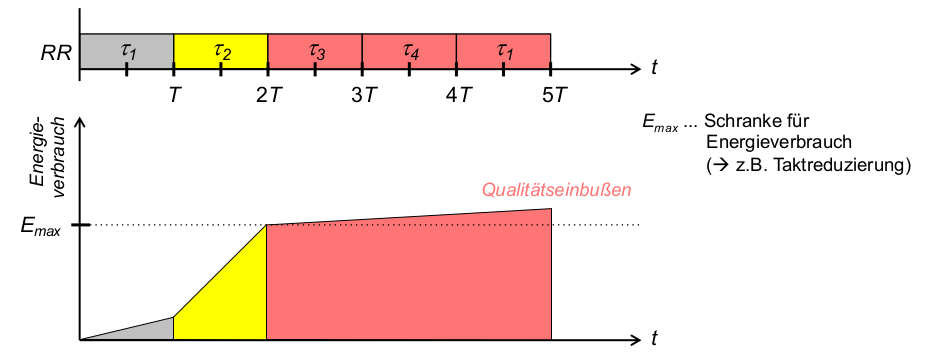
\includegraphics[width=\linewidth]{Assets/AdvancedOperatingSystems-round-robin-unfair.png} \end{itemize*}
        \item Problem 3: energieintensive Threads niedrigerer Priorität behindern spätere Threads höherer Priorität
        %\begin{itemize*}
        %\item \includegraphics[width=\linewidth]{Assets/AdvancedOperatingSystems-prioritätsumkehr.png}
        %\end{itemize*}
        \item RR Strategie 1: faire Energieverteilung (einheitliche Energielimits)
        \begin{itemize*}
            %\item 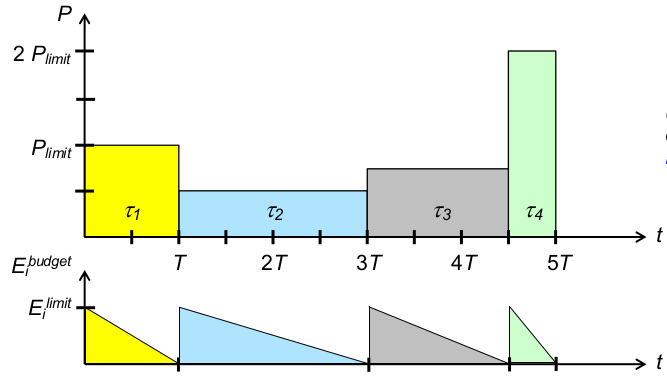
\includegraphics[width=\linewidth]{Assets/AdvancedOperatingSystems-energiebewusstes-rr.png}
            \item $1\leq i\leq 4: E_i^{limit} = P_{limit}* T$
            %\item (Abweichungen = Wichtung der Prozesse $\rightarrow$ bedingte Fairness)
        \end{itemize*}
        \item faire bzw. gewichtete Aufteilung begrenzter Energie optimiert Energieeffizienz
        \item Problem: lange, wenig energieintensive Threads verzögern Antwort-und Wartezeiten kurzer, energieintensiver Threads
        \begin{itemize*}
            \item Lösung im Einzelfall: Wichtung per $E_i^{limit}$
            \item globale Reaktivität $\rightarrow$ Nutzererfahrung?
        \end{itemize*}
        \item RR Strategie 2: maximale Reaktivität ( $\rightarrow$ klassisches RR)
        %\begin{itemize*}
        %\item \includegraphics[width=\linewidth]{Assets/AdvancedOperatingSystems-energiebewusstes-rr-reaktivität.png}
        %\end{itemize*}
        \item Problem: sparsame Threads werden bestraft durch Verfallen des ungenutzten Energiebudgets
        \item Idee: Ansparen von Energiebudgets $\rightarrow$ mehrfache Ausführung eines Threads innerhalb einer Scheduling-Periode
        \item RR Strategie 3: Reaktivität, dann faire Energieverteilung
        %\begin{itemize*}
        %\item 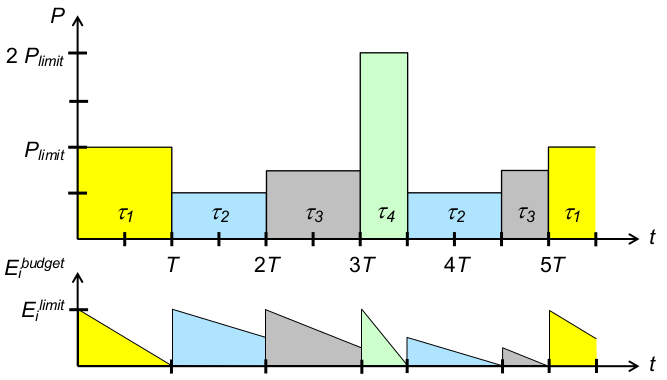
\includegraphics[width=\linewidth]{Assets/AdvancedOperatingSystems-energiebewisstes-rr-2.png}
        %\end{itemize*}
    \end{itemize*}
    Implementierungsfragen
    \begin{itemize*}
        \item Kosten ggü. klassischem RR? (durch Prioritäten...?)
        \item Scheduling-Zeitpunkte?
        \begin{itemize*}
            \item welche Accounting-Operationen (Buchführung)?
            \item wann Accounting-Operationen?
            \item wann Verdrängung?
        \end{itemize*}
        \item Datenstrukturen?
        \begin{itemize*}
            \item ... im Scheduler $\rightarrow$ Warteschlange(n)?
            \item ... im Prozessdeskriptor?
        \end{itemize*}
        \item Pro
        \begin{itemize*}
            \item Optimierung der Energieverteilung nach Schedulingzielen
            \item Berücksichtigung prozessspezifischer Verbrauchsmuster
        \end{itemize*}
        \item Kontra
        \begin{itemize*}
            \item sekundäre Kosten: Energiebedarf des Schedulers, Kontextwechsel, Implementierungskosten
            \item Voraussetzung: Monitoring des Energieverbrauchs
        \end{itemize*}
        \item \textbf{Alternative:} energieintensive Prozesse verlangsamen $\rightarrow$ Regelung der CPU-Leistungsparameter
    \end{itemize*}

    \subsubsection{Systemglobale Energieeinsparungsmaßnahmen}
    \begin{itemize*}
        \item Traditionelle: zu jedem Zeitpunkt Spitzen-Performanz angestrebt
        \begin{itemize*}
            \item viele Anwendungen benötigen keine Spitzen-Performanz
            \item viel Hardware-Zeit in Leerlaufsituationen bzw. keine Spitzen-Performanz erforderlich
        \end{itemize*}
        \item Konsequenz (besonders für mobile Systeme)
        \begin{itemize*}
            \item Hardware mit Niedrigenergiezuständen
            \item Betriebssystem kann \textbf{Energie-Management} realisieren
        \end{itemize*}
    \end{itemize*}

    \subsubsection{Hardwaretechnologien}
    DPM: Dynamic Power Management
    \begin{itemize*}
        \item versetzt leerlaufende Hardware selektiv in Zustände mit niedrigem Energieverbrauch
        \item Zustandsübergänge durch Power-Manager gesteuert, bestimmte \emph{DPM-}Strategie (Firmware) zugrunde, um gutes Verhältnis zwischen Performanz/Reaktivität und Energieeinsparung zu erzielen
        \item bestimmt, wann und wie lange eine Hardware in Energiesparmodus
    \end{itemize*}
    \begin{description*}
        \item[Greedy] Hardware-Komponente sofort nach Erreichen des Leerlaufs in Energiesparmodus, ,,Aufwecken'' durch neue Anforderung
        \item[Time-out] Energiesparmodus erst nachdem ein definiertes Intervall im Leerlauf, ,,Aufwecken'' wie bei Greedy-Strategien
        \item[Vorhersage] Energiesparmodus sofort nach Erreichen des Leerlaufs, wenn Heuristik vorhersagt,dass Kosten gerechtfertigt
        \item[Stochastisch] Energiesparmodus auf Grundlage stochastischen Modells
    \end{description*}

    DVS: Dynamic Voltage Scaling
    \begin{itemize*}
        \item effizientes Verfahren zur dynamischen Regulierung von Taktfrequenz gemeinsam mit Versorgungsspannung
        \item Nutzung quadratischer Abhängigkeit der dynamischen Leistung von Versorgungsspannung
        \item Steuerung/Strategien: Softwareunterstützung notwendig
        \item Ziel: Unterstützung von DPM-Strategien durch Maßnahmen auf Ebene von Compiler, Betriebssystem und Applikationen
        \item \textbf{Betriebssystem} (prädiktives Energiemanagement)
        \begin{itemize*}
            \item kann Benutzung verschiedener Ressourcen beobachten
            \item kann darüber Vorhersagen tätigen
            \item kann notwendigen Performanzbereich bestimmen
        \end{itemize*}
        \item \textbf{Anwendungen} können Informationen über jeweils für sie notwendige Performanz liefern
        \item[$\rightarrow$] Kombination mit energieefizientem Scheduling
    \end{itemize*}

    \subsection{Speichereffizienz}
    \begin{itemize*}
        \item  ... heißt: Auslastung des verfügbaren Speichers
        \item oft implizit: Hauptspeicherauslastung (memoryfootprint)
        \item für kleine/mobile Systeme: Hintergrundspeicherauslastung
        \item Maße zur Konkretisierung:
        \begin{itemize*}
            \item zeitlich: Maximum vs. Summe genutzten Speichers?
            \item physischer Speicherverwaltung? $\rightarrow$ Belegungsanteil pAR
            \item virtuelle Speicherverwaltung? $\rightarrow$ Belegungsanteil vAR
        \end{itemize*}
        \item Konsequenzen für Ressourcenverwaltung durch BS
        \begin{itemize*}
            \item Taskverwaltung (Accounting, Multiplexing, Fairness, ...)
            \item Programmiermodell, API (dynamische Speicherreservierung)
            \item Sinnfrage und Strategien virtueller Speicherverwaltung (VMM)
        \end{itemize*}
        \item Konsequenzen für Betriebssystem selbst
        \begin{itemize*}
            \item minimaler Speicherbedarf durch Kernel
            \item minimale Speicherverwaltungskosten (obiger Aufgaben)
        \end{itemize*}
    \end{itemize*}


    \subsubsection{Hauptspeicherauslastung}
    %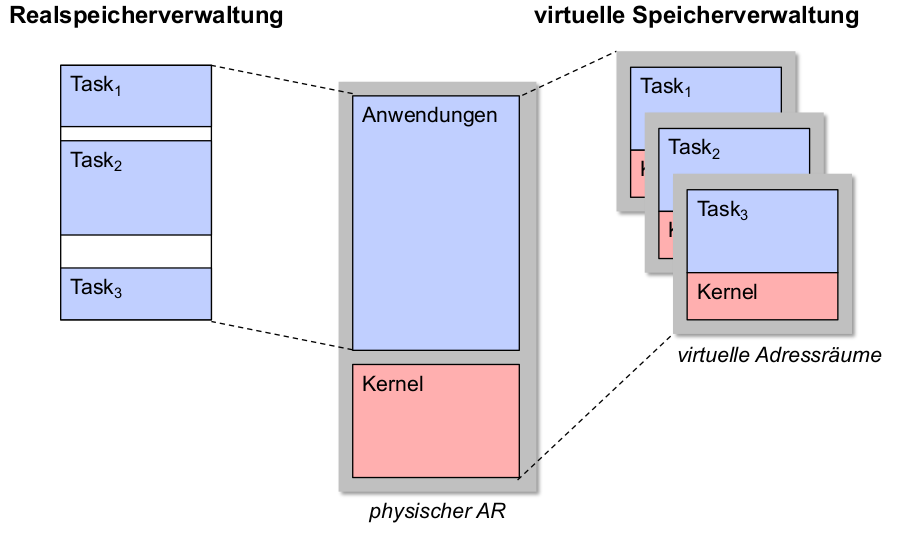
\includegraphics[width=\linewidth]{Assets/AdvancedOperatingSystems-speicherverwaltung.png}
    Problem: externe Fragmentierung
    \begin{itemize*}
        %\item 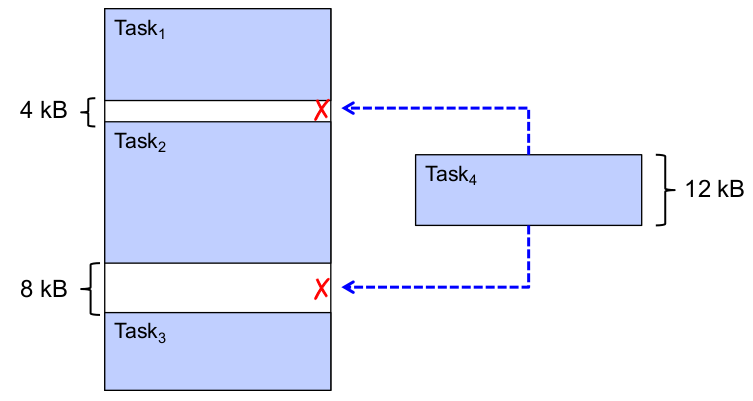
\includegraphics[width=\linewidth]{Assets/AdvancedOperatingSystems-externe-fragmentierung.png}
        \item Lösungen
        \begin{itemize*}
            \item First Fit, Best Fit, WorstFit, Buddy
            \item Relokation
        \end{itemize*}
        \item Kompromissloser Weg: kein Multitasking
    \end{itemize*}

    Problem: interne Fragmentierung
    \begin{itemize*}
        %\item 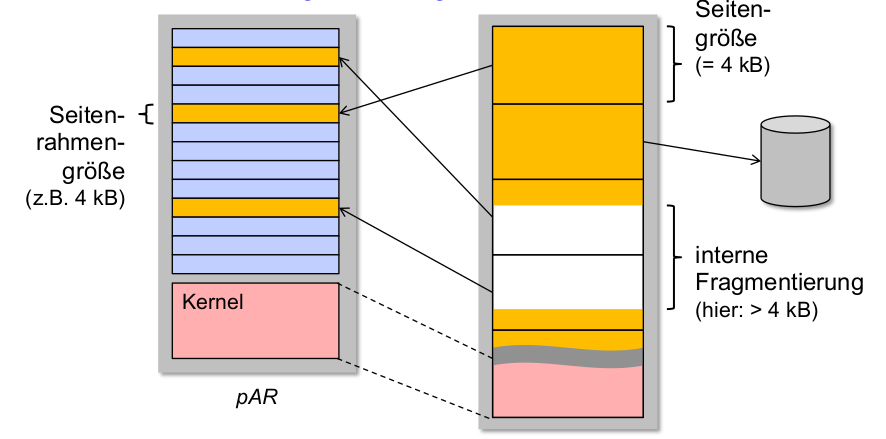
\includegraphics[width=\linewidth]{Assets/AdvancedOperatingSystems-interne-fragmentierung.png}
        \item Lösung
        \begin{itemize*}
            \item Seitenrahmengröße verringern
            \item Tradeoff: dichter belegte vAR $\rightarrow$ größere Datenstrukturen für Seitentabellen
        \end{itemize*}
        \item direkter Einfluss des Betriebssystems auf Hauptspeicherbelegung
        \begin{itemize*}
            \item[$\rightarrow$] Speicherbedarf des Kernels
            \item statische (min) Größe des Kernels (Anweisungen+Daten)
            \item dynamische Speicherreservierung durch Kernel
            \item bei Makrokernel: Speicherbedarf von Gerätecontrollern
        \end{itemize*}
    \end{itemize*}

    weitere Einflussfaktoren: Speicherverwaltungskosten
    \begin{itemize*}
        \item VMM: Seitentabellengröße $\rightarrow$ Mehrstufigkeit
        \item Metainformationen über laufende Programme: Größe von Taskkontrollblöcken (Prozess-/Threaddeskriptoren ...)
        \item dynamische Speicherreservierung durch Tasks
    \end{itemize*}

    \subsubsection{Hintergrundspeicherauslastung}
    Einflussfaktoren des Betriebssystems
    \begin{itemize*}
        \item statische Größe des Kernel-Images, beim Bootstrapping gelesen
        \item statische Größe von Programm-Images (Standards wie ELF)
        \item statisches vs. dynamisches Einbinden von Bibliotheken
        \item VMM: Größe des Auslagerungsbereichs (inkl. Teilen der Seitentabelle) für Anwendungen
        \item Modularisierung (zur Kompilierzeit) des Kernels: gezielte Anpassung an Einsatzdomäne möglich
        \item Adaptivität (zur Kompilier-und Laufzeit) des Kernels: gezielte Anpassung an sich ändernde Umgebungsbedingungen möglich
    \end{itemize*}

    \subsection{Architekturentscheidungen}
    \begin{itemize*}
        \item typische Einsatzgebiete sparsamer BS: eingebettete Systeme
        \item eingebettetes System
        \begin{itemize*}
            \item Computersystem, das in ein größeres technisches System, welches nicht zur Datenverarbeitung dient, physisch eingebunden ist
            \item Wesentlicher Bestandteil dieses größeren Systems
            \item Liefert Ausgaben in Form von Informationen/Daten
        \end{itemize*}
        \item spezielle, anwendungsspezifische Ausprägung der Aufgaben
        \begin{itemize*}
            \item reduzierter Umfang von HW-Abstraktion, hardwarenähere Ablaufumgebung
            \item begrenzte Notwendigkeit von HW-Multiplexing \& Schutz
        \end{itemize*}
        \item eng verwandte NFE: Adaptivität von sparsamen BS
        \item sparsame Betriebssysteme:
        \begin{itemize*}
            \item energieeffizient: geringe Architekturanforderungen an energieintensive Hardware
            \item speichereffizient: Auskommen mit kleinen Datenstrukturen
        \end{itemize*}
        \item Konsequenz: geringe logische Komplexität des Betriebssystemkerns
        \item sekundär: Adaptivität des Betriebssystemkerns
    \end{itemize*}

    \subsubsection{Makrokernel (monolithischer Kernel)}
    %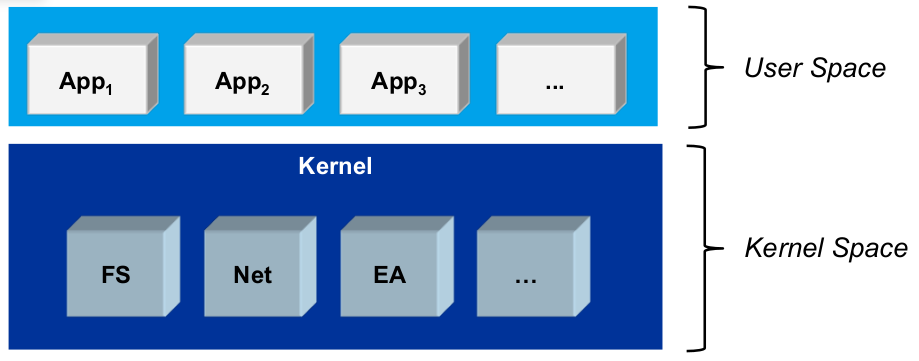
\includegraphics[width=\linewidth]{Assets/AdvancedOperatingSystems-makrokernel.png}
    \begin{itemize*}
        \item User Space:
        \begin{itemize*}
            \item Anwendungstasks
            \item CPU im unprivilegierten Modus (Unix ,,Ringe'' 1...3)
            \item Isolation von Tasks durch Programmiermodell/VMM
        \end{itemize*}
        \item Kernel Space:
        \begin{itemize*}
            \item Kernel und Gerätecontroller (Treiber)
            \item CPU im privilegierten Modus (Unix ,,Ring'' 0)
            \item keine Isolation
        \end{itemize*}
        \item Vergleich
        \begin{itemize*}
            \item[\cmark] vglw. geringe Kosten von Kernelcode (Energie, Speicher)
            \item[\cmark] VMM nicht zwingend erforderlich
            \item[\cmark] Multitasking nicht zwingend erforderlich
            \item[\xmark] Kernel (inkl. Treibern) jederzeit im Speicher
            \item[\xmark] Robustheit, Sicherheit, Adaptivität
        \end{itemize*}
    \end{itemize*}

    \subsubsection{Mikrokernel}
    %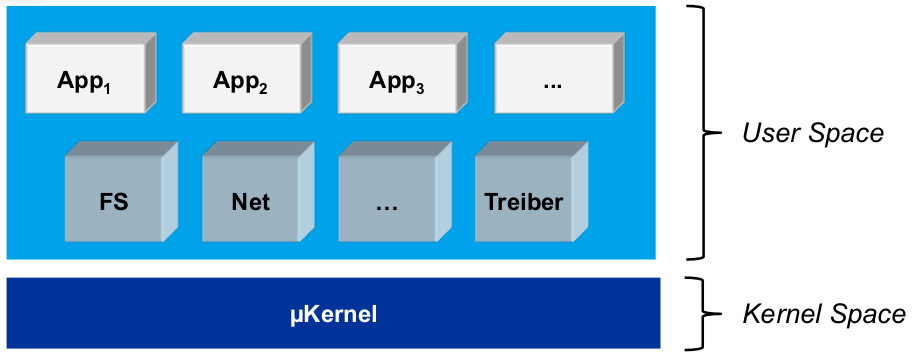
\includegraphics[width=\linewidth]{Assets/AdvancedOperatingSystems-mikrokernel.png}
    \begin{itemize*}
        \item User Space:
        \begin{itemize*}
            \item Anwendungstasks, Kernel- und Treibertasks
            \item CPU im unprivilegierten Modus
            \item Isolation von Tasks durch VMM
        \end{itemize*}
        \item Kernel Space:
        \begin{itemize*}
            \item funktional minimaler Kernel ($\mu$Kernel)
            \item CPU im privilegierten Modus
            \item keine Isolation (Kernel wird in alle vAR eingeblendet)
        \end{itemize*}
        \item Vergleich
        \begin{itemize*}
            \item[\cmark] Robustheit, Sicherheit, Adaptivität
            \item[\cmark] Kernelspeicherbedarf gering, Serverprozesse nur wenn benötigt ( $\rightarrow$ Adaptivität)
            \item[\xmark] hohe IPC-Kosten von Serverprozessen
            \item[\xmark] Kontextwechselkosten von Serverprozessen
            \item[\xmark] VMM, Multitasking i.d.R. erforderlich
        \end{itemize*}
    \end{itemize*}

    \subsubsection{BS: TinyOS}
    \begin{itemize*}
        \item Beispiel für sparsame BS im Bereich eingebetteter Systeme
        \item verbreitete Anwendung: verteilte Sensornetze (WSN)
        \item ,,TinyOS'' ist ein quelloffenes, BSD-lizenziertes Betriebssystem
        \item für drahtlose Geräte mit geringem Stromverbrauch
        \item Architektur
        \begin{itemize*}
            \item monolithisch (Makrokernel) mit Besonderheiten:
            \item keine klare Trennung zwischen der Implementierung von Anwendungen und BS (aber von funktionalen Aufgaben)
            \item[$\rightarrow$] zur Laufzeit: 1 Anwendung + Kernel
        \end{itemize*}
        \item Mechanismen:
        \begin{itemize*}
            \item kein Multithreading, keine echte Parallelität
            \item[$\rightarrow$] keine Synchronisation zwischen Tasks
            \item[$\rightarrow$] keine Kontextwechsel bei Taskwechsel
            \item Multitasking realisiert durch Programmiermodell
            \item nicht-präemptives FIFO-Scheduling
            \item kein Paging $\rightarrow$ keine Seitentabellen, keine MMU
        \end{itemize*}
        \item in Zahlen:
        \begin{itemize*}
            \item Kernelgröße: 400 Byte
            \item Kernelimagegröße: 1-4 kByte
            \item Anwendungsgröße: typisch ca. 15 kB, DB: 64 kB
        \end{itemize*}
        \item Programmiermodell:
        \begin{itemize*}
            \item BS+Anwendung als Ganzes übersetzt: statische Optimierungen durch Compiler (Laufzeit, Speicherbedarf)
            \item Nebenläufigkeit durch ereignisbasierte Kommunikation zw. Anwendung und Kernel
            \begin{itemize*}
                \item command: API-Aufruf, z.B. EA-Operation
                \item event: Reaktion auf diesen durch Anwendung
            \end{itemize*}
            \item sowohl commands als auch events : asynchron
        \end{itemize*}
    \end{itemize*}

    \subsubsection{BS: RIOT}
    \begin{itemize*}
        \item sparsames BS,optimiert für anspruchsvollere Anwendungen
        \item Open-Source-Mikrokernel-basiertes Betriebssystem für IoT
        \item Architektur
        \begin{itemize*}
            \item halbwegs: Mikrokernel
            \item energiesparende Kernelfunktionalität
            \begin{itemize*}
                \item minimale Algorithmenkomplexität
                \item vereinfachtes Threadkonzept $\rightarrow$ keine Kontextsicherung erforderlich
                \item keine dynamische Speicherallokation
                \item energiesparende Hardwarezustände vom Scheduler ausgelöst (inaktive CPU)
            \end{itemize*}
            \item Mikrokerneldesign unterstützt komplementäre NFE: Adaptivität, Erweiterbarkeit
            \item Kosten: IPC (hier gering)
        \end{itemize*}
        \item Mechanismen:
        \begin{itemize*}
            \item Multithreading-Programmiermodell
            \item modulare Implementierung von Dateisystemen, Scheduler, Netzwerkstack
        \end{itemize*}
        \item in Zahlen:
        \begin{itemize*}
            \item Kernelgröße: 1,5 kByte
            \item Kernelimagegröße: 5 kByte
        \end{itemize*}
    \end{itemize*}

    \section{Robustheit und Verfügbarkeit}
    Motivation
    \begin{itemize*}
        \item allgemein: verlässlichkeitskritische Anwendungsszenarien
        \item Forschung in garstiger Umwelt (Weltraum)
        \item hochsicherheitskritische Systeme (Finanz, Cloud Dienste)
        \item hochverfügbare System (öffentliche Infrastruktur, Strom)
        \item HPC (high performance computing)
    \end{itemize*}

    Allgemeine Begriffe
    \begin{itemize*}
        \item Verlässlichkeit: Fähigkeit, eine Leistung zu erbringen, der man berechtigterweise vertrauen kann
        \item Untereigenschaften
        \begin{enumerate*}
            \item Verfügbarkeit (availability)
            \item Robustheit (robustness, reliability
            \item (Funktions-) Sicherheit (safety)
            \item Vertraulichkeit (confidentiality)
            \item Integrität (integrity)
            \item Wartbarkeit (maintainability) (vgl.: evolutionäre Eigenschaften)
        \end{enumerate*}
        \item[$\rightarrow$] nicht für alle Anwendungen sind alle Untereigenschaften erforderlich
    \end{itemize*}

    \subsubsection{Robustheitsbegriff}
    \begin{itemize*}
        \item Untereigenschaften von Verlässlichkeit: Robustheit (reliability)
        \item Ausfall: beobachtbare Verminderung der Leistung eines Systems, gegenüber seiner als korrekt spezifizierten Leistung
        \item Robustheit: Verlässlichkeit unter Anwesenheit externer Ausfälle (= Ursache außerhalb des betrachteten Systems)
    \end{itemize*}

    \subsubsection{Fehler, Ausfälle und ihre Vermeidung}
    \begin{itemize*}
        \item Fehler $\rightarrow$ fehlerhafter Zustand $\rightarrow$ Ausfall
        %\item 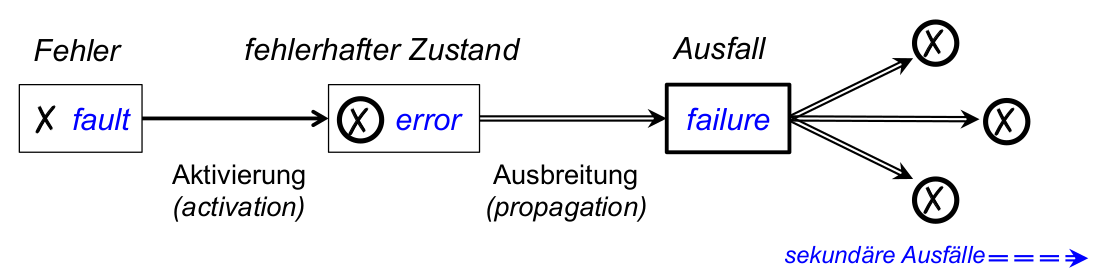
\includegraphics[width=\linewidth]{Assets/AdvancedOperatingSystems-fehler.png}
    \end{itemize*}
    \begin{description*}
        \item[Ausfall] (failure) liegt vor, wenn tatsächliche Leistung(en), die ein System erbringt, von als korrekt spezifizierter Leistung abweichen
        \begin{itemize*}
            \item Korrektheit testen/beweisen( $\rightarrow$ formale Verifikation)
        \end{itemize*}
        \item[fehlerhafter Zustand] (error) notwendige Ursache eines Ausfalls (nicht jeder error muss zu failure führen)
        \begin{itemize*}
            \item Maskierung, Redundanz
            \item Isolation von Subsystemen
            \item[$\rightarrow$] Isolationsmechanismen
        \end{itemize*}
        \item[Fehler] (fault) Ursache für fehlerhaften Systemzustand ( error ), z.B. Programmierfehler
        \begin{itemize*}
            \item Ausfallverhalten spezifizieren
            \item Ausfälle zur Laufzeit erkennen und Folgen beheben, abschwächen...
            \item[$\rightarrow$] Micro-Reboots
        \end{itemize*}
    \end{description*}

    \subsection{Fehlerhafter Zustand}
    interner und externer Zustand (internal \& external state)
    \begin{itemize*}
        \item externer Zustand: der Teil des Gesamtzustands, der an externer Schnittstelle sichtbar wird
        \item interner Zustand: restlicher Teilzustand
        \item erbrachte Leistung: zeitliche Folge externer Zustände
    \end{itemize*}
    Fehlerausbreitung und (externer) Ausfall
    \begin{itemize*}
        \item Wirkungskette: Treiber-Programmierfehler (fault) $\rightarrow$ fehlerhafter interner Zustand des Treibers (error)
        \begin{itemize*}
            \item Ausbreitung dieses Fehlers (failure des Treibers)
            \item[$\Rightarrow$] fehlerhafter externer Zustand des Treibers
            \item[$\Rightarrow$] fehlerhafter interner Zustand des Kernels (error)
            \item[$\Rightarrow$] Kernelausfall (failure)
        \end{itemize*}
        \item Auswirkung: fehlerhafter Zustand weiterer Kernel-Subsysteme
        \item[$\rightarrow$] Robustheit: Isolationsmechanismen
        %\item 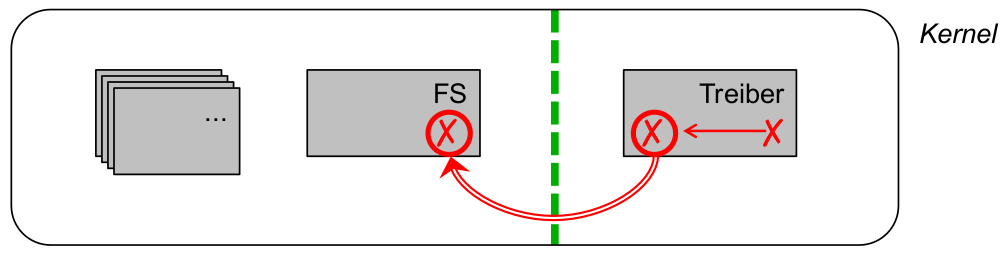
\includegraphics[width=\linewidth]{Assets/AdvancedOperatingSystems-treiber-kernel-fehler.png}
    \end{itemize*}

    \subsection{Isolationsmechanismen}
    \begin{itemize*}
        \item Isolationsmechanismen für robuste Betriebssysteme
        \begin{itemize*}
            \item durch strukturierte Programmierung
            \item durch Adressraumisolation
        \end{itemize*}
        \item noch mehr für sichere Betriebssysteme
        \begin{itemize*}
            \item durch kryptografische Hardwareunterstützung: Enclaves
            \item durch streng typisierte Sprachen und managed code
            \item durch isolierte Laufzeitumgebungen: Virtualisierung
        \end{itemize*}
    \end{itemize*}

    \subsubsection{Strukturierte Programmierung}
    Monolithisches BS... in historischer Reinform:
    \begin{itemize*}
        \item Anwendungen, Kernel, gesamte BS-Funktionalität
        \item programmiert als Sammlung von Prozeduren
        \item jede darf jede davon aufrufen, keine Modularisierung
        \item keine definierten internen Schnittstellen
    \end{itemize*}

    Monolithisches Prinzip
    \begin{itemize*}
        \item Ziel: Isolation zwischen Anwendungen und Betriebssystem
        \item Mechanismus: Prozessor-Privilegierungsebenen (user/kernelspace)
        \item Konsequenz: fast keine Strukturierung des Kernels
        %\item \includegraphics[width=\linewidth]{Assets/AdvancedOperatingSystems-systemaufruf.png}
    \end{itemize*}

    Strukturierte Makrokernarchitektur
    \begin{itemize*}
        \item schwach strukturierter (monolithischer) Makrokernel
        %\item 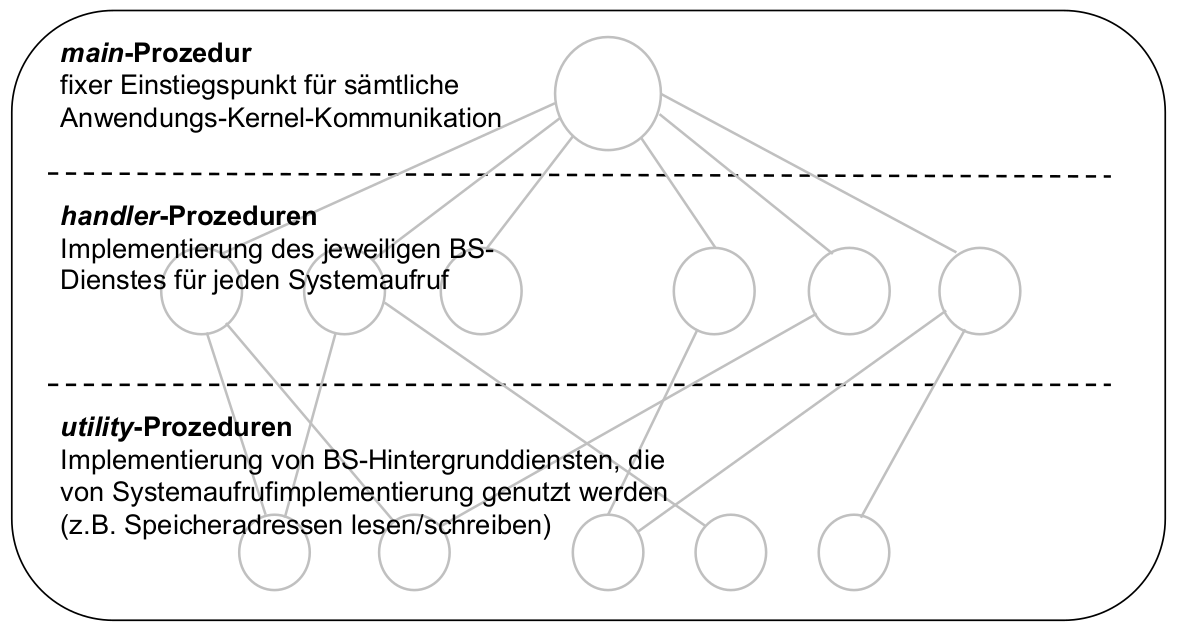
\includegraphics[width=\linewidth]{Assets/AdvancedOperatingSystems-makrokernelarchitektur.png}
        \item[$\Rightarrow$] Schichtendifferenzierung ( layered operating system )
        \item Modularisierung
    \end{itemize*}
    Modularer Makrokernel
    \begin{itemize*}
        \item Kernelfunktionen in Module unterteilt $\rightarrow$ Erweiter-/Portierbarkeit
        \item klar definierte Modulschnittstellen
        \item Module zur Kernellaufzeit dynamisch einbindbar (Adaptivität)
    \end{itemize*}

    \paragraph{Fehlerausbreitung beim Makrokernel}
    \begin{itemize*}
        \item[\cmark] Wartbarkeit
        \item[\cmark] Portierbarkeit
        \item[\cmark] Erweiterbarkeit
        \item (begrenzt) Adaptivität
        \item Schutz gegen statische Programmierfehler nur durch Compiler
        \item[\xmark] kein Schutz gegen dynamische Fehler
    \end{itemize*}

    \subsubsection{Adressraumisolation}
    Private virtuelle Adressräume und Fehlerausbreitung
    \begin{itemize*}
        \item private virtuelle Adressräume zweier Tasks ($i\not= j$)
        %\item private virtuelle vs. physischer Adresse
        %\begin{itemize*}
        %\item 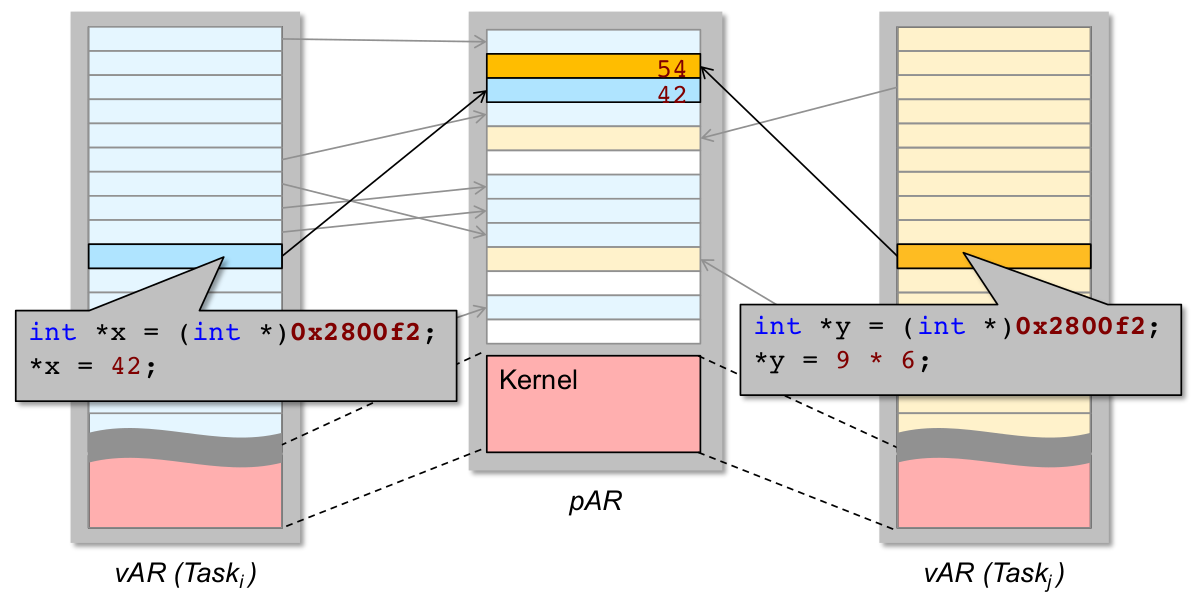
\includegraphics[width=\linewidth]{Assets/AdvancedOperatingSystems-virtuelle-vs-physische-adresse.png}
        %\end{itemize*}
        \item korrekte private vAR: kollisionsfreie Seitenabbildung
        \item Magie in Hardware: MMU (BS steuert und verwaltet...)
    \end{itemize*}
    Robustheit: Vorteil von privaten vAR?
    \begin{itemize*}
        \item[\cmark] nichtvertrauenswürdiger Code kann keine beliebigen physischen Adressen schreiben
        \item[\cmark] Kommunikation zwischen nvw. Code muss durch IPC-Mechanismen explizit hergestellt werden $\rightarrow$ Überwachung und Validierung zur Laufzeit möglich
        \item[\cmark] Kontrollfluss begrenzen: Funktionsaufrufe können i.A. keine AR-Grenzen überschreiten
        \begin{itemize*}
            \item[$\rightarrow$] BS-Zugriffssteuerung kann nicht durch Taskfehler ausgehebelt werden
            \item[$\rightarrow$] unabsichtliche Terminierungsfehler(unendliche Rekursion) erschwert ...
        \end{itemize*}
        \item keine Isolation zwischen Fehlern innerhalb des Kernels
    \end{itemize*}

    \subsection{Mikrokernelarchitektur}
    Fortschritt ggü. Makrokernel
    \begin{itemize*}
        \item Strukturierungskonzept
        \begin{itemize*}
            \item strenger durchgesetzt durch konsequente Isolation voneinander unabhängiger Kernel-Subsysteme
            \item zur Laufzeit durchgesetzt $\rightarrow$ Reaktion auf fehlerhafte Zustände möglich!
        \end{itemize*}
        \item zusätzlich zu vertikaler Strukturierung des Kernels: horizontale Strukturierung eingeführt
        \begin{itemize*}
            \item[$\rightarrow$] funktionale Einheiten: vertikal (Schichten)
            \item[$\rightarrow$] isolierte Einheiten: horizontal (private vAR)
        \end{itemize*}
        \item[$\Rightarrow$] Kernel (alle BS-Funktionalität) $\rightarrow$ $\mu$Kernel (minimale BS-Funk.)
        \item Rest: ,,gewöhnliche'' Anwendungsprozesse mit AR-isolation
        \item Kommunikation: botschaftenbasierte IPC (client-server OS)
        \item Nomenklatur: Mikrokernel und Serverprozesse
    \end{itemize*}

    \subsubsection{Modularer Makrokernel vs. Mikrokernel}
    \begin{itemize*}
        %\item 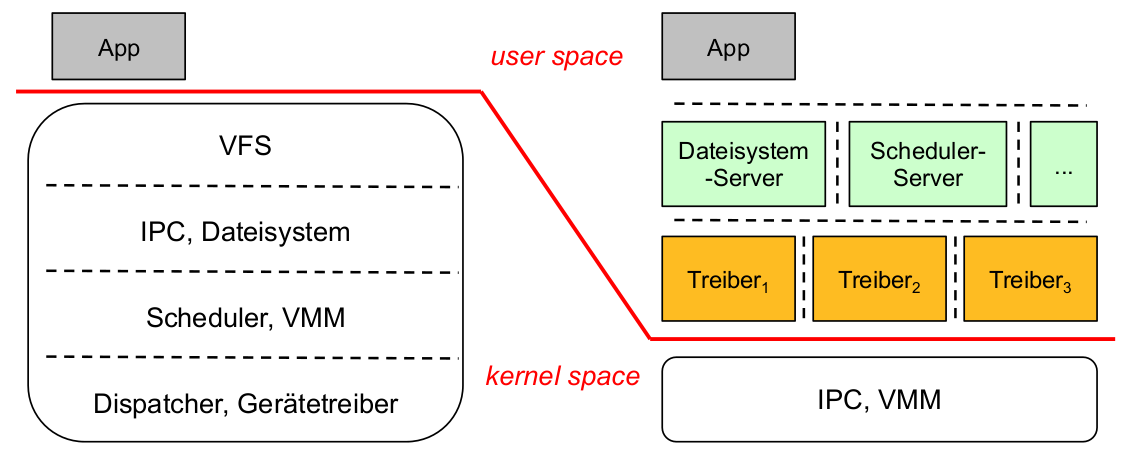
\includegraphics[width=\linewidth]{Assets/AdvancedOperatingSystems-modularer-makrokernel.png}
        \item minimale Kernelfunktionalität:
        \item keine Dienste, nur allgemeine Schnittstellenfür diese
        \item keine Strategien, nur grundlegende Mechanismen zur Ressourcenverwaltung
        \item neues Problem: minimales Mikrokerneldesign
        %\item 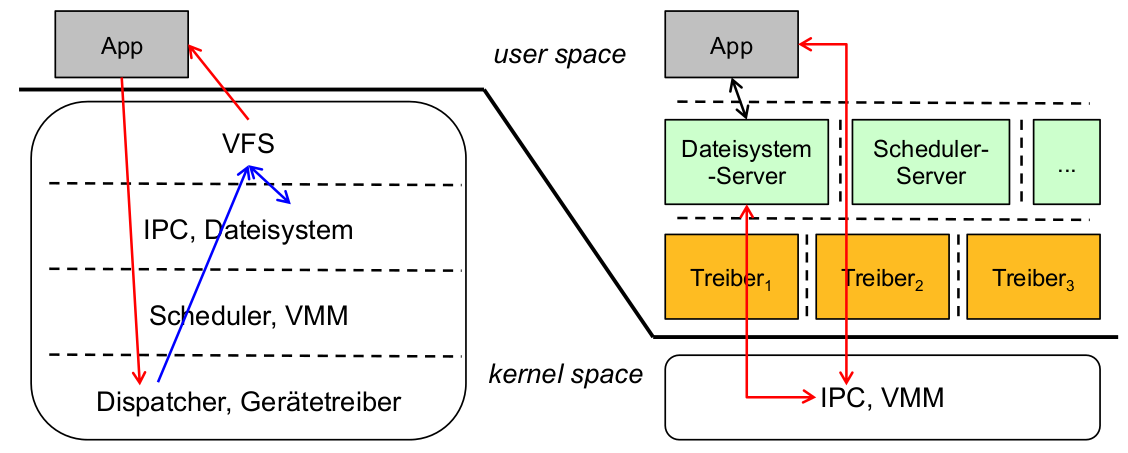
\includegraphics[width=\linewidth]{Assets/AdvancedOperatingSystems-modularer-makrokernel-2.png}
    \end{itemize*}

    \paragraph{Robustheit von Mikrokernen}
    \begin{itemize*}
        \item = Gewinn durch Adressraumisolation innerhalb des Kernels
        \item[\cmark] kein nichtvertrauenswürdiger Code im Kernelspace, der dort beliebige physische Adressen manipulieren kann
        \item[\cmark] Kommunikation zwischen nvw. Code (nicht zur zwischen Anwendungstasks)muss durch IPC explizit hergestellt werden $\rightarrow$ Überwachung und Validierung zur Laufzeit
        \item[\cmark] Kontrollfluss begrenzen: Zugriffssteuerung auch zwischen Serverprozessen, zur Laufzeit unabhängiges Teilmanagement von Code (Kernelcode) möglich (z.B.: Nichtterminierung erkennen)
        \item Neu:
        \item[\cmark] nvw. BS-Code muss nicht mehr im Kernelspace laufen
        \item[\cmark] verbleibender Kernel: klein, funktional weniger komplex, leichter zu entwickeln, zu testen, evtl. formal zu verifizieren
        \item[\cmark] daneben: Adaptivität durch konsequentere Modularisierung des Kernels gesteigert
    \end{itemize*}

    \subsubsection{Mikrokernel: Mach}
    \begin{itemize*}
        \item 1975: Aleph (BS des ,,Rochester Intelligent Gateway'')
        \item 1979/81: Accent (verteiltes BS), CMU
        \item Mach 3.0 (1989): einer der ersten praktisch nutzbaren $\mu$Kerne
        \item Ziel: API-Emulation ($\not=$ Virtualisierung) von UNIX und -Derivaten auf unterschiedlichen Prozessorarchitekturen
        \item mehrere unterschiedliche Emulatoren gleichzeitig lauffähig
        \begin{itemize*}
            \item Emulation außerhalb des Kernels
            \item Komponente im Adressraum des Applikationsprogramms
            \item $1...n$ Server, unabhängig von Applikationsprogramm
        \end{itemize*}
    \end{itemize*}

    $\mu$Kernel-Funktionen
    \begin{enumerate*}
        \item Prozessverwaltung
        \item Speicherverwaltung
        \item IPC-und E/A-Dienste, einschließlich Gerätetreiber
    \end{enumerate*}

    unterstützte Abstraktionen ( $\rightarrow$ API, Systemaufrufe):
    \begin{enumerate*}
        \item Prozesse, Threads, Speicherobjekte
        \item Ports (generisches, ortstransparentes Adressierungskonzept)
        \item Botschaften, ... (sekundäre, von den obigen genutzte Abstraktionen)
    \end{enumerate*}

    Architektur
    \begin{itemize*}
        %\item 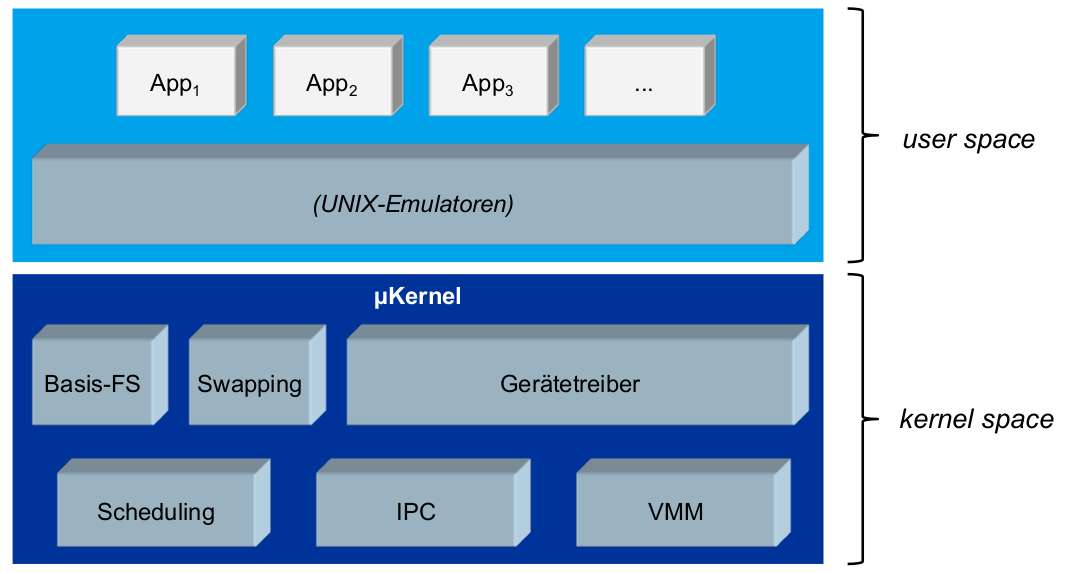
\includegraphics[width=\linewidth]{Assets/AdvancedOperatingSystems-mach-architektur.png}
        \item Systemaufrufkosten:
        \begin{itemize*}
            \item IPC-Benchmark (1995): i486 Prozessor, 50 MHz
            \item Messung mit verschiedenen Botschaftenlängen( x - Werte)
            \item ohne Nutzdaten (0 Byte Botschaftenlänge): 115 $\mu$s (Tendenz unfreundlich ...)
            %\item 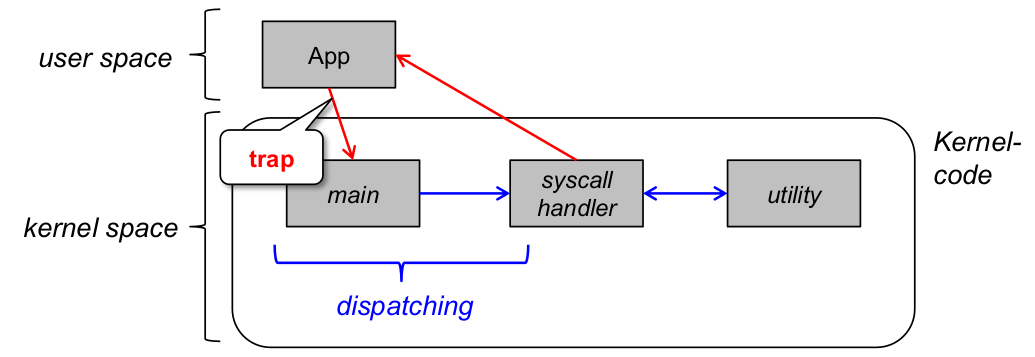
\includegraphics[width=\linewidth]{Assets/AdvancedOperatingSystems-mach-systemaufruf.png}
        \end{itemize*}
        \item Bewertung aus heutiger Sicht:
        \begin{itemize*}
            \item funktional komplex
            \item 153 Systemaufrufe
            \item mehrere Schnittstellen, parallele Implementierungen für eine Funktion
            \item[$\rightarrow$] Adaptivität (Auswahl durch Programmierer)
        \end{itemize*}
        \item Fazit:
        \begin{itemize*}
            \item zukunftsweisender Ansatz
            \item langsame und ineffiziente Implementierung
        \end{itemize*}
    \end{itemize*}

    Lessons Learned
    \begin{itemize*}
        \item Umsetzung: Designkriterien weitgehend unbekannt
        \item Folgen für Performanz und Programmierkomfort: [Heis19]
        \item[\xmark] ,,complex'', ,,inflexible'', ,,slow''
        \item wissen etwas über Kosten: IPC-Performanz, Kernelabstraktionen
        \item wissen nichts über guten $\mu$Kern-Funktionsumfang und gute Schnittstellen
    \end{itemize*}

    \subsubsection{L4}
    Analyse des Mach-Kernels:
    \begin{enumerate*}
        \item falsche Abstraktionen
        \item unperformante Kernelimplementierung
        \item prozessorunabhängige Implementierung
    \end{enumerate*}

    L3 und L4
    \begin{itemize*}
        \item Mikrokerne der 2. Generation
        \item vollständige Überarbeitung des Mikrokernkonzepts
    \end{itemize*}
    \begin{tabular}{c|c|c}
        First generation                                                                      & Second Generation    & Third generation  \\\hline
        Eg Mach                                                                               & Eg L4                & seL4              \\
        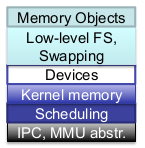
\includegraphics[width=.2\linewidth]{Assets/AdvancedOperatingSystems-l4-first-g.png}  &
        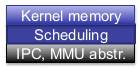
\includegraphics[width=.2\linewidth]{Assets/AdvancedOperatingSystems-L4-second-g.png} &
        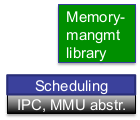
\includegraphics[width=.2\linewidth]{Assets/AdvancedOperatingSystems-l4-third-g.png}                                             \\
        180 syscalls                                                                          & $\sim$ 7 syscalls    & $\sim$ 3 syscalls \\
        100 kLOC                                                                              & $\sim$ 10 kLOC       & 9 kLOC            \\
        100 $\mu s$ IPC                                                                       & $\sim$ 1 $\mu s$ IPC & $0,2-1 \mu s$ IPC
    \end{tabular}

    \subsubsection{Mikrokernel - Designprinzipien}
    \begin{itemize*}
        \item Was gehört in einen Mikrokern?
        \item Konzeptsicht $\rightarrow$ Funktionalität
        \item Implementierungssicht $\rightarrow$ Performanz
        \item[$\rightarrow$] 1. Generation: durch Performanzentscheidungen aufgeweicht
        \item[$\rightarrow$] Effekt in Praxis gegenteilig: schlechte (IPC-) Performanz
    \end{itemize*}

    Designprinzipien für Mikrokernel-Konzept
    \begin{enumerate*}
        \item System interaktive und nicht vollständig vertrauenswürdige Applikationen unterstützen ( $\rightarrow$ HW-Schutz,-Multiplexing),
        \item Hardware mit virtueller Speicherverwaltung und Paging
    \end{enumerate*}

    Designprinzipien
    \begin{description*}
        \item[Autonomie] Subsystem muss so implementiert werden, dass es von keinem anderen Subsystem gestört oder korrumpiert werden kann
        \item[Integrität] Subsystem $S_1$ muss sich auf Garantien von $S_2$ verlassen können. D.h. beide Subsysteme müssen miteinander kommunizieren können, ohne dass ein drittes Subsystem diese Kommunikation stören, fälschen oder abhören kann.
    \end{description*}

    L4: Speicherabstraktion
    \begin{itemize*}
        \item Adressraum: Abbildung, die jede virtuelle Seite auf einen physischen Seitenrahmen abbildet oder als ,,nicht zugreifbar'' markiert
        \item Implementierung über Seitentabellen, unterstützt durch MMU-Hardware
        \item Aufgabe des Mikrokernels (Schicht aller Subsysteme): muss Hardware-Konzept des Adressraums verbergen und durch eigenes Adressraum-Konzept überlagern
        \item Mikrokernel-Konzept des Adressraums:
        \begin{itemize*}
            \item muss Implementierung von beliebigen virtuellen Speicherverwaltungs-und -schutzkonzepten oberhalb des Mikrokernels (d.h. in den Subsystemen) erlauben
            \item sollte einfach und dem Hardware-Konzept ähnlich sein
        \end{itemize*}
        \item Idee: abstrakte Speicherverwaltung
        \begin{itemize*}
            \item rekursive Konstruktion und Verwaltung der Adressräume auf Benutzer-(Server-)Ebene
            \item Mikrokernel stellt dafür genau drei Operationen bereit:
        \end{itemize*}
    \end{itemize*}
    \begin{description*}
        \item[grant(x)] Server überträgt Seite $x$ seines AR in AR von Empfänger
        \item[map(x)] Server bildet Seite $x$ seines AR in AR von Empfänger ab
        \item[flush(x)] Server entfernt Seite x seines AR aus allen fremden AR
    \end{description*}

    Hierarchische Adressräume
    \begin{itemize*}
        \item Rekursive Konstruktion der Adressraumhierarchie
        \item Server und Anwendungenkönnen damit ihren Klienten Seiten des eigenen Adressraumes zur Verfügung stellen
        \item Realspeicher: Ur-Adressraum vom $\mu$Kernel verwaltet
        \item Speicherverwaltung, Paging... außerhalb des $\mu$-Kernels realisiert
        %\item 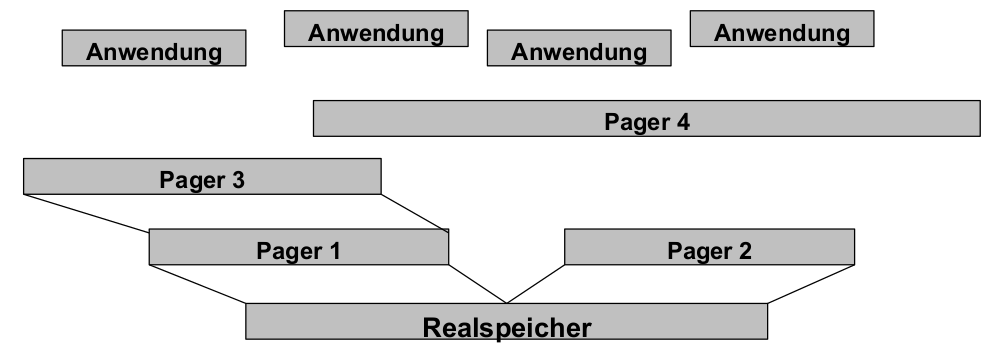
\includegraphics[width=\linewidth]{Assets/AdvancedOperatingSystems-adressraumhierarchie.png}
    \end{itemize*}

    L4: Threadabstraktion
    \begin{itemize*}
        \item Thread
        \begin{itemize*}
            \item innerhalb eines Adressraumes ablaufende Aktivität
            \item[$\rightarrow$] Adressraumzuordnung essenziell für Threadkonzept
            \item Bindung an Adressraum: dynamisch oder fest
            \item Änderung einer dynamischen Zuordnung: darf nur unter vertrauenswürdiger Kontrolle erfolgen
        \end{itemize*}
        \item Designentscheidung
        \begin{itemize*}
            \item[$\rightarrow$] Autonomieprinzip
            \item[$\rightarrow$] Konsequenz: Adressraumisolation
            \item[$\rightarrow$] entscheidender Grund zur Realisierung des Thread-Konzepts innerhalb des Mikrokernels
        \end{itemize*}
    \end{itemize*}

    IPC
    \begin{itemize*}
        \item Interprozess-Kommunikation
        \begin{itemize*}
            \item Kommunikation über Adressraumgrenzen
            \item vertrauenswürdig kontrollierte Aufhebung der Isolation
            \item[$\rightarrow$] essenziell für (sinnvolles) Multitasking und -threading
        \end{itemize*}
        \item Designentscheidung
        \begin{itemize*}
            \item[$\rightarrow$] Integritätsprinzip
            \item[$\rightarrow$] vertrauenswürdige Adressraumisolation im $\mu$Kernel
            \item[$\rightarrow$] grundlegendes IPC-Konzepts innerhalb des Mikrokernels
        \end{itemize*}
    \end{itemize*}

    Identifikatoren
    \begin{itemize*}
        \item Thread-und Ressourcenbezeichner
        \begin{itemize*}
            \item müssen vertrauenswürdig vergeben und verwaltet werden
            \item[$\rightarrow$] essenziell für (sinnvolles) Multitasking und -threading
            \item[$\rightarrow$] essenziell für vertrauenswürdige Kernel-/Server-Schnittstellen
        \end{itemize*}
        \item Designentscheidung
        \begin{itemize*}
            \item[$\rightarrow$] Integritätsprinzip
            \item[$\rightarrow$] ID-Konzept innerhalb des Mikrokernels
        \end{itemize*}
    \end{itemize*}

    Lessons Learned
    \begin{enumerate*}
        \item Ein minimaler Mikrokernel
        \begin{itemize*}
            \item stellt Minimalmenge geeigneter Abstraktionen verfügbar
            \item flexibel, um Implementierung beliebiger BS zu ermöglichen
            \item Nutzung verschiedener Hardware-Plattformen
        \end{itemize*}
        \item Geeignete, funktional minimale Mechanismen im $\mu$Kern:
        \begin{itemize*}
            \item Adressraum mit map-, flush-, grant-Operation
            \item Threadsinklusive IPC
            \item eindeutige Identifikatoren
        \end{itemize*}
        \item Wahl der geeigneten Abstraktionen: kritisch für Verifizierbarkeit, Adaptivität und optimierte Performanz des Mikrokerns
        \item Bisherigen $\mu$-Kernel-Abstraktionskonzepte: ungeeignete, zu viele, zu spezialisierte u. inflexible Abstraktionen
        \item Konsequenzen für Mikrokernel-Implementierung
        \begin{itemize*}
            \item müssen für jeden Prozessortyp neu implementiert werden
            \item deshalb prinzipiell nicht portierbar $\rightarrow$ L3-/L4-Prototypen: 99\% Assemblercode
        \end{itemize*}
        \item innerhalb eines Mikrokernels sind von Prozessorhardware abhängig
        \begin{enumerate*}
            \item grundlegende Implementierungsentscheidungen
            \item meiste Algorithmen u. Datenstrukturen
        \end{enumerate*}
        \item Fazit: Mikrokernel mit akzeptabler Performanz hardwarespezifische Implementierung minimal erforderlicher vom Prozessortyp unabhängiger Abstraktionen
        %\item 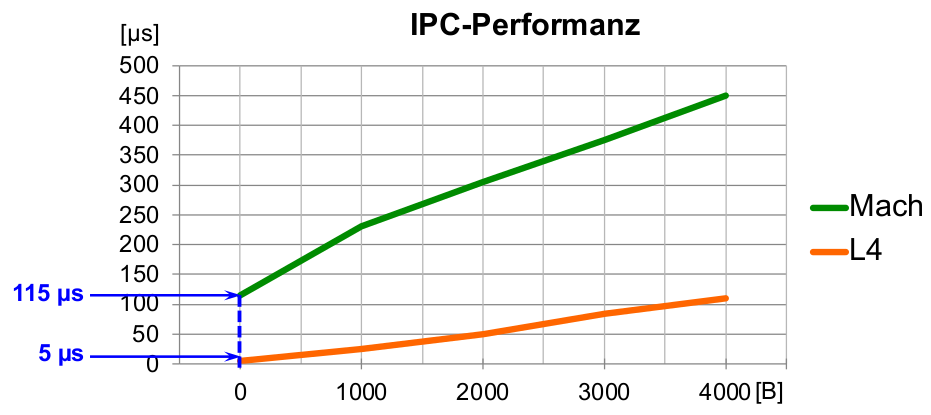
\includegraphics[width=\linewidth]{Assets/AdvancedOperatingSystems-l4-ipc-performance.png}
        \item L4 heute: Spezifikation Mikrokernels (nicht Implementierung)
    \end{enumerate*}

    %Einige Weiterentwicklungen:
    %\begin{itemize*}
    %    \item TU Dresden (Hermann Härtig): Neuimplementierung in C++ (L4/Fiasco), Basis des Echtzeit-Betriebssystems DROPS, der Virtualisierungsplattform NOVA und des adaptiven BS-Kernels Fiasco.OC
    %    \item University of New South Wales, Australien
    %    \begin{itemize*}
    %        \item Implementierung von L4 auf verschiedenen 64 - Bit-Plattformen, bekannt als L4/MIPS, L4/Alpha
    %        \item Implementierung in C (Wartbarkeit, Performanz)
    %        \item Mit L4Ka::Pistachio bisher schnellste Implementierung von botschaftenbasierterIPC
    %        \item 2009: seL4, erster formal verifizierter BS-Kernel
    %    \end{itemize*}
    %\end{itemize*}

    Zwischenfazit
    \begin{itemize*}
        \item Begrenzung von Fehlerausbreitung ($\rightarrow$ Folgen von errors)
        \item konsequent modularisierte Architektur aus Subsystemen
        \item Isolationsmechanismen zwischen Subsystemen
        \item statische Isolation auf Quellcodeebene $\rightarrow$ strukturierte Programmierung
        \item dynamische Isolation zur Laufzeit $\rightarrow$ private virtuelle Adressräume
        \item Architektur, welche diese Mechanismen komponiert: Mikrokernel
        \item[\cmark] Adressraumisolation für sämtlichen nichtvertrauenswürdigen Code
        \item[\cmark] keine privilegierten Instruktionen in nvw. Code (Serverprozesse)
        \item[\cmark] geringe Größe (potenziell: Verifizierbarkeit) des Kernels
        \item[\cmark] neben Robustheit: Modularitätund Adaptivitätdes Kernels
        \item[\xmark] Behandlung von Ausfällen ( $\rightarrow$ abstürzende Gerätetreiber ...)
    \end{itemize*}

    \subsection{Micro-Reboots}
    \begin{itemize*}
        \item Kernelfehler potentiell fatal für gesamtes System
        \item Anwendungsfehler nicht
        \item[$\rightarrow$] kleiner Kernel = geringeres Risiko von Systemausfällen
        \item[$\rightarrow$] BS-Code in Serverprozessen: verbleibendes Risiko unabhängiger Teilausfälle von BS-Funktionalität
        \item Ergänzung zu Isolationsmechanismen notwendig
        \item Mechanismen zur Behandlung von Subsystem-Ausfällen
        \item[=] Mechanismen zur Behandlung Anwendungs-, Server- und Gerätetreiberfehlen
        \item[$\rightarrow$] Micro-Reboots
    \end{itemize*}

    Ansatz
    \begin{itemize*}
        \item kleinen (als fehlerfrei angenommenen) $\mu$Kernel
        \item BS-Funktionalität in bedingt vertrauenswürdigen Serverprozessen %(kontrollierbare, aber wesentlich größere Codebasis)
        \item Treiber/Anwendungen in nicht vertrauenswürdigen Prozessen %(nicht kontrollierbare Codebasis)
        \item wollen Systemausfälle verhindern durch Vermeidung von errors im Kernel $\rightarrow$ höchste Priorität
        \item Treiber-und Serverausfälle minimieren durch Verbergen ihrer Auswirkungen $\rightarrow$ nachgeordnete Priorität (Best-Effort-Prinzip)
        \item Idee: Ausfälle $\rightarrow$ Neustart durch spezialisierten Serverprozess
    \end{itemize*}

    %Beispiel: Ethernet-Treiberausfall
    %\begin{itemize*}
    %\item 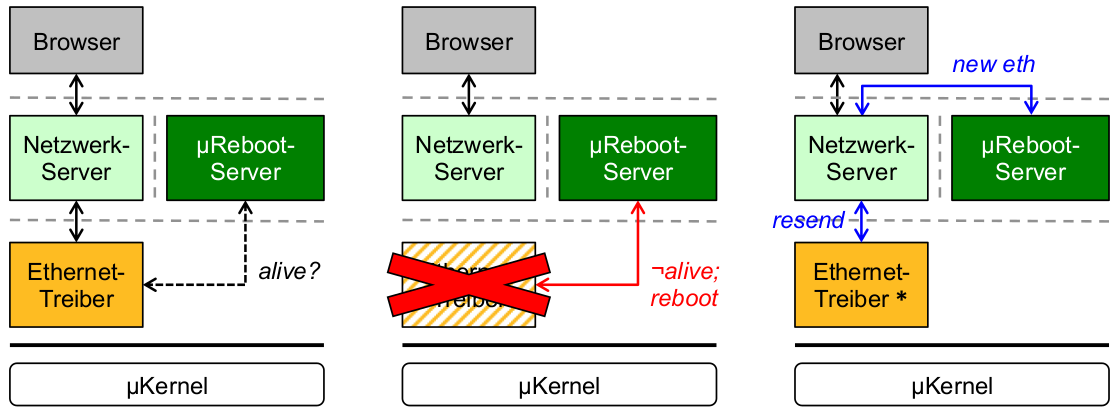
\includegraphics[width=\linewidth]{Assets/AdvancedOperatingSystems-ethernet-treiberausfall.png}
    %    \item schwarz: ausfallfreie Kommunikation
    %    \item rot: Ausfall und Behandlung
    %    \item blau: Wiederherstellung nach Ausfall
    %\end{itemize*}

    %Beispiel: Dateisystem-Serverausfall
    %\begin{itemize*}
    %    %\item 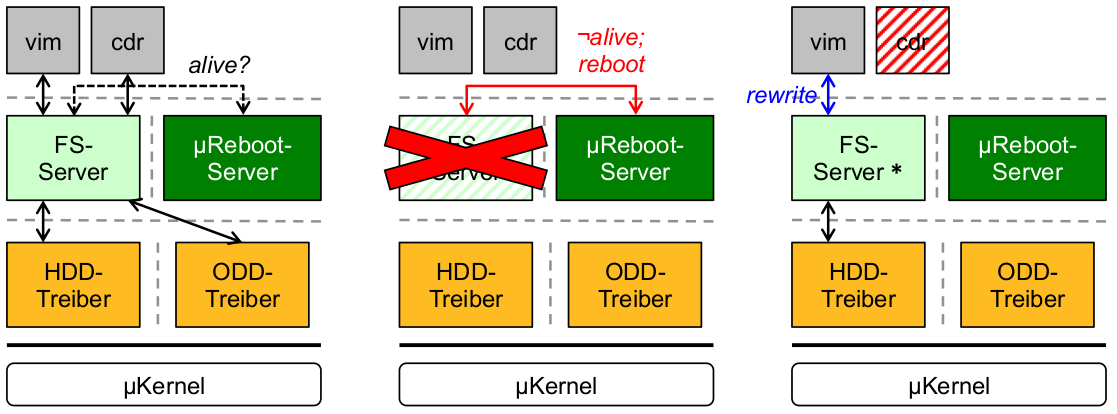
\includegraphics[width=\linewidth]{Assets/AdvancedOperatingSystems-dateisystem-serverausfall.png}
    %    \item schwarz: ausfallfreie Kommunikation
    %    \item rot: Ausfall und Behandlung
    %    \item blau: Wiederherstellung nach Ausfall
    %\end{itemize*}

    \subsubsection{Beispiel-Betriebssystem: MINIX}
    \begin{itemize*}
        \item Ziel: robustes Betriebssystems
        \item[$\rightarrow$] Schutz gegen Sichtbarwerden von Fehlern(= Ausfälle) für Nutzer
        \item Fokus auf Anwendungsdomänen: Einzelplatzrechner und eingebettete Systeme
        \item Anliegen: Robustheit \textgreater{} Verständlichkeit \textgreater{} geringer HW-Bedarf
    \end{itemize*}

    Architektur
    \begin{itemize*}
        \item 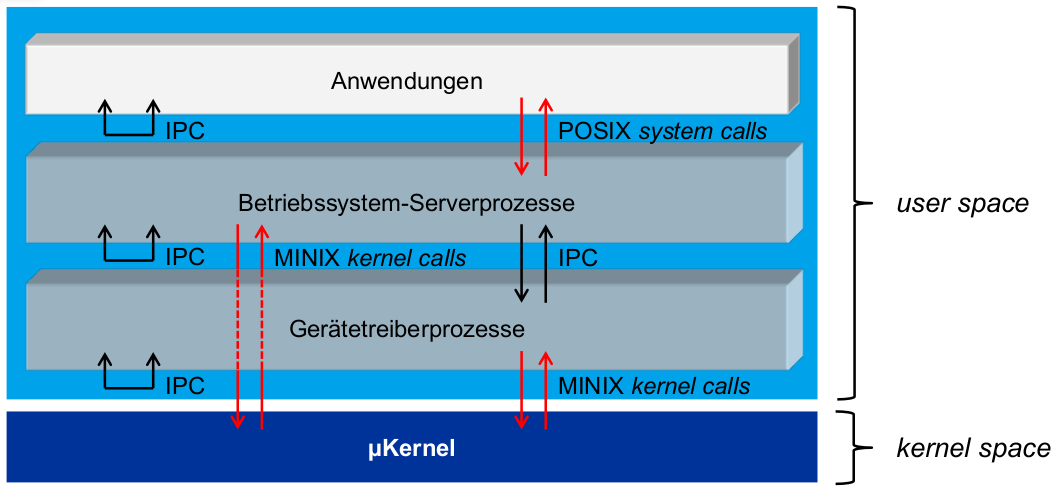
\includegraphics[width=.8\linewidth]{Assets/AdvancedOperatingSystems-minix-architektur.png}
        \item Anwendungen (weiß): Systemaufrufe im POSIX-Standard
        \item Serverprozesse (grau): IPC (botschaftenbasiert), mit Kernel: spezielle MINIX-API (kernel calls), für Anwendungsprozesse gesperrt
        %\item 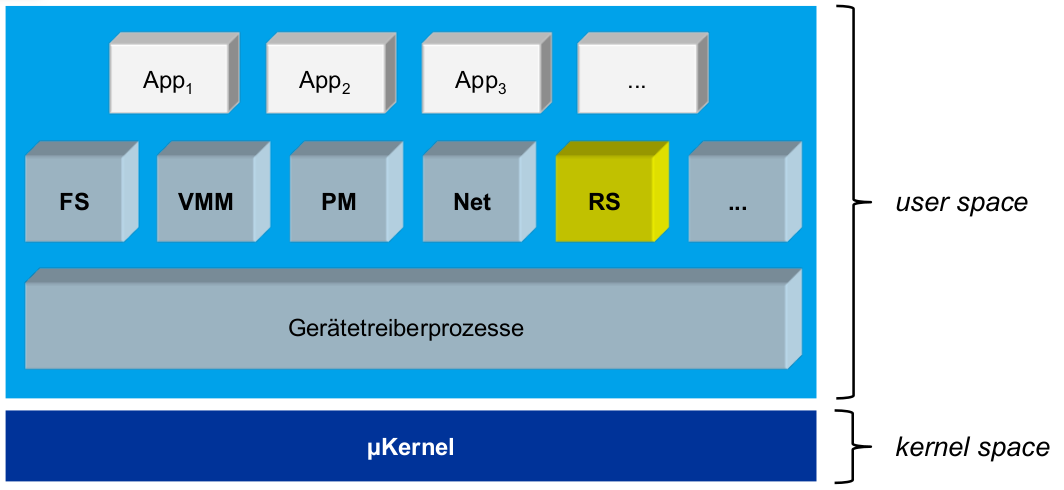
\includegraphics[width=\linewidth]{Assets/AdvancedOperatingSystems-minix-architektur-bs.png}
        \item Betriebssystem-Serverprozesse: Dateisystem (FS), Prozessmanagement (PM), Netzwerkmanagement (Net)
        \item Reincarnation Server (RS) $\rightarrow$ Micro-Reboots jeglicher Serverprozesse
        \item Kernelprozesse: systemtask, clocktask
    \end{itemize*}

    Reincarnation Server
    \begin{itemize*}
        \item Implementierungstechnik für Micro-Reboots
        \item Prozesse zum Systemstart ($\rightarrow$ Kernel Image)
        \begin{description*}
            \item[system, clock] Kernelprogramm
            \item[init] Bootstrapping (Initialisierung rs), Fork der Login-Shell
            \item[rs] Fork aller BS-Serverprozesse inkl. Gerätetreiber
        \end{description*}
        %\item 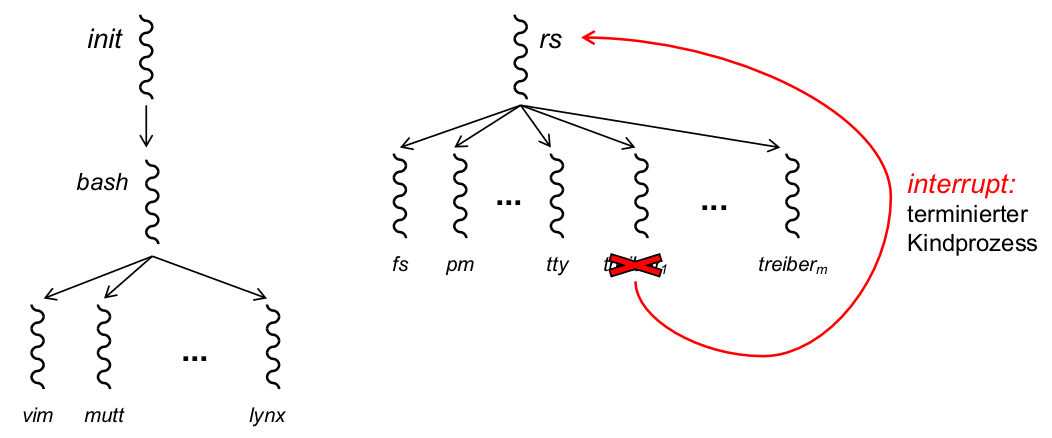
\includegraphics[width=\linewidth]{Assets/AdvancedOperatingSystems-minix-reincarnation-server.png}
    \end{itemize*}

    \subsection{Verfügbarkeit}
    \begin{itemize*}
        \item komplementäre NFE zu Robustheit: Verfügbarkeit ( availability )
        \item Verbesserung von Robustheit $\rightarrow$ Verbesserung von Verfügbarkeit
        \item Robustheitsmaßnahmen hinreichend , nicht notwendig %(hochverfügbare Systeme können sehr wohl von Ausfällen betroffen sein...)
        \item weitere komplementäre NFE: Robustheit $\rightarrow$ Sicherheit (security)
        \item Definition: Grad, zu welchem ein System oder eine Komponente funktionsfähig und zugänglich (erreichbar) ist, wann immer seine Nutzung erforderlich ist (IEEE)
        \item Anteil an Laufzeit eines Systems, in dem dieses seine spezifizierte Leistung erbringt
        %\item \includegraphics[width=\linewidth]{Assets/AdvancedOperatingSystems-verfügbarkeit-laufzeit.png}
        \item $Availability= \frac{Total Uptime}{Total Lifetime}= \frac{MTTF}{MTTF + MTTR}$
        \item MTTR: Mean Time to Recovery, MTTF: Mean Time to Failure
        \item Hochverfügbarkeitsbereich (gefeierte ,,five nines'' availability)
        \item Maßnahmen: Robustheit, Redundanz, Ausfallmanagement
    \end{itemize*}

    einige Verfügbarkeitsklassen:
    \begin{tabular}{l|l|l}
        Verfügbarkeit & Ausfallzeit pro Jahr   & Ausfallzeit pro Woche          \\\hline
        90\%          & \textgreater{} 1 Monat & ca. 17 Stunden                 \\
        99\%          & ca. 4 Tage             & ca. 2 Stunden                  \\
        99,9\%        & ca. 9 Stunden          & ca. 10 Minuten                 \\
        99,99\%       & ca. 1 Stunde           & ca. 1 Minute                   \\
        99,999\%      & ca. 5 Minuten          & ca. 6 Sekunden                 \\
        99,9999\%     & ca. 2 Sekunden         & \textless\textless{} 1 Sekunde
    \end{tabular}

    \subsubsection{QNX Neutrino: Hochverfügbares Echtzeit-BS}
    \begin{itemize*}
        \item Mikrokern-Betriebssystem
        \item primäres Einsatzfeld: eingebettete Systeme, z.B. Automobilbau
        \item Mikrokernarchitektur mit Adressraumisolation für Gerätetreiber
        \item (begrenzt) dynamische Micro-Rebootsmöglich
        \item $\rightarrow$ Maximierung der Uptime des Gesamtsystems
    \end{itemize*}
    \begin{description*}
        \item[High-Avalability-Manager] Laufzeit-Monitor der Systemdienste/Anwendungsprozesse überwacht und neustartet $\rightarrow$ $\mu$Reboot-Server
        \item[High-Availability-Client-Libraries] Funktionen zur transparenten automatischen Reboot für ausgefallene Server-Verbindungen
    \end{description*}

    \section{Sicherheit}
    Terminologie
    \begin{description*}
        \item[Security] IT-Sicherheit, Informationssicherheit
        \begin{itemize*}
            \item Ziel: Schutz \textbf{des} Rechnersystems
            \item Systemsicherheit, hier besprochen
        \end{itemize*}
        \item[Safety] Funktionale Sicherheit, Betriebssicherheit
        \begin{itemize*}
            \item Ziel: Schutz \textbf{vor} einem Rechnersystem
            \item an dieser Stelle nicht besprochen
        \end{itemize*}
    \end{description*}
    %Eine (unvollständige) Taxonomie: 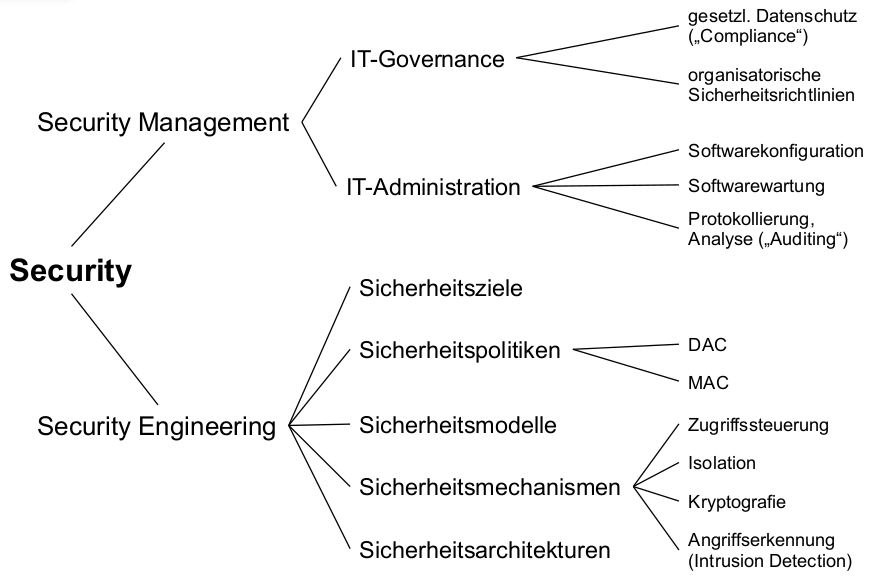
\includegraphics[width=\linewidth]{Assets/AdvancedOperatingSystems-sicherheit-taxonomie.png}

    \subsection{Sicherheitsziele}
    \begin{itemize*}
        \item Rechnersystem sicher gegen Schäden durch zielgerichtete Angriffe, insbesondere bzgl Informationen, die im System gespeichert, verarbeitet und übertragen werden
        \item für Sicherheitsziele gilt: Daten $\not=$ Informationen
        \item sukzessive Konkretisierungen bzgl anwendungsspezifischer Anforderungen
    \end{itemize*}

    abstrakte auf konkret definierte Sicherheitsziele
    \begin{description*}
        \item[Vertraulichkeit] nur für einen autorisierten Nutzerkreis zugänglich
        \item[Integrität] vor nicht autorisierter Veränderung geschützt
        \item[Verfügbarkeit] autorisierten Nutzern in angemessener Frist zugänglich
        \item[Authentizität] Urheber eindeutig erkennen
        \item[Verbindlichkeit] sowohl integer als auch authentisch
    \end{description*}

    \subsection{Schadenspotenzial}
    \begin{enumerate*}
        \item Vandalismus, Terrorismus (reine Zerstörungswut)
        \item Systemmissbrauch
        \begin{itemize*}
            \item illegitime Ressourcennutzung, hocheffektive Folgeangriffe
            \item Manipulation von Inhalten ($\rightarrow$ Desinformation)
        \end{itemize*}
        \item (Wirtschafts-) Spionage und Diebstahl
        \begin{itemize*}
            \item Verlust der Kontrolle über kritisches Wissen ($\rightarrow$ Risikotechnologien)
            \item immense wirtschaftliche Schäden, z.B. Diebstahl von industriellem Know-How
        \end{itemize*}
        \item Betrug, persönliche Bereicherung (wirtschaftliche Schäden)
        \item Sabotage, Erpressung
        \begin{itemize*}
            \item Außerkraftsetzen lebenswichtiger Infrastruktur
            \item Erpressung durch reversible Sabotage
        \end{itemize*}
    \end{enumerate*}

    \subsection{Bedrohungen}
    \begin{enumerate*}
        \item Eindringlinge (intruders), Hacker
        \begin{itemize*}
            \item Angriff nutzt technische Schwachstelle aus ( exploit )
        \end{itemize*}
        \item Schadsoftware (malicious software, malware)
        \begin{itemize*}
            \item (teil-) automatisierte Angriffe
            \item Trojanische Pferde: scheinbar nützliche Software
            \item Viren, Würmer: Funktionalität zur eigenen Vervielfältigung und/oder Modifikation
            \item Logische Bomben: trojanischen Pferde, deren Aktivierung an System- oder Datumsereignisse gebunden
            \item Root Kits
        \end{itemize*}
        \item Bots und Botnets
        \begin{itemize*}
            \item (weit-) verteilt ausgeführte Schadsoftware
            \item eigentliches Ziel i.d.R. nicht das jeweils infizierte System
        \end{itemize*}
    \end{enumerate*}

    \subsubsection{Professionelle Malware: Root  Kit}
    \begin{itemize*}
        \item Programm-Paket, das unbemerkt Betriebssystem modifiziert, um Administratorrechte zu erlangen
        \item Voraussetzung: eine einzige Schwachstelle...
        \item ermöglichen Zugriff auf alle Funktionen und Dienste eines Betriebssystems
        \item Angreifer erlangt vollständige Kontrolle des Systems und kann
        \begin{itemize*}
            \item Dateien (Programme) hinzufügen bzw. ändern
            \item Prozesse überwachen
            \item über die Netzverbindungen senden und empfangen
            \item Hintertüren für zukünftiger Angriffe platzieren
        \end{itemize*}
        \item Ziele eines Rootkits
        \begin{itemize*}
            \item seine Existenz verbergen
            \item zu verbergen, welche Veränderungen vorgenommen wurden
            \item vollständige und irreversible Kontrolle über BS zu erlangen
        \end{itemize*}
        \item erfolgreicher Root-Kit-Angriff ...
        \begin{itemize*}
            \item jederzeit, unentdeckbar, nicht reversibel
            \item systemspezifischem Wissen über Schwachstellen
            \item vollautomatisiert, also reaktiv unverhinderbar
            \item uneingeschränkte Kontrolle über Zielsystem erlangen
        \end{itemize*}
    \end{itemize*}

    \subsubsection{Schwachstellen}
    \begin{enumerate*}
        \item Passwort (erraten, zu einfach, Brute-Force, Abfangen)
        \item Programmierfehler (Speicherfehler in Anwenderprogrammen/Gerätemanagern/Betriebssystem
        \item Mangelhafte Robustheit
        \begin{itemize*}
            \item keine Korrektur fehlerhafter Eingaben
            \item buffer overrun/underrun (,,Heartbleed'')
        \end{itemize*}
        \item Nichttechnische Schwachstellen
        \begin{itemize*}
            \item physisch, organisatorisch, infrastrukturell
            \item menschlich ( $\rightarrow$ Erpressung, socialengineering )
        \end{itemize*}
    \end{enumerate*}

    \subsubsection{Zwischenfazit}
    \begin{itemize*}
        \item Schwachstellen sind unvermeidbar
        \item Bedrohungen sind unkontrollierbar
        \item ... und nehmen tendeziell zu!
        \item führt zu operationellen Risiken beim Betrieb eines IT-Systems
        \item[$\rightarrow$] Aufgabe der BS-Sicherheit: Auswirkungen operationeller Risiken reduzieren
    \end{itemize*}

    \subsection{Sicherheitspolitiken}
    \begin{itemize*}
        \item Herausforderung: korrekte Durchsetzung von Sicherheitspolitiken
        \item Vorgehensweise: Security Engineering
    \end{itemize*}
    \begin{description}
        \item[Sicherheitsziele] Welche Sicherheitsanforderungen muss BS erfüllen?
        \item[Sicherheitspolitik] Durch welche Strategien soll es diese erfüllen?
        \item[Sicherheitsmechanismen] Wie implementiert BS Sicherheitspolitik?
        \item[Sicherheitsarchitektur] Wo implementiert BS S.-mechanismen?
    \end{description}

    \subsubsection{Sicherheitspolitiken und -modelle}
    Kritisch für korrekten Entwurf, Spezifikation, Implementierung
    \begin{itemize*}
        \item Sicherheitspolitik (Policy): Menge von Regeln, zum Erreichen eines Sicherheitsziels
        \item Sicherheitsmodell: formale Darstellung zur
        \begin{itemize*}
            \item Verifikation ihrer Korrektheit
            \item Spezifikation ihrer Implementierung
        \end{itemize*}
    \end{itemize*}

    \subsubsection{Zugriffssteuerungspolitiken}
    \begin{description*}
        \item[Zugriffssteuerung] (access control) Steuerung, welcher Nutzer oder Prozess mittels welcher Operationen auf welche BS-Ressourcen zugreifen darf
        \item[Zugriffssteuerungspolitik] konkrete Regeln, welche die Zugriffssteuerung in einem BS beschreiben
        \item[IBAC] (Identity-based AC) Politik spezifiziert, welcher Nutzer an welchen Ressourcen bestimmte Rechte hat
        \begin{itemize*}
            \item Bsp.: ,,Nutzer Anna darf Brief.docx lesen''
        \end{itemize*}
        \item[TE] (Type-Enforcement) Politik spezifiziert Rechte durch zusätzliche Abstraktion (Typen): welcher Nutzertyp an welchem Ressourcentyp bestimmte Rechte hat
        \begin{itemize*}
            \item Bsp.: ,,Nutzer vom Typ Administrator darf...''
        \end{itemize*}
        \item[MLS] (Multi-Level Security) Politik spezifiziert Rechte, indem aus Nutzern und Ressourcen hierarchische Klassen (Ebenen, ,,Levels'') gleicher Kritikalität im Hinblick auf Sicherheitsziele gebildet werden
        \begin{itemize*}
            \item Bsp.: ,,Nutzer der Klasse nicht vertrauenswürdig...''
        \end{itemize*}
        \item[DAC] (Discretionary AC): Aktionen der Nutzer setzen die Sicherheitspolitik durch. Typisch: Begriff des Eigentümers von BS-Ressourcen
        \begin{itemize*}
            \item Bsp.: ,,Der Eigentümer einer Datei ändert...''
        \end{itemize*}
        \item[MAC] (Mandatory AC, obligatorische Zugriffssteuerung) Keine Beteiligung der Nutzer an der Durchsetzung einer (zentral administrierten) Sicherheitspolitik
        \begin{itemize*}
            \item Bsp.: ,,Anhand des Dateisystempfads bestimmt BS...''
        \end{itemize*}
    \end{description*}

    \subsubsection{Traditionell: DAC, IBAC}
    Auszug aus der Unix-Sicherheitspolitik:
    \begin{itemize*}
        \item es gibt Subjekte (Nutzer/Prozesse) und Objekte (Dateien,\dots)
        \item jedes Objekt hat einen Eigentümer
        \item Eigentümer legen Zugriffsrechte an Objekten fest ($\rightarrow$ DAC)
        \item es gibt drei Zugriffsrechte: read, write, execute
        \item je Objekt gibt es drei Klassen von Subjekten, mit individuellen Zugriffsrechten: Eigentümer, Gruppe, Rest
    \end{itemize*}

    In der Praxis
    \begin{itemize*}
        \item identitätsbasierte (IBAC), wahlfreie Zugriffssteuerung (DAC)
        \item hohe individuelle Freiheit der Nutzer bei Durchsetzung der Politik
        \item hohe Verantwortung
    \end{itemize*}

    \subsubsection{Modellierung: Zugriffsmatrix}
    \begin{itemize*}
        \item Access Control Matrix (acm): Momentaufnahme der globalen Rechteverteilung zu einem definierten Zeitpunkt t
        \item Korrektheitskriterium: Wie kann sich dies nach t möglicherweise ändern...?
        \item Rechteausbreitung (privilege escalation): verursacht z.B. durch Nutzeraktion ($\rightarrow$ DAC)
        \item Sicherheitseigenschaft: HRU Safety $\rightarrow$ Systemsicherheit
    \end{itemize*}

    \subsubsection{Modern: MAC, MLS}
    Sicherheitspolitik der Windows UAC (user account control)
    \begin{itemize*}
        \item es gibt Subjekte (Prozesse) und Objekte (Dateisystemknoten)
        \item jedem Subjekt ist eine Integritätsklasse zugewiesen:
        \begin{description*}
            \item[Low] nicht vertrauenswürdig
            \item[Medium] reguläre Nutzerprozesse, die Nutzerdaten manipulieren
            \item[High] Administratorprozesse, die Systemdaten manipulieren
            \item[System] (Hintergrund-) Prozesse, die ausschließlich Betriebssystemdienste auf Anwenderebene implementieren
        \end{description*}
        \item jedem Objekt ist analog eine dieser Integritätsklassen zugewiesen
        \item sämtliche DAC-Zugriffsrechte müssen mit einer Hierarchie der Integritätsklassen konsistent sein ( $\rightarrow$ MAC)
        \item Nutzer können Konsistenzanforderung selektiv außer Kraft setzen ($\rightarrow$ DAC)
    \end{itemize*}

    MAC-Modellierung: Klassenhierarchie

    Beispiel Relation: $\leq=\{(High,Medium), (High,Low), (Medium,Low), (High,High), (Low,Low)\}$
    \begin{itemize*}
        \item repräsentiert Kritikalität hinsichtlich der Integrität
        \item modelliert legale Informationsflüsse zwischen Subjekten und Objekten $\rightarrow$ Schutz vor illegalem Überschreiben
        \item leitet Zugriffsrechte aus Informationsflüssen ab: lesen/schreiben
    \end{itemize*}

    %\subparagraph{DAC-Modellierung: Zugriffsmatrix}
    %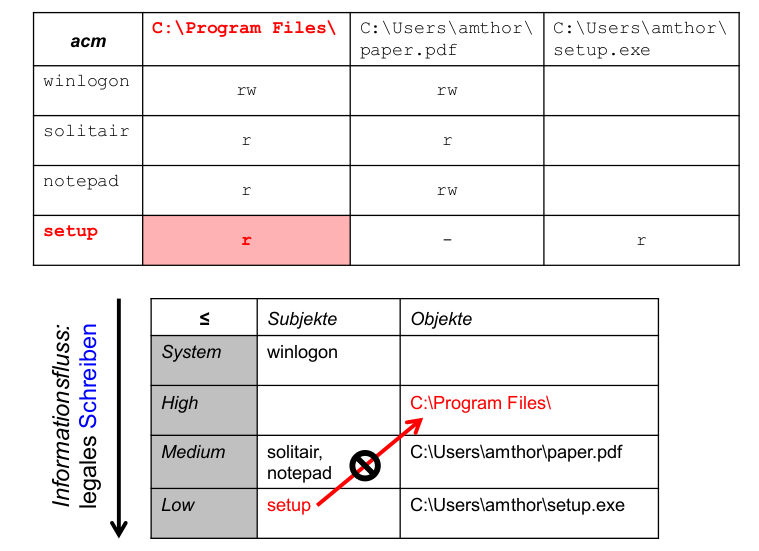
\includegraphics[width=\linewidth]{Assets/AdvancedOperatingSystems-dac-zugriffsmatrix.png}

    \subparagraph{Modellkorrektheit: Konsistenz}
    \begin{itemize*}
        \item Korrektheitskriterium: Garantiert die Politik, dass acm mit $\leq$ jederzeit konsistent ist? ( BLP Security )
        \item elevation-Mechanismus: verändert nach Nutzeranfrage ($\rightarrow$ DAC) sowohl acm als auch $\leq\rightarrow$ konsistenzerhaltend?
        \item anders: verändern unmittelbar nur acm $\rightarrow$ konsistenzerhaltend?
    \end{itemize*}

    \subsection{Autorisierungsmechanismen}
    \begin{itemize*}
        \item Sicherheitsmechanismen: Datenstrukturen und Algorithmen, welche Sicherheitseigenschaften eines BS implementieren
        \item[$\rightarrow$] Sicherheitsmechanismen benötigt man zur Herstellung jeglicher Sicherheitseigenschaften
        \item Auswahl im Folgenden: Autorisierungsmechanismen und -informationen
        \begin{itemize*}
            \item Nutzerauthentisierung (Passwort-Hashing, ...)
            \item Autorisierungsinformationen (Metainformationen...)
            \item Autorisierungsmechanismen (Rechteprüfung, ...)
            \item kryptografische Mechanismen (Hashfunktionen, ...)
        \end{itemize*}
    \end{itemize*}

    \subsubsection{Traditionell: ACLs, SUID}
    Autorisierungsinformationen:
    \begin{itemize*}
        \item müssen Subjekte (Nutzer) bzw. Objekte (Dateien, Sockets ...) mit Rechten assoziieren $\rightarrow$ Implementierung der Zugriffsmatrix (acm), diese ist:
        \begin{itemize*}
            \item groß ($\rightarrow$ Dateianzahl auf Fileserver)
            \item dünn besetzt
            \item in Größe und Inhalt dynamisch veränderlich
        \end{itemize*}
        \item Lösung: verteilte Implementierung der acm als Spaltenvektoren, deren Inhalt in den Objekt-Metadaten repräsentiert wird: Zugriffssteuerungslisten (ACLs)
    \end{itemize*}

    \subparagraph{ACLs: Linux-Implementierung}
    \begin{itemize*}
        \item objektspezifischer Spaltenvektor = Zugriffssteuerungsliste
        \item Dateisystem-Metainformationen: implementiert in I-Nodes
    \end{itemize*}

    Modell einer Unix acm ...
    \begin{tabular}{c|c|c|c}
                       & lesen & schreiben & ausführen \\\hline
        Eigentümer (u) & ja    & ja        & ja        \\
        Gruppe (g)     & ja    & nein      & ja        \\
        Rest (o)       & ja    & nein      & ja
    \end{tabular}
    \begin{itemize*}
        \item 3-elementige Liste, 3-elementige Rechtemenge
        \item[$\rightarrow$] 9 Bits
        \item Implementierung kodiert in 16-Bit-Wort: 1 1 1 1 0 1 1 0 1
    \end{itemize*}

    \subparagraph{Autorisierungsmechanismen: ACL-Auswertung}
    Subjekte = Nutzermenge besteht aus Anzahl registrierter Nutzer
    \begin{itemize*}
        \item jeder hat eindeutige UID (userID), z.B. integer- Zahl
        \item Dateien \& Prozesse mit UID des Eigentümers versehen
        \begin{itemize*}
            \item bei Dateien: Teil des I-Nodes
            \item bei Prozessen: Teil des PCB
            \item standardmäßiger Eigentümer: der Ressource erzeugt hat
        \end{itemize*}
    \end{itemize*}

    Nutzergruppen (groups)
    \begin{itemize*}
        \item jeder Nutzer durch Eintrag in Systemdatei (/etc/group) einer/mehreren Gruppen zugeordnet ($\rightarrow$ ACL: g Rechte)
    \end{itemize*}

    Superuser oder root... hat grundsätzlich uneingeschränkte Rechte.
    \begin{itemize*}
        \item UID = 0
        \item darf alle Dateien im System lesen, schreiben, ausführen
        \item unabhängig von ACL
    \end{itemize*}

    \subparagraph{ACL-Implementierung}
    Nutzerrechte $\rightarrow$ Prozessrechte

    Durchsetzung: basiert auf Prozessrechten
    \begin{itemize*}
        \item Annahme: Prozesse laufen mit UID des Nutzers, der sie gestartet hat und repräsentieren Nutzerberechtigungen
        \item technisch: Nutzer beauftragt anderen Prozess, sich zu dublizieren (fork()) und gewünschte Programm auszuführen (exec*())
        \item Vererbungsprinzip %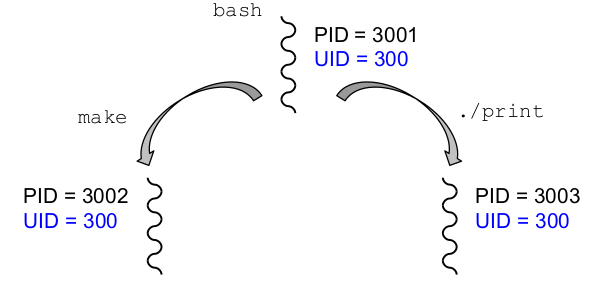
\includegraphics[width=\linewidth]{Assets/AdvancedOperatingSystems-acl-vererbungsprinzip.png}
    \end{itemize*}

    \subparagraph{Autorisierungsmechanismen: Set-UID}

    konsequente Rechtevererbung
    \begin{itemize*}
        \item Nutzer können im Rahmen der DAC-Politik ACLs manipulieren
        \item Nutzer können (i.A.) jedoch keine Prozess-UIDs manipulieren
        \item $\rightarrow$ und genau so sollte es gem. Unix-Sicherheitspolitik auch sein!
    \end{itemize*}

    Hintergrund
    \begin{itemize*}
        \item Unix-Philosophie ,, everything is a file '': BS-Ressourcen wie Sockets, E/A-Gerätehandler als Datei repräsentiert $\rightarrow$ identische Schutzmechanismen zum regulären Dateisystem
        \item somit: Autorisierungsmechanismen zur Begrenzung des Zugriffs auf solche Geräte nutzbar
        \begin{itemize*}
            \item \emph{root} bzw. zweckgebundener Nutzer muss Eigentümer sein
            \item ACL als \texttt{rw-\ ---\ ---} gesetzt sein
            \item[$\rightarrow$] Nutzerprozesse könnten z.B. nicht drucken ...
        \end{itemize*}
        \item Lösung: Mechanismus zur Rechtedelegation
        \begin{itemize*}
            \item durch weiteres Recht in ACL: SUID-Bit (setUID)
            \item Programmausführung modifiziert Kindprozess, so dass UID des Programmeigentümers seine Rechte bestimmt
            \item Technik: von UID abweichende Prozess-Metainformation ($\rightarrow$ PCB) effektive UID (eUID) wird tatsächlich zur Autorisierung genutzt
        \end{itemize*}
    \end{itemize*}

    Strategie für sicherheitskritische Linux-Programme
    \begin{itemize*}
        \item Eigentümer \emph{root}, SUID-Bit gesetzt
        \item per eUID delegiert root seine Rechte an genau solche Kindprozesse, die  SUID-Programme ausführen
        \item[$\rightarrow$] Nutzerprozesse können Systemprogramme ohne permanente root-Rechte ausführen
    \end{itemize*}

    Weiteres Beispiel: passwd
    \begin{itemize*}
        \item ermöglicht Nutzern Ändern des (eigenen) Anmeldepassworts
        \item Schreibzugriff auf /etc/shadow (Password-Hashes) erforderlich
        \item Lösung: `-rws rws r-x 1 root root 1 2005-01-20 10:00 passwd\$
        \item passwd-Programm wird mit root-Rechten ausgeführt und passwd schreibt nur eigenen Passwort-Hash
    \end{itemize*}

    \subsection{Modern: SELinux}
    \begin{itemize*}
        \item 2000er: sicherheitsfokussiertes Betriebssystemprojekt für NSA
        \item Implementierung des $\mu$Kernel-Architekturkonzepts Flask
        \item heute: Open Source, Teil des mainline Linux Kernels
        \item Klassische UNIXoide: Sicherheitspolitik fest im Kernel
        \item Idee SELinux: Sicherheitspolitikals eigene BS-Abstraktion
        \begin{itemize*}
            \item zentrale Datenstruktur für Regeln, die erlaubte Zugriffe auf ein SELinux-System definiert
            \item erlaubt Modifikation und Anpassung an verschiedene Sicherheitsanforderungen $\rightarrow$ NFE Adaptivität ...
        \end{itemize*}
    \end{itemize*}

    BS-Komponenten
    \begin{itemize*}
        \item Auswertung: Security-Server, implementiert als Linux-Kernelmodul $\rightarrow$ entscheidet über alle Zugriffe auf alle Objekte
        \item Durchsetzung der Sicherheitspolitik: LSM Hooks
        \item Administration: geschrieben in Textform, muss zur Laufzeit in Security Server installiert werden
    \end{itemize*}
    %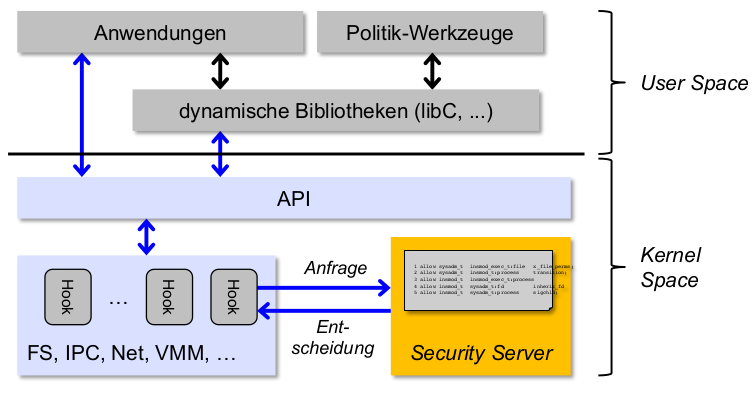
\includegraphics[width=\linewidth]{Assets/AdvancedOperatingSystems-selinux-security-server.png}
    %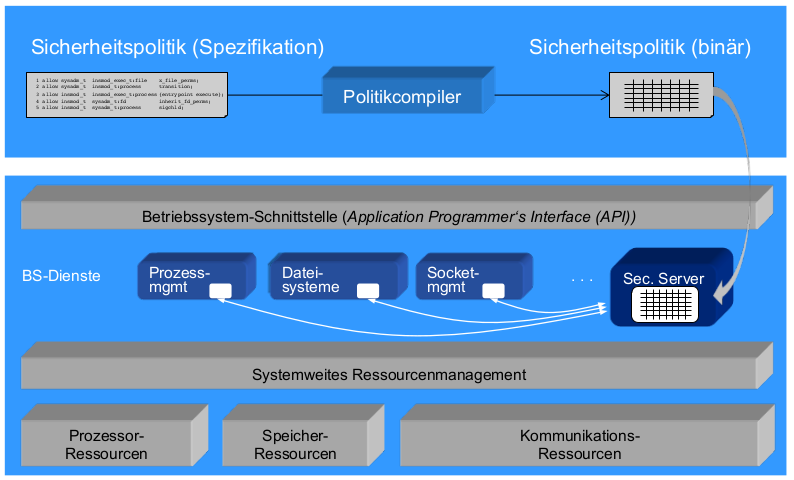
\includegraphics[width=\linewidth]{Assets/AdvancedOperatingSystems-selinux-sicherheitspolitik-installieren.png}

    Repräsentation der Sicherheitspolitik
    \begin{itemize*}
        \item physisch: in spezieller Datei, die alle Regeln enthält, die der Kernel durchsetzen muss
        \item Datei wird aus Menge von Quelldateien in einer Spezifikationssprache für SELinux-Sicherheitspolitiken kompiliert
        \item ermöglicht anforderungsspezifische SELinux-Politiken: können sich von SELinux-System zum anderen wesentlich unterscheiden
        \item Politik wird während des Boot-Vorgangs in Kernel geladen
    \end{itemize*}

    Semantische Konzepte (Auswahl)
    \begin{itemize*}
        \item Type Enforcement (TE): Typisierung von
        \begin{itemize*}
            \item Subjekten: Prozesse
            \item Objekten der Klassen: Dateien, Sockets, Geräteschnittstellen, ...
        \end{itemize*}
        \item Rechte delegation durch Retypisierung (vgl. Unix-SUID)
        %\item 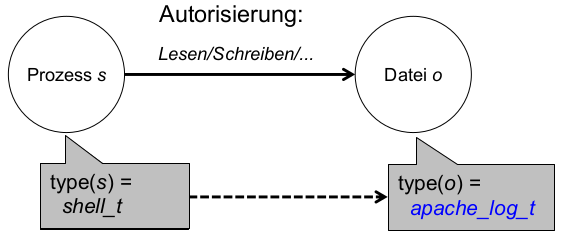
\includegraphics[width=\linewidth]{Assets/AdvancedOperatingSystems-selinux-retypisierung.png}
    \end{itemize*}

    \subparagraph{Autorisierungsinformationen}
    Security Context: Respräsentiert SELinux-Autorisierungsinformationen für jedes Objekt (Semantik: Prozess bash läuft mit Typ \texttt{shell\_t})

    \subparagraph{Autorisierungsregeln}
    ... werden systemweit festgelegt in dessen Sicherheitspolitik ($\rightarrow$ MAC)

    Access Vector Rules
    \begin{itemize*}
        \item Autorisierungsregeln basierend auf Subjek-/Objekttypen
        \item Zugriffe müssen explizit gewährt werden (default-deny)
        %\begin{Shaded}
        %\begin{Highlighting}[]
        %\ExtensionTok{allow}\NormalTok{ shell_t passwd_exec_t : file \{ execute \};}
        %\ExtensionTok{allow}\NormalTok{ passwd_t shadow_t : file \{ read write \};}
        %\end{Highlighting}
        %\end{Shaded}
        \item Semantik: Erlaube (''allow'') ...
        \begin{itemize*}
            \item jedem Prozess mit Typ \texttt{shell\_t}
            \item ausführenden Zugriff (benötigt die Berechtigung \texttt{execute})
            \item auf Dateien (also Objekte der Klassefile)
            \item mit Typ \texttt{passwd\_exec\_t}
        \end{itemize*}
    \end{itemize*}

    \subparagraph{Autorisierungsmechanismen: passwd Revisited}
    \begin{itemize*}
        \item Lösung: Retypisierung bei Ausführung
        \item Prozess wechselt in einen aufgabenspezifischen Typ \texttt{passwd\_t}
        \item[$\rightarrow$] massiv verringertes Missbrauchspotenzial!
        %\item \includegraphics[width=\linewidth]{Assets/AdvancedOperatingSystems-passwd-lösung2.png}
    \end{itemize*}

    SELinux: weitere Politiksemantiken
    \begin{itemize*}
        \item hier gezeigt: Überblick über TE
        \item außerdem relevant für SELinux-Politiken (und deren Administration)
        \begin{itemize*}
            \item Einschränkung von erlaubten Typtransitionen (Welches Programm darf mit welchem Typ ausgeführt werden?)
            \item weitere Abstraktionsschicht: rollenbasierte Regeln (RBAC)
            \item[$\rightarrow$] Schutz gegen nicht vertrauenswürdige Nutzer
        \end{itemize*}
        \item[\cmark] extrem feingranulare, anwendungsspezifische Sicherheitspolitik zur Vermeidung von privilege escalation Angriffen
        \item[\cmark] obligatorische Durchsetzung ( $\rightarrow$ MAC, zusätzlich zu DAC)
        \item[O] Softwareentwicklung: Legacy-Linux-Anwendungen ohne Einschränkung
        \item[\xmark] Politikentwicklung und -administration komplex
        \item[$\rightarrow$] MAC-Mechanismen ala SELinux sind heutzutage in vielerlei Software bereits zu finden
    \end{itemize*}

    \subsection{Isolationsmechanismen}
    \begin{itemize*}
        \item bekannt: Isolationsmechanismen für robuste Betriebssysteme
        \begin{itemize*}
            \item strukturierte Programmierung
            \item Adressraumisolation
        \end{itemize*}
        \item nun: Isolationsmechanismen für sichere Betriebssysteme
        \begin{itemize*}
            \item krypto. Hardwareunterstützung: Intel SGX Enclaves
            \item sprachbasiert:
            \begin{itemize*}
                \item streng typisierte Sprachen und \emph{managed code}: Microsoft Singularity
                \item speichersichere Sprachen (Rust) + Adressraumisolation ($\mu$Kernel): \href{https://www.redox-os.org/}{RedoxOS}
            \end{itemize*}
            \item isolierte Laufzeitumgebungen: Virtualisierung
        \end{itemize*}
    \end{itemize*}

    \subsubsection{Intel SGX}
    \begin{itemize*}
        \item SGX: Software Guard Extensions
        \item Ziel: Schutz von sicherheitskritischen Anwendungen durch vollständige, hardwarebasierte Isolation
        \item $\rightarrow$ strenggenommen kein BS-Mechanismus: Anwendungen müssen dem BS nicht mehr vertrauen
        \item Annahmen/Voraussetzungen
    \end{itemize*}
    \begin{enumerate*}
        \item sämtliche Software nicht vertrauenswürdig (potenziell durch Angreifer kontrolliert)
        \item Kommunikation mit dem angegriffenen System nicht vertrauenswürdig (weder vertraulich noch verbindlich)
        \item kryptografische Algorithmen (Verschlüsselung und Signierung) sind vertrauenswürdig, also nicht für den Angreifer zu brechen
        \item Ziel: Vertraulichkeit, Integrität und Authentizität von Anwendungen und durch sie verarbeiteten Informationen
    \end{enumerate*}

    \subparagraph{Enclaves}
    \begin{itemize*}
        \item Idee: geschützter Speicherbereich für Teilmenge der Seiten (Code und Daten) einer Task: Enclave Page Cache (EPC)
        \item Prozessor ver-und entschlüsselt EPC-Seiten
        %\item 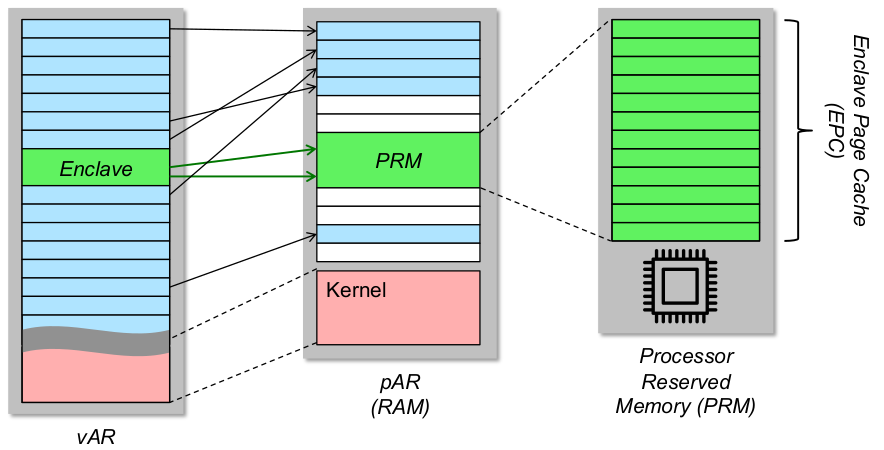
\includegraphics[width=\linewidth]{Assets/AdvancedOperatingSystems-SGX-enclaves.png}
    \end{itemize*}
    \begin{description*}
        \item[ECREATE] App $\rightarrow$ Syscall $\rightarrow$ BS-Instruktion an CPU
        \item[EADD] App $\rightarrow$ Syscall $\rightarrow$ BS-Instruktion an CPU
        \begin{itemize*}
            \item Metainformationen für jede hinzugefügte Seite als Teil der EPC-Datenstruktur
        \end{itemize*}
        \item[EINIT] App. $\rightarrow$ Syscall $\rightarrow$ BS-Instruktion an CPU
        \begin{itemize*}
            \item finalisiert gesamten Speicherinhalt für diese Enclave
            \item CPU erzeugt Hashwert = eindeutige Signatur des Enclave - Speicherinhalts
            %\item falls BS bis zu diesem Punkt gegen Integrität der Anwendung verstoßen hat: durch Vergleich mit von dritter Seite generiertem Hashwert feststellbar!
        \end{itemize*}
    \end{description*}
    \begin{center}
        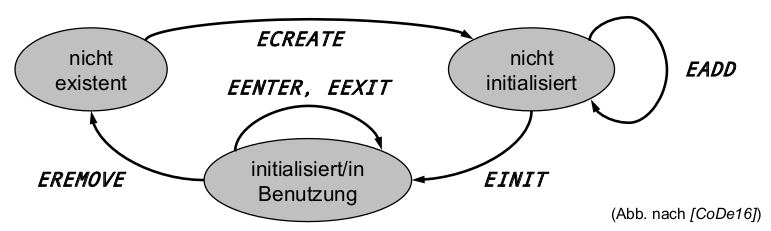
\includegraphics[width=.6\linewidth]{Assets/AdvancedOperatingSystems-SGX-enclaves-model.png}
    \end{center}
    \begin{itemize*}
        \item Zugriff: App $\rightarrow$ CPU-Instruk. in User Mode (EENTER, EEXIT)
        \item CPU erfordert, dass EPC-Seiten in vAR der zugreifenden Task
        %\item 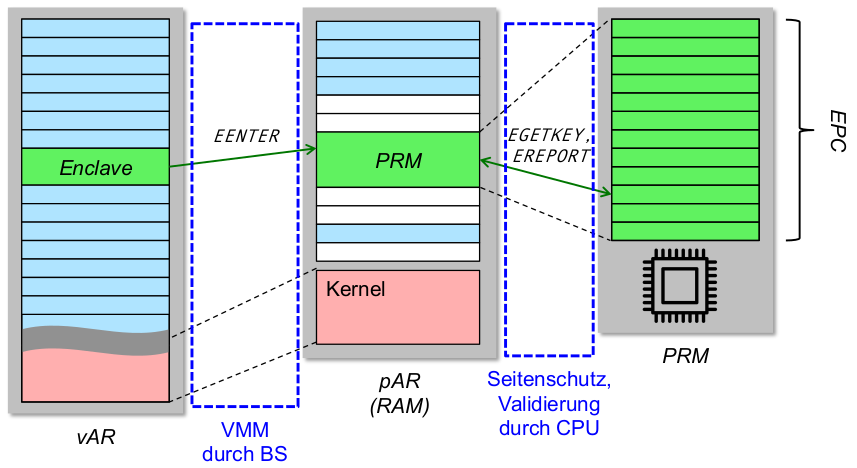
\includegraphics[width=\linewidth]{Assets/AdvancedOperatingSystems-SGX-enlaves-zugriff.png}
    \end{itemize*}

    \subparagraph{SGX: Licht und Schatten}
    \begin{itemize*}
        \item Einführung 2015 in Skylake - Mikroarchitektur
        \item seither in allen Modellen verbaut, jedoch nicht immer aktiviert
        \item Konzept hardwarebasierter Isolation ...
        \item[\cmark] liefert erstmals die Möglichkeit zur Durchsetzung von Sicherheitspolitiken auf Anwendungsebene
        \item[O]setzt Vertrauen in korrekte (und nicht böswillige) Hardwarevoraus
        \item[O]Dokumentation und Entwicklerunterstützung (im Ausbau ...)
        \item[\xmark] schützt durch Enclaves einzelne Anwendungen aber nicht System
        \item[\xmark] steckt in praktischer Eigenschaften (Performanz, Speicher) noch in den Anfängen
    \end{itemize*}

    \subsection{Sicherheitsarchitekturen}
    \begin{itemize*}
        \item Voraussetzung zum Verstehen jeder Sicherheitsarchitektur
        \begin{itemize*}
            \item Verstehen des Referenzmonitorprinzips
            \item frühe Forschungen durch US-Verteidigungsministerium
            \item Schlüsselveröffentlichung: Anderson-Report (1972)
            \item[$\rightarrow$] fundamentalen Eigenschaften zur Charakterisierung von Sicherheitsarchitekturen
        \end{itemize*}
        \item Begriffe des Referenzmonitorprinzips kennen wir schon
        \begin{itemize*}
            \item Abgrenzung passiver Ressourcen (Objekte, z.B. Dateien)
            \item von Subjekten (aktiven Elementen, Prozess) durch BS
        \end{itemize*}
    \end{itemize*}

    \subsubsection{Referenzmonitorprinzip}
    \begin{itemize*}
        \item[$\rightarrow$] sämtliche Autorisierungsentscheidungen durch zentralen Mechanismus = Referenzmonitor
        \item Bewertet jeden Zugriffsversuch eines Subjekts auf Objekt durch Anwendung einer Sicherheitspolitik (security policy)
        \item Architekturbeschreibung, wie Zugriffe auf Ressourcen, die Sicherheitspolitik erlaubt, eingeschränkt werden
        \item Autorisierungsentscheidungen: basieren auf sicherheitsrelevanten Eigenschaften jedes Subjekts und jedes Objekts
        %\item 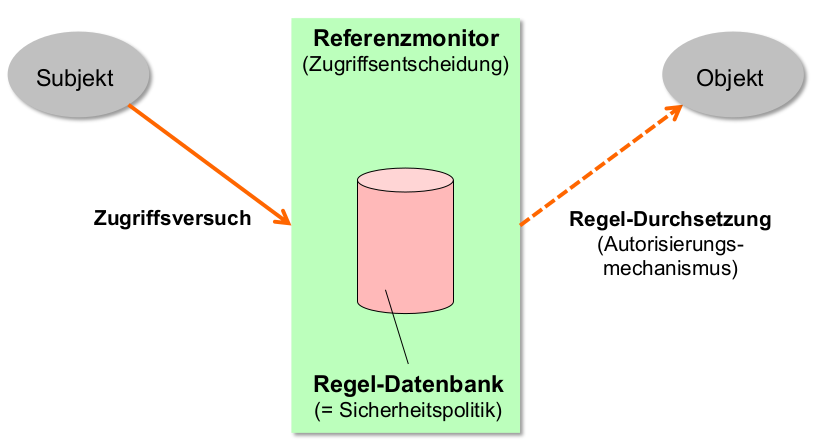
\includegraphics[width=\linewidth]{Assets/AdvancedOperatingSystems-Referenzmonitorprinzip.png}
    \end{itemize*}

    Referenzmonitor ist eine Architekturkomponenten, die
    \begin{description*}
        \item[RM 1] bei sämtlichen Subjekt/Objekt-Interaktionen involviert sind $\rightarrow$ Unumgehbarkeit (total mediation)
        \item[RM 2] geschützt sind vor unautorisierter Manipulation $\rightarrow$ Manipulationssicherheit (tamperproofness)
        \item[RM 3] hinreichend klein und wohlstrukturiert sind, für formale Analysemethoden $\rightarrow$ Verifizierbarkeit (verifyability)
    \end{description*}

    \subparagraph{Referenzmonitor in Betriebssystemen}
    Nahezu alle Betriebssysteme implementieren irgendeine Form eines Referenzmonitors
    \begin{itemize*}
        \item Subjekte, Objekte
        \item Regeln einer Sicherheitspolitik charakterisiert
        \item Unumgehbarkeit, Manipulationssicherheit
        \item Verifizierbarkeit ihrer Sicherheitsarchitektur
    \end{itemize*}

    Beispiel: Standard-Linux
    \begin{itemize*}
        \item Subjekte (Prozesse) $\rightarrow$ haben reale Nutzer-Identifikatoren (UIDs)
        \item Objekte (Dateien) $\rightarrow$ haben ACLs (,,rwxrw----'')
        \item Regeln der Sicherheitspolitik $\rightarrow$ hart codiert, starr
        \item Sicherheitsattribute, $\rightarrow$ Objekten zugeordnet, modifizierbar
    \end{itemize*}
    Man beurteile die Politikimplementierung in dieser Architektur bzgl. Unumgehbarkeit, Manipulationssicherheit und Verifizierbarkeit

    Referenzmonitorimplementierung: Flask
    \begin{center}
        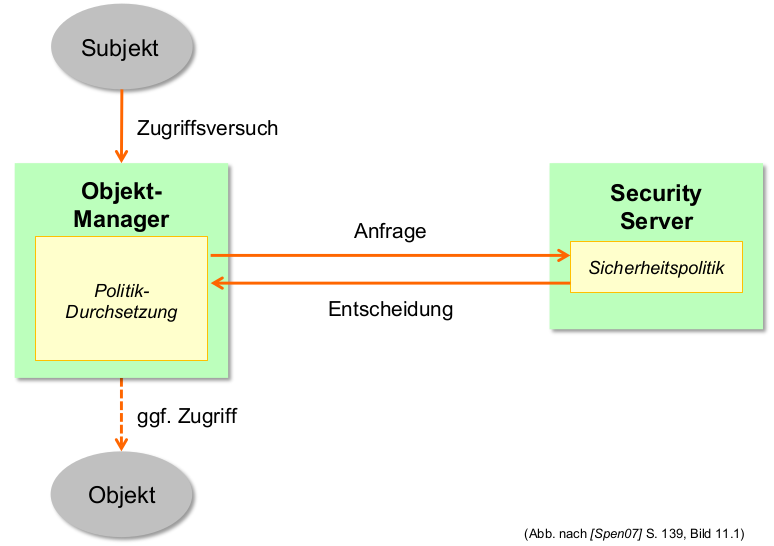
\includegraphics[width=.5\linewidth]{Assets/AdvancedOperatingSystems-referenzmonitor-flask.png}
    \end{center}

    \subparagraph{SELinux-Architektur: Security Server}
    \begin{itemize*}
        \item Security Server: Laufzeitumgebung für Politik in Schutzdomäne des Kerns
        \item Objektmanager: implementiert in allen BS-Diensten mittels ,,Linux Security Module Framework ''
        \item Objektmanager zur Verwaltung verschiedener Objektklassen
        \item spiegeln Diversität und Komplexität von Linux BS-Abtraktionen wider: Dateisysteme, Netzwerk, IPC, ...
        \item jedes Subsystem von SELinux zuständig für
        \begin{enumerate*}
            \item Erzeugung neuer Objekte
            \item Zugriff auf existierende Objekte
        \end{enumerate*}
        \item Beispiele: Prozess-Verwaltung, Dateisystem, Networking-System
    \end{itemize*}

    Dateisystem als Objektmanager
    \begin{itemize*}
        \item Durch Analyse von Linux - Dateisystem und zugehöriger API wurden zu überwachenden Objektklassen identifiziert
        \item ergibt sich unmittelbar aus Linux-API: Dateien, Verzeichnisse, Pipes
        \item feingranularere Objektklassen für durch Dateien repräsentierte Objekte (Unix: ,,everything is a file'')
    \end{itemize*}

    Permissions (Zugriffsrechte)
    \begin{itemize*}
        \item für jede Objektklasse: Menge an Permissions definiert, um Zugriffe auf Objekte dieser Klasse zu kontrollieren
        \item Permissions: abgeleitet aus Dienstleistungen, die Linux-Dateisystem anbietet
        \item[$\rightarrow$] Objektklassen gruppieren verschiedene Arten von Zugriffsoperationen auf verschiende Arten von Objekten
        \item z.B. Permissions für alle ,,Datei''-Objektklassen (Auswahl ...)
    \end{itemize*}

    \subsubsection{Trusted Computing Base (TCB)}
    Begriff zur Bewertung von Referenzmonitorarchitekturen
    \begin{itemize*}
        \item[=] notwendige Hard-und Softwarefunktionen eines IT-Systems um alle Sicherheitsregeln durchzusetzen
        \item besteht üblicherweise aus
        \begin{enumerate*}
            \item Laufzeitumgebung der Hardware (nicht E/A-Geräte)
            \item verschiedenen Komponenten des Betriebssystem-Kernels
            \item Benutzerprogrammen mit sicherheitsrelevanten Rechten
        \end{enumerate*}
        \item Betriebssystemfunktionen, die Teil der TCB sein müssen, beinhalten Teile des Prozess-, Speicher-, Datei-, E/A-Managements
    \end{itemize*}

    \section{Echtzeitfähigkeit}
    Jedes System, bei dem der Zeitpunkt, zu dem der Output erzeugt wird, von Bedeutung ist. Dies liegt in der Regel daran, dass die Eingabe einer Bewegung in der physischen Welt entspricht und die Ausgabe sich auf dieselbe Bewegung beziehen muss. Die Verzögerung zwischen Eingabe- und Ausgabezeit muss für eine akzeptable Aktualität ausreichend klein sein.

    Spektrum von Echtzeitsystemen
    \begin{enumerate*}
        \item Regelungssysteme: z.B. eingebettete Systeme, Flugsteuerung
        \item Endanwender-Rechnersysteme: z.B. Multimediasysteme
        \item Lebewesen: Menschen, Tiere, z.B. Gesundheitsüberwachung
    \end{enumerate*}
    \begin{itemize*}
        \item Murphy`s Law: If something can go wrong, it will got wrong
        \item Murphy`s Constant: Damage to an object is proportional to its value
        \item Johnson`s Law: If a system stops working, it will do it at the worst possible time
        \item Sodd`s Law: Sooner or later, the worst possible combination of circumstances will happen
        \item Realisierung von Echtzeiteigenschaften: komplex und fragil
    \end{itemize*}

    \begin{description*}
        \item[Antwortzeit] Zeitintervall, das ein System braucht, um (irgend)eine Ausgabe als Reaktion auf (irgend)eine Eingabe zu erzeugen
        \item[Frist]
        \begin{itemize*}
            \item bei EZS ist genau dieses $\Delta t$ kritisch, d.h. je nach Art des Systems darf dieses auf keinen Fall zu groß werden
            \item Frist (deadline) $d$, die angibt bis zu welchem Zeitpunkt spätestmöglich die Reaktion erfolgt sein muss, bzw. wie groß das Intervall $\Delta t$ maximal sein darf
        \end{itemize*}
        \item[Echtzeitfähigkeit und Korrektheit]
        \begin{itemize*}
            \item Wird genau dieses maximale Zeitintervall in die Spezifikation eines Systems einbezogen, bedeutet dies, dass ein Echtzeitsystem nur dann korrekt arbeitet, wenn seine Reaktion bis zur spezifizierten Frist erfolgt
            \item Frist trennt korrektes von inkorrektem Verhalten des Systems
        \end{itemize*}
        %\includegraphics[width=\linewidth]{Assets/AdvancedOperatingSystems-echtzeitfähigkeit.png}
        \item[Harte und weiche Echtzeitsysteme]
        \begin{itemize*}
            \item Praktische Anwendungen erfordern oft Unterscheidung
            \item hartes EZS: keine Frist jemals überschreiten
            \item weiches EZS: maßvolles Frist Überschreiten tolerierbar
        \end{itemize*}
    \end{description*}

    \subsection{Charakteristika von Echtzeit-Prozessen}
    \begin{itemize*}
        \item reale Echtzeitanwendungen beinhalten periodische oder aperiodische Prozesse (oder Mischung aus beiden)
        \item Periodische Prozesse
        \begin{itemize*}
            \item zeitgesteuert (typisch: periodische Sensorauswertung)
            \item oft: kritische Aktivitäten $\rightarrow$ harte Fristen
        \end{itemize*}
        \item Aperiodische Prozesse
        \begin{itemize*}
            \item ereignisgesteuert
            \item Abhängig von Anwendung: harte oder weiche Fristen
        \end{itemize*}
    \end{itemize*}

    \subsubsection{Periodische Prozesse (pP)}
    \begin{description*}
        \item häufigster Fall bei Echtzeit-Anwendungen
        \item[Prozessaktivierung] ereignisgesteuert oder zeitgesteuert
        \item Prozesse, die Eingangsdaten verarbeiten: meist ereignisgesteuert
        \item Prozesse, die Ausgangsdaten erzeugen: meist zeitgesteuert
        \item[Fristen]
        \begin{itemize*}
            \item hart oder weich (anwendungsabhängig)
            \item innerhalb einer Anwendung sind sowohl Prozesse mit harten oder weichen Fristen möglich
            \item Frist: spätestens am Ende der aktuellen Periode, möglich auch frühere Frist
            %\item 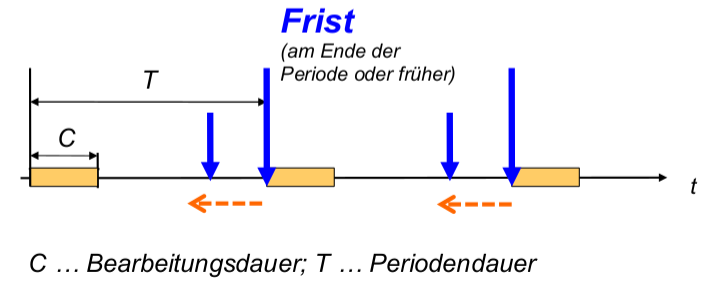
\includegraphics[width=\linewidth]{Assets/AdvancedOperatingSystems-echtzeit-periodisch-frist.png}
        \end{itemize*}
        \item[Modellierung] unendliche Folge identischer Aktivierungen: Instanzen, aktiviert mit konstanter Rate (Periode)
        %\item 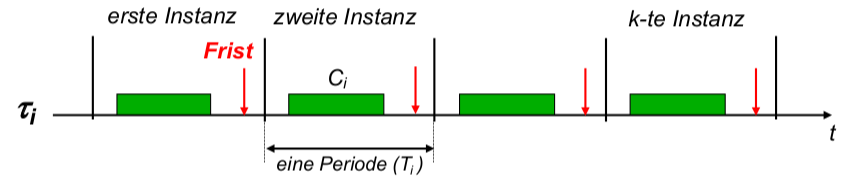
\includegraphics[width=\linewidth]{Assets/AdvancedOperatingSystems-echtzeit-periodisch-modellierung.png}
        \item[Aufgaben des Betriebssystems]
        \begin{itemize*}
            \item Wenn alle Spezifikationen eingehalten werden, muss Betriebssystem garantieren, dass
            \item zeitgesteuerte pP: mit ihrer spezifizierten Rate aktiviert werden und ihre Frist einhalten können
            \item ereignisgesteuerte pP: ihre Frist einhalten können
        \end{itemize*}
    \end{description*}

    \subsubsection{Aperiodische Prozesse (aP)}
    \begin{description*}
        \item typisch für unregelmäßig auftretende Ereignisse, z.B.:
        \begin{itemize*}
            \item Überfahren der Spurgrenzen, Unterschreiten des Sicherheitsabstands $\rightarrow$ Reaktion des Fahrassistenzsystems
            \item Nutzereingaben in Multimediasystemen ( $\rightarrow$ Spielkonsole)
        \end{itemize*}
        \item[Prozessaktivierung] ereignisgesteuert
        \item[Fristen] oft weich (aber anwendungsabhängig)
        \item[Aufgaben des Betriebssystems] unter Einhaltung der Prozessspezifikationen muss BS für Einhaltung der Fristen sorgen
        \item[Modellierung] bestehen ebenfalls aus (maximal unendlicher) Folge identischer Aktivierungen (Instanzen); aber: Aktivierungszeitpunkte nicht regelmäßig (möglich: nur genau eine Aktivierung)
        %\item 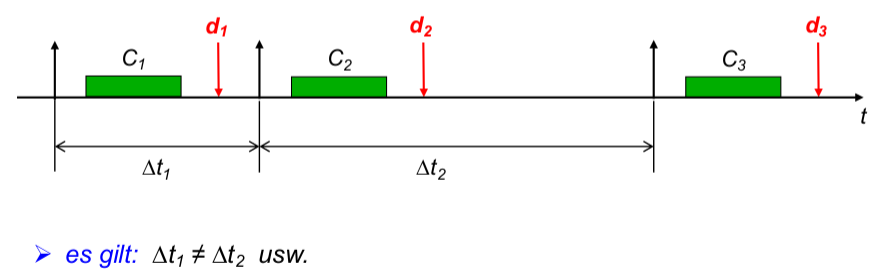
\includegraphics[width=\linewidth]{Assets/AdvancedOperatingSystems-echtzeit-aperiodisch-modellierung.png}
    \end{description*}

    \subsubsection{Parameter von Echtzeit-Prozessen}
    \begin{center}
        %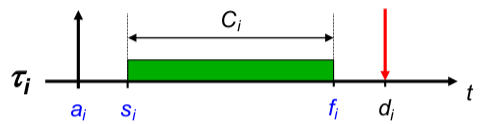
\includegraphics[width=.45\linewidth]{Assets/AdvancedOperatingSystems-echtzeit-parameter-instanz.png}
        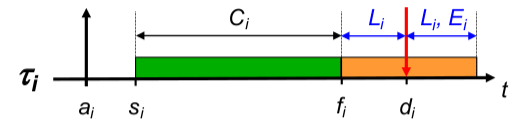
\includegraphics[width=.45\linewidth]{Assets/AdvancedOperatingSystems-echtzeit-parameter-instanz2.png}
        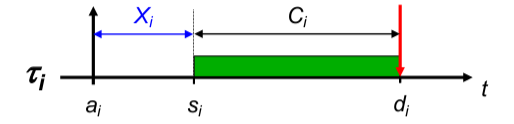
\includegraphics[width=.45\linewidth]{Assets/AdvancedOperatingSystems-echtzeit-parameter-instanz3.png}
    \end{center}
    \begin{description*}
        \item[Ankunftszeitpunkt $a_i$] Prozess wird ablauffähig
        \item[Startzeitpunkt $s_i$] Prozess beginnt mit Ausführung
        \item[Beendigungszeitpunkt $f_i$] Prozess beendet Ausführung
        \item[Frist (deadline) $d_i$] Prozess sollte Ausführung spätestens beenden
        \item[Bearbeitungszeit (computation time) $C_i$] Zeit die Prozessor zur Bearbeitung der Instanz benötigt (ohne Unterbrechungen)
        \item[Unpünktlichkeit (lateness)] $L_i= f_i - d_i$ Zeit um die Prozess früher/später als Frist beendet
        \item[Verspätung (exceeding time)] $E_i= max(0, L_i)$ Zeitbetrag, den ein Prozess noch nach seiner Frist aktiv ist
        \item[Spielraum (Laxity)] $X_i = d_i - a_i - C_i$ maximale Verzögerungszeit bis Frist beendet werden kann ($f_i=d_i$)
        \item[criticality] Konsequenzen einer Fristüberschreitung (hart/weich)
        \item[Wert $V_i$] Ausdruck relativer Wichtigkeit eines Prozesses
    \end{description*}

    \subsection{Echtzeitfähige Betriebssysteme}
    \begin{enumerate*}
        \item Algorithmen, die Rechnersysteme echtzeitfähig machen
        \begin{itemize*}
            \item grundlegende Algorithmen zum Echtzeitscheduling
            \item Besonderheiten der Interruptbehandlung
            \item Besonderheiten der Speicherverwaltung
        \end{itemize*}
        \item Probleme, die behandelt werden müssen
        \begin{itemize*}
            \item Prioritätsumkehr
            \item Überlast
            \item Kommunikation-und Synchronisationsprobleme
        \end{itemize*}
    \end{enumerate*}

    \subsubsection{Echtzeitscheduling}
    \begin{description*}
        \item[Scheduling] wichtigster Einflussfaktor auf Zeitverhalten des Gesamtsystems
        \item[Echtzeit-Scheduling] unter Berücksichtigung der Fristen
    \end{description*}
    Fundamentale/wichtigste Strategien
    \begin{enumerate*}
        \item Ratenmonotones Scheduling (RM)
        \item Earliest Deadline First (EDF)
    \end{enumerate*}

    Annahmen der Scheduling-Strategien
    \begin{enumerate*}
        \item Alle Instanzen eines periodischen Prozesses $t_i$ treten regelmäßig und mit konstanter Rate auf. Das Zeitintervall $T_i$ zwischen zwei aufeinanderfolgenden Aktivierungen heißt Periode des Prozesses
        \item Alle Instanzen eines periodischen Prozesses $t_i$ haben den gleichen Worst-Case-Rechenzeitbedarf $C_i$
        \item Alle Instanzen eines periodischen Prozesses $t_i$ haben die gleiche relative Frist $D_i$, welche gleich der Periodendauer $T_i$ ist
        \item Alle Prozessesind kausal unabhängig voneinander (d.h. keine Vorrang- und Betriebsmittel-Restriktionen)
        \item Kein Prozess kann sich selbst suspendieren, z.B. E/A-Op
        \item Alle Prozesse werden mit ihrer Aktivierung sofort rechenbereit
        \item Jeglicher Betriebssystem-Overhead wird vernachlässigt
    \end{enumerate*}
    5-7 sind weitere Annahmen des Scheduling Modells

    \paragraph{Ratenmonotones Scheduling (RM)}
    \begin{itemize*}
        %\item \includegraphics[width=\linewidth]{Assets/AdvancedOperatingSystems-echtzeit-scheduling-rm.png}
        \item Voraussetzung: nur periodische Prozesse/Threads
        \item Strategie RM
        \begin{itemize*}
            \item Prozess/Thread mit höchster Ankunftsrate bekommt höchste statische Priorität
            \item Kriterium: Wie oft pro Zeiteinheit wird Prozess bereit?
            \item Scheduling-Zeitpunkt: nur einmal zu Beginn bzw. wenn neuer periodischer Prozess auftritt
            \item präemptiv: keine Verdrängung gleicher Prioritäten
        \end{itemize*}
        \item Optimalität: Unter allen Verfahren mit festen Prioritäten optimaler Algorithmus%, so dass kein anderes Verfahren eine Prozessmenge einplanen kann, die nicht von RM geplant werden kann
        \item Prozessor-Auslastungsfaktor
        \begin{itemize*}
            \item Bei Menge von n Prozessen $U=\sum_{i=1}^n \frac{C_i}{T_i}$
            \item mit $\frac{C_i}{T_i}$ Anteil an Prozessorzeit für jeden Prozess $t_i$
            \item und Zeit $U$ zur Ausführung der gesamten Prozessmenge
        \end{itemize*}
        \item Prozessorlast: $U$ ist folglich Maß für die durch Prozessmenge verursachte Last am Prozessor $\rightarrow$ Auslastungsfaktor
        \item Planbarkeitsanalyse einer Prozessmenge
        \begin{itemize*}
            \item allgemein kann RM Prozessor nicht 100\% auslasten
            \item kleinste obere Grenze des Auslastungsfaktors $U_{lub}$
            \item lub: ,,least upper bound''
        \end{itemize*}
        \item Obere Auslastungsgrenze bei RM
        \begin{itemize*}
            \item nach Buttazzo bei n Prozessen: $U_{lub}=n(2^{\frac{1}{n}}-1)$
            \item für $n\rightarrow\infty$ konvergiert $U_{lub}$ zu $ln\ 2 \approx 0,6931...$
            \item Wert nicht überschritten $\rightarrow$ beliebige Prozessmengen
        \end{itemize*}
    \end{itemize*}

    \paragraph{Earliest Deadline First (EDF)}
    \begin{itemize*}
        %\item \includegraphics[width=\linewidth]{Assets/AdvancedOperatingSystems-echtzeit-scheduling-edf.png}
        \item Voraussetzung: kann periodische/aperiodische Prozesse planen
        \item Optimalität: EDF in Klasse der Schedulingverfahren mit dynamischen Prioritäten: optimaler Algorithmus
        \item Strategie EDF
        \begin{itemize*}
            \item Prozess mit frühester Frist höchste dynamische Priorität
            \item Scheduling-Zeitpunkt: Bereitwerden eines Prozesses
            \item präemptiv: keine Verdrängung gleicher Prioritäten
        \end{itemize*}
        \item Planbarkeitsanalyse
        \begin{itemize*}
            \item mit Regeln $1-7$ max. Prozessorauslastung: $U_{lub}= 1\rightarrow$ Auslastung bis 100\%
            \item Menge von n Tasks planbar: $U=\sum_{i=1}^n \frac{C_i}{T_i}\leq 1$
            \item[$\leftarrow$] $U\textgreater1$ übersteigt die verfügbare Prozessorzeit; folglich kann niemals eine Prozessmenge mit dieser Gesamtauslastung planbar sein
            \item[$\rightarrow$] Beweis durch Widerspruch. Annahme: $U\leq 1$ und die Prozessmenge ist nicht planbar. Dies führt zu einem Schedule mit Fristverletzung zu einem Zeitpunkt $t_2$
        \end{itemize*}
    \end{itemize*}

    \paragraph{Vergleich: EDF vs. RM}
    \begin{center}
        \includegraphics[width=.8\linewidth]{Assets/AdvancedOperatingSystems-echtzeit-edf-vs-rm.png}
    \end{center}
    \begin{itemize*}
        \item RM
        \begin{itemize*}
            \item Prozessorwechsel: 16
            \item im allgemeinen Fall nicht immer korrekte Schedules bei 100\% Auslastung
            \item statisch Implementiert: jeweils eine Warteschlange pro Priorität
            \item Einfügen und Entfernen von Tasks: $O(1)$
            %\item \includegraphics[width=\linewidth]{Assets/AdvancedOperatingSystems-echtzeit-scheduling-rm-statisch.png}
        \end{itemize*}
        \item EDF
        \begin{itemize*}
            \item Prozessorwechsel: 12
            %\item Ursache: dynamische Prioritätenvergabe führt dazu, dass Instanz II von $t_2$ die gleiche Priorität wie Instanz A von $t_1$ hat $\rightarrow$ keine unnötige Verdrängung
            \item erzeugt auch bei Prozessorauslastung bis 100\% (immer) korrekte Schedules
            \item dynamisch Implementiert: balancierter Binärbaum zur Sortierung nach Prioritäten
            \item Einfügen und Entfernen von Tasks: $O(log\ n)$
            %\item \includegraphics[width=\linewidth]{Assets/AdvancedOperatingSystems-echtzeit-scheduling-edf-dynamisch.png}
        \end{itemize*}
    \end{itemize*}

    Prozesstypen in Multimedia-Anwendungen
    \begin{enumerate*}
        \item Echte periodische Multimedia-Prozesse (weiche Fristen)
        \begin{enumerate*}
            \item pünktliche periodische Prozesse mit konstantem Prozessorzeitbedarf $C$ für jede Instanz (unkomprimierte Audio- und Videodaten)
            \item pünktliche periodische Prozesse mit unterschiedlichem $C$ einzelner Instanzen (komprimierte Audio- und Videodaten)
            \item unpünktliche periodische Prozesse: verspätet/verfrühte
        \end{enumerate*}
        \item Prozesse nebenläufiger Nicht-Multimedia-Anwendungen
        \begin{itemize*}
            \item interaktiv: keine Fristen , keine zu langen Antwortzeiten Ansatz, maximal tolerierbare Verzögerung
            \item Hintergrund: zeitunkritisch, keine Fristen, dürfen nicht verhungern
        \end{itemize*}
    \end{enumerate*}

    \subsubsection{RC Algorithmus}
    \begin{itemize*}
        \item Ziel: spezifikationstreue Prozesse nicht bestrafen durch Fristüberschreitung aufgrund abweichender Prozesse
        \item Idee
        \begin{itemize*}
            \item grundsätzlich: Scheduling nach frühester Frist aufsteigend
            \item[$\rightarrow$] für vollständig spezifikationstreue Prozessmenge wie EDF
            \item Frist einer Instanz wird dynamisch angepasst: basierend auf derjenigen Periode, in der sie eigentlich sein sollte% lt. Spezifikation der Prozessornutzung: $U_i=\frac{C_i}{T_i}$
            \item Bsp.: $U_i =\frac{20}{40}=\frac{1}{2}$ (spez. Aktivitätsrate $0,5$/Periode)
        \end{itemize*}
        \item Variablen
        \begin{itemize*}
            \item $a_i$: Ankunftszeit der zuletzt bereitgewordenen Instanz
            \item $t_i^{virt}$: virtuelle verbrauchte Zeit in aktueller Periode
            \item $c_i^{virt}$: verbrauchte Netto-Rechenzeit
            \item $d_i$: dynamische Frist von $t_i$ für Priorität (EDF)
        \end{itemize*}
        \item Strategie
        \begin{itemize*}
            \item für eine bereite (lauffähige) Instanz von $t_i$: adaptiere dynamisch $d_i$ basierend auf $t_i^{virt}$
            \item für eine bereit gewordene Instanz von $t_i$: aktualisiere $t_i^{virt}$ auf akt. Systemzeit $(t)\rightarrow$ etwaiger ,,Zeitkredit'' verfällt
        \end{itemize*}
        \item Zeitpunkte, zu denen der Scheduler aktiv wird
        \begin{itemize*}
            \item aktuell laufender Prozess $t_i$ blockiert:  $RC(t_i)$
            \item Prozesse $t_i..._j$ werden bereit:  $for\ x\in[i,j]: RC(t_x)$
            \item periodischer ,,clock tick'' (Scheduling Interrupt) $RC(t_i)$
        \end{itemize*}
    \end{itemize*}

    %\paragraph{RC Algorithmus: Berechnung von $t_i^{virt}$}
    %Beispiel: Situation bei $t=20ms$
    %\includegraphics[width=\linewidth]{Assets/AdvancedOperatingSystems-rc-ti-berechnen-1.png}
    %Da $t_B$ aber noch weiteren Rechenbedarf hat: Situation bei $t=30ms$
    %\includegraphics[width=\linewidth]{Assets/AdvancedOperatingSystems-rc-ti-berechnen-2.png}

    %\paragraph{RC Algorithmus: Adaptionsfunktion}
    %Für Prozess ti zu jedem Scheduling-Zeitpunkt:
    %\begin{Shaded}
    %\begin{Highlighting}[]
    %\NormalTok{RC (t_i) \{}
    % \ControlFlowTok{if}\NormalTok{ (t_i. status wurde auf BEREIT gesetzt) \{}
    %\NormalTok{ t_i^virt := max( t_i^virt , t ); }\CommentTok{//kein Zeitkredit {-}\textgreater{} kein ,,Nachholen\textquotesingle{}\textquotesingle{} von verpassten/ungenutzten Perioden}
    %\NormalTok{ \} }\ControlFlowTok{else}\NormalTok{ \{}
    %\NormalTok{ c_i^virt := Gesamtprozessorzeit seit letztem Aufruf RC(t_i);}
    %\NormalTok{ t_i^virt := t_i^virt + c_i^virt / U_i ; }\CommentTok{//Zeitwert, bis zu dem t_i Rechenzeit gemäß seiner Rate U_i erhalten hat}
    %\NormalTok{ \}}
    % \ControlFlowTok{if}\NormalTok{ (t_i. status != BLOCKIERT) \{}
    %\NormalTok{ finde k, so dass gilt:}
    %\NormalTok{ a_i + (k {-} }\DecValTok{1}\NormalTok{) * T_i \textless{}= t_i^virt \textless{} a_i + k * T_i ; }\CommentTok{// finde diejenige (aktuelle oder zukünftige) Periode, in der t_i^virt liegt}
    %\NormalTok{ d_i := a_i + k * T_i ; }\CommentTok{// setze d_i auf deren Periodenende}
    %\NormalTok{ \}}
    %\NormalTok{\}}
    %\end{Highlighting}
    %\end{Shaded}


    %anschließendes Scheduling (präemptiv) = EDF
    %\begin{Shaded}
    %\begin{Highlighting}[]
    %\NormalTok{SCHED := \{t_i |t_i.status == BEREIT ⋀ d_i minimal \}; }\CommentTok{// bereite(r) Prozess(e) mit nächster Frist}
    %\ControlFlowTok{if}\NormalTok{ (∃ t_j : t_j.status == LAUFEND) ⋀ ( d_j ≤ d_i )}
    % \ControlFlowTok{do}\NormalTok{ nothing; }\CommentTok{// ggf. laufenden Prozess bevorzugen}
    %\ControlFlowTok{else}
    %\NormalTok{ preempt(rnd_member( SCHED )); }\CommentTok{// sonst: irgendein Prozess mit nächster Frist verdrängt den laufenden}
    %\end{Highlighting}
    %\end{Shaded}


    \paragraph{Umgang mit abweichenden Prozessen unter RC}
    %\includegraphics[width=\linewidth]{Assets/AdvancedOperatingSystems-rc-abweichende-prozesse.png}
    %Prozesse, die sich entsprechend ihrer Spezifikation verhalten, erhalten bis zum Ende jeder spezifizierten Periode ihren spezifizierten Anteil an Prozessorzeit.

    Auswirkung auf verschiedene Prozesstypen
    \begin{description*}
        \item[pünktlich] Einhaltung der Frist in jeder Periode garantiert
        \item[verspätet] nur aktuelle Periode betrachtet, Nachholen ,,ausgelassener Perioden'' nicht möglich
        \item[gierig] Prozessorentzug, sobald andere lauffähige Prozesse frühere Fristen aufweisen
        \item[nicht-periodische Hintergrundprozesse] pro ,,Periode'' wird spezifizierte Prozessorrate garantiert
    \end{description*}

    \subsubsection{Umgang mit gemischten Prozessmengen}
    %Hintergrund-Scheduling
    \begin{center}
        \includegraphics[width=.5\linewidth]{Assets/AdvancedOperatingSystems-gemischte-prozessmenge.png}
    \end{center}
    \begin{itemize*}
        \item rechenbereite Prozesse auf 2 Warteschlangen aufgeteilt (einfache Variante eines Mehr-Ebenen-Scheduling )
        \item Warteschlange 1
        \begin{itemize*}
            \item alle periodischen Prozesse
            \item mit höchster Priorität mittels RM oder EDF bedient
        \end{itemize*}
        \item Warteschlange 2
        \begin{itemize*}
            \item alle aperiodischen Prozesse
            \item nur bedient, wenn keine wartenden Prozesse in W1
        \end{itemize*}
    \end{itemize*}


    \paragraph{Hintergrund-Scheduling: Vor- und Nachteile}
    \begin{itemize*}
        \item Hauptvorteil einfache Implementierung
        \item Nachteile
        \begin{itemize*}
            \item Antwortzeit \textbf{aperiodischer Prozesse} kann zu lang werden
            \item[$\rightarrow$] Verhungern möglich
            \item nur für relativ zeitunkritische aperiodische Prozesse
        \end{itemize*}
        %\item Beispiel: Hintergrund-Scheduling mit RM
        %\item \includegraphics[width=\linewidth]{Assets/AdvancedOperatingSystems-hintergrund-scheduling.png}
    \end{itemize*}

    \paragraph{Optimierung: Server-Prozess}
    \begin{itemize*}
        \item Prinzip: periodisch aktivierter Prozess benutzt zur Ausführung aperiodischer Prozessoranforderungen
        \item Beschreibung Server-Prozess: durch Parameter äquivalent zu wirklichem periodischen Prozess
        \item Arbeitsweise Server-Prozess folgend
        \item geplant mit gleichem S-Algorithmus wie periodische Prozesse
        \item zum Aktivierungszeitpunkt vorliegende aperiodische Anforderungen bedient bis zur Kapazität des Servers
        \item keine aperiodischen Anforderungen: Server suspendiert sich bis Beginn der nächsten Periode %(Schedule wird ohne ihn weitergeführt $\rightarrow$ Prozessorzeit für periodische Prozesse)
        \item Kapazität in jeder Server-Periode neu ''aufgeladen''
    \end{itemize*}
    %Beispiel: Server-Prozess mit RM
    %\includegraphics[width=\linewidth]{Assets/AdvancedOperatingSystems-rm-server-prozess.png}

    \paragraph{Optimierung: Slack-Stealing}
    \begin{itemize*}
        \item Prinzip: passiver Prozess ,,slack stealer'' (kein periodischer Server)
        \item so viel Zeit wie möglich für aperiodische Anforderungen sammeln
        \item realisiert durch ,,slackstealing'' bei periodischen Prozessen
        \item letztere auf Zeit-Achse so weit nach hinten geschoben, dass Frist und Beendigungszeitpunkt zusammenfallen
        \item Sinnvoll, da Beenden vor Frist keine Vorteile bringt
        \item[$\rightarrow$] Verbesserung der Antwortzeiten für aperiodische Anforderungen
        %\item \includegraphics[width=\linewidth]{Assets/AdvancedOperatingSystems-slack-stealing.png}
    \end{itemize*}

    \subsubsection{Prioritätsumkehr}
    Mechanismen zur Synchronisation und Koordination sind häufige Ursachen für kausale Abhängigkeiten zwischen Prozessen
    \begin{itemize*}
        \item \emph{kritischer Abschnitt}: Sperrmechanismen stellen wechselseitigen Ausschluss durch nebenläufige Prozesse sicher
        \item Benutzung von exklusiven, nichtentziehbaren Betriebsmitteln
        \item[$\rightarrow$] Wenn ein Prozess einen kritischen Abschnitt betreten hat, darf er aus diesem nicht verdrängt werden %(durch anderen Prozess, der dasselbe Betriebsmittel nutzen will)
        \item Konflikt: kritische Abschnitte vs. Echtzeit-Prioritäten
        \item Prozess mit höherer Priorität ablauffähig $\rightarrow$ muss abwarten bis niederpriorisierter Prozess kritischen Abschnitt verlässt
        \item (zeitweise) Prioritätsumkehr möglich% d.h. aus einer (Teil-) Menge von Prozessen muss derjenige mit höchster Priorität auf solche mit niedrigerer Priorität warten
    \end{itemize*}

    Ursache der Prioritätsumkehr
    \begin{itemize*}
        \item \includegraphics[width=.7\linewidth]{Assets/AdvancedOperatingSystems-prioritätsumkehr-ursache.png}
        \item Prioritätsumkehr bei Blockierung an nichtentziehbarem, exklusivem Betriebsmittel
        \item $\rightarrow$ unvermeidlich
    \end{itemize*}

    Folgen der Prioritätsumkehr
    \begin{itemize*}
        \item Kritisch bei zusätzlichen Prozessen mittlerer Priorität
        \item \includegraphics[width=.5\linewidth]{Assets/AdvancedOperatingSystems-prioritätsumkehr-folgen.png}
        \item Lösung: Priority Inheritance Protocol (PIP)
    \end{itemize*}

    \subsubsection{Überlast}
    \begin{itemize*}
        \item Definition: kritische Situation, bei der benötigte Menge an Prozessorzeit die Kapazität des vorhandenen Prozessors übersteigt %$(U< 1)$
        \item[$\rightarrow$] nicht alle Prozesse können Fristen einhalten
        \item Hauptrisiko: kritische Prozesse können Fristen nicht einhalten $\rightarrow$ Gefährdung funktionaler und anderer nichtfkt. Eigenschaften ( $\rightarrow$ harte Fristen!)
        \item Stichwort: ,,graceful degradation'' statt unkontrollierbarer Situation $\rightarrow$ Wahrung von Determinismus
    \end{itemize*}

    Wichtigkeit eines Prozesses
    \begin{itemize*}
        %\item Minimallösung (lebenswichtig für Echtzeit-System)
        \item Unterscheidung zwischen Zeitbeschränkungen (Fristen) und tatsächlicher Wichtigkeit eines Prozesses für System
        \item Wichtigkeit eines Prozesses ist unabhängig von seiner Periodendauer und irgendwelchen Fristen
        \item z.B. kann Prozess trotz späterer Frist wichtiger als anderer mit früherer Frist sein
        %\item Beispiel: Bei chemischem Prozess könnte Temperaturauswertung jede 10s wichtiger sein als Aktualisierung graphischer Darstellung an Nutzerkonsole jeweils nach 5s
    \end{itemize*}

    Umgang mit Überlast: alltägliche Analogien
    \begin{enumerate*}
        \item Weglassen weniger wichtiger Aktionen (kein Frühstück...)
        \item Verkürzen von Aktivitäten (Katzenwäsche...)
        \item Kombinieren (kein Frühstück + Katzenwäsche + ungekämmt)
    \end{enumerate*}

    Wichtung von Prozessen
    \begin{itemize*}
        \item Parameter V für jeden Prozess/Thread einer Anwendung
        \item spezifiziert relative Wichtigkeit eines Prozesses/Thread im Verhältnis zu anderen der gleichen Anwendung
        \item bei Scheduling: V stellt zusätzliche Randbedingung (primär: Priorität aufgrund von Frist, sekundär: Wichtigkeit)
    \end{itemize*}

    Obligatorischer und optionaler Prozessanteil
    \begin{itemize*}
        \item Aufteilung der Gesamtberechnung eines Prozesses in zwei Phasen
        \item Möglichkeit der Nutzung des anpassbaren Prozessorzeitbedarfs
        \item Bearbeitungszeitbedarf eines Prozesses zerlegt in
        \begin{enumerate*}
            \item obligatorischer Teil: unbedingt und immer ausführen $\rightarrow$ liefert bedingt akzeptables Ergebnis
            \item optionaler Teil: nur bei ausreichender Lapazität ausführen $\rightarrow$ verbessert erzieltes Ergebnis
        \end{enumerate*}
        \item Prinzip in unterschiedlicher Weise verfeinerbar
        %\item \includegraphics[width=\linewidth]{Assets/AdvancedOperatingSystems-obligatorisch-optionaler-prozessanteil.png}
    \end{itemize*}

    \subsubsection{Echtzeit-Interruptbehandlung}
    \begin{itemize*}
        \item Fristüberschreitung durch ungeeignete Interruptbearbeitung
        %\item \includegraphics[width=\linewidth]{Assets/AdvancedOperatingSystems-interruptbehandlung-fristüberschreitung.png}
        \item Interrupt wird nur registriert (deterministischer Zeitaufwand)
        \item tatsächliche Bearbeitung der Interruptroutine muss durch Scheduler eingeplant werden $\rightarrow$ Pop-up Thread
        %\item \includegraphics[width=\linewidth]{Assets/AdvancedOperatingSystems-interruptbehandlung-lösung.png}
    \end{itemize*}

    \subsection{Echtzeit-Speicherverwaltung}
    \begin{itemize*}
        \item Hauptanliegen: Fristen einhalten
        \item unkontrollierbare Verzögerungen der Prozessbearbeitung vermeiden
        \item Ressourcenzuordnung, deswegen:
        \begin{enumerate*}
            \item keine Ressourcen-Zuordnung ,,on-demand'' sondern ,,Pre-Allokation'' (=Vorab)
            \item keine dynamische Ressourcenzuordnung, sondern Zuordnung maximal benötigter Menge bei Pre-Allokation
        \end{enumerate*}
    \end{itemize*}

    \paragraph{Hauptspeicherverwaltung}
    \begin{itemize*}
        \item bei Anwendung existierender Paging-Systeme
        \item durch unkontrolliertes Ein-/Auslagern ,,zeitkritischer'' Seiten (-inhalte): unkontrollierbare Zeitverzögerungen möglich
        \item Technik: ,,Festnageln'' von Seiten im Speicher (Memory Locking)
    \end{itemize*}

    \paragraph{Sekundärspeicherverwaltung}
    \begin{itemize*}
        \item Primärziel: Wahrung der Echtzeitgarantien
        \begin{itemize*}
            \item naheliegend: EA-Scheduling nach Fristen $\rightarrow$ EDF
            \item für Zugriffsreihenfolge auf Datenblöcke: lediglich deren Fristen maßgebend (weitere Regeln existieren nicht)
        \end{itemize*}
        \item Resultat bei HDDs
        \begin{itemize*}
            \item ineffiziente Bewegungen der Lese-/Schreibköpfe
            \item nichtdeterministische Positionierzeiten
            \item geringer Durchsatz
        \end{itemize*}
        \item Fazit: Echtzeit-Festplattenscheduling $\rightarrow$ Kompromiss zwischen Zeitbeschränkungen und Effizienz
        \item bekannte Lösungen: Modifikation/Kombination von EDF
    \end{itemize*}
    $\rightarrow$ realisierte Strategien:
    \begin{enumerate*}
        \item SCAN-EDF (Kopfbewegung in eine Richtung bis Mitte-/Randzylinder; EDF über alle angefragten Blöcke in dieser
        Richtung)
        \item Group Sweeping (SCAN nach Fristen gruppenweiser Bedienung)
        \item Mischstrategien
    \end{enumerate*}
    \begin{itemize*}
        \item Vereinfachung: o.g. Algorithmen i.d.R. zylinderorientiert
        \item[$\rightarrow$] berücksichtigen bei Optimierung nur Positionierzeiten (Positionierzeit meist $>>$ Latenzzeit)
    \end{itemize*}
    \begin{center}
        \includegraphics[width=.5\linewidth]{Assets/AdvancedOperatingSystems-sekundärspeicherverwaltung-festplatte.png}
    \end{center}

    \subsection{Kommunikation und Synchronisation}
    \begin{itemize*}
        \item zeitlichen Nichtdeterminismus vermeiden: Interprozess-Kommunikation
        \begin{itemize*}
            \item Minimierung blockierender Kommunikationsoperationen
            \item indirekte Kommunikation $\rightarrow$ Geschwindigkeitsausgleich
            \item keine FIFO-Ordnungen (nach Fristen priorisieren)
        \end{itemize*}
        \item Synchronisation: keine FIFO-Ordnungen
    \end{itemize*}

    \paragraph{Cyclic Asynchronous Buffer (CAB)}
    \begin{center}
        \includegraphics[width=.5\linewidth]{Assets/AdvancedOperatingSystems-kommunikation-cab.png}

        Kommunikation zwischen 1 Sender und n Empfängern
    \end{center}
    \begin{itemize*}
        \item nach erstem Schreibzugriff: garantiert niemals undefinierte Wartezeiten durch Blockierung von Sender/Empfänger
        \item Lesen/Überschreiben in zyklischer Reihenfolge:
        %\item \includegraphics[width=\linewidth]{Assets/AdvancedOperatingSystems-kommunikation-zyklisch-cab.png}
        \item Most-Recently-Written (MRW) Zeiger auf jüngstes, durch Sender vollständig geschriebenes Element
        \item Least-Recently-Written (LRW) Zeiger auf ältestes durch Sender geschriebenes Element
        \item sowohl \emph{MRW} als auch \emph{LRW} können ausschließlich durch Sender manipuliert werden $\rightarrow$ keine inkonsistenten Zeiger durch konkurrierende Schreibzugriffe
        \item sowohl \emph{MRW} als auch \emph{LRW} zeigen niemals auf ein Element, das gerade geschrieben wird $\rightarrow$ keine inkonsistenten Inhalte durch konkurrierende Schreib-/Lesezugriffe
        \item Regeln für Sender
        \begin{itemize*}
            \item muss \textbf{nach} jedem Schreiben \emph{MRW} auf geschriebenes Element setzen
            \item muss \textbf{bevor} \emph{LRW} geschrieben wird \emph{LRW} inkrementieren
        \end{itemize*}
        \item Regel für Empfänger: muss immer nach Lesen von \emph{MRW} als nächstes \emph{LRW} anstelle des Listennachbarn lesen
        %\item Sender-Regeln: \includegraphics[width=\linewidth]{Assets/AdvancedOperatingSystems-cab-sender-regel.png}
        %\item Empfänger-Regel: \includegraphics[width=\linewidth]{Assets/AdvancedOperatingSystems-cab-empfänger.png}
    \end{itemize*}

    Sonderfall 1: Empfänger schneller als Sender
    \begin{itemize*}
        \item nach Zugriff auf MRW muss auf Lesesequenz bei LRW fortgesetzt werden $\rightarrow$ transparenter Umgang mit nicht-vollem Puffer
        \item Abschwächung der Ordnungsgarantien:Empfänger weiß nur, dass Aktualität der Daten zwischen LRW und MRW liegt
        \item Empfänger niemals durch leeren Puffer blockiert
        %\item \includegraphics[width=\linewidth]{Assets/AdvancedOperatingSystems-cab-sonderfall-1.png}
    \end{itemize*}

    Sonderfall 2: Sender schneller als Empfänger
    \begin{itemize*}
        \item Schreiben in Puffer in Reihenfolge der Elemente $\rightarrow$ keine blockierenden Puffergrenzen $\rightarrow$ niemals Blockierung des Senders
        \item keine Vollständigkeitsgarantien: Empfänger kann nicht sicher sein, eine temporal stetige Sequenz zu lesen
        \item[$\rightarrow$] Szenarien, in denen Empfänger sowieso nur an aktuellsten Daten interessiert (z.B. Sensorwerte)
        %\item \includegraphics[width=\linewidth]{Assets/AdvancedOperatingSystems-cab-sonderfall-2.png}
    \end{itemize*}

    Konkurrierende Zugriffe
    \begin{itemize*}
        \item ... sind durch Empfänger immer unschädlich (da lesend)
        \item ... müssen vom Sender nach Inkrementieren von LRW nicht-blockierend erkannt werden (Semaphormodell ungeeignet)
        \item schnellerer Sender überspringtein gesperrtes Element durch erneutes Inkrementieren von LRW, MRW muss nachziehen
        %\item \includegraphics[width=\linewidth]{Assets/AdvancedOperatingSystems-cab-konkurrierende-zugriffe.png}
    \end{itemize*}

    \subsection{Architekturen}
    \begin{itemize*}
        \item müssen Echtzeitmechanismen unterstützen; ermöglicht entsprechende Strategien zur Entwicklungs-oder Laufzeit
        \item müssen funktional geringe Komplexität aufweisen $\rightarrow$ theoretische und praktische Beherrschung von Nichtdeterminismus
        \item Architekturen für komplementäre NFE
        \begin{itemize*}
            \item Sparsamkeit $\rightarrow$ hardwarespezifische Kernelimplementierung
            \item Adaptivität $\rightarrow$ $\mu$Kernel, Exokernel
        \end{itemize*}
        \item zu vermeiden
        \begin{itemize*}
            \item starke HW-Abstraktion $\rightarrow$ Virtualisierungsarchitekturen
            \item Kommunikation und Synchronisationskosten $\rightarrow$ verteilte BS
            \item Hardwareunabhängigkeit und Portabilität $\rightarrow$ vgl. Mach
        \end{itemize*}
    \end{itemize*}

    \subsection{Beispiel-Betriebssysteme}

    VRTX (Versatile Real-Time Executive)
    \begin{itemize*}
        \item Entwickler: Hunter \& Ready
        \item Eckdaten: Makrokernel
        \item war erstes kommerzielles Echtzeitbetriebssystem für eingebettete Systeme
        \item Nachfolger (1993 bis heute): Nucleus RTOS (Siemens)
        \item Anwendung: Eingebettete Systeme in Automobilen, Mobiltelefone
        \item Einsatzgebiete im Hubble-Weltraumteleskop
    \end{itemize*}

    VxWorks
    \begin{itemize*}
        \item Entwickler: Wind River Systems (USA)
        \item Eckdaten: modularer Makrokernel
        \item Erfolgsfaktor: POSIX-konforme API
        \item ähnlich QNX: ,,skalierbarer'' Kernel, zuschneidbar auf Anwendungsdomäne ($\rightarrow$ Adaptivitätsansatz)
        \item Anwendung: eingebettete Systeme, Luft-und Raumfahrt, Unterhaltungselektronik
        \item Einsatzgebiete: NASA Mars Rover, SpaceX Dragon
    \end{itemize*}

    DRYOS
    \begin{itemize*}
        \item Entwickler: Canon Inc.
        \item Eckdaten: Mikrokernel(Größe: 16 kB)
        \item Echtzeit-Middleware (Gerätetreiber $\rightarrow$ Objektive)
        \item Anwendungen: AE-und AF-Steuerung/-Automatik, GUI, Bildbearbeitung, RAW-Konverter, ...
        \item POSIX-kompatible Prozessverwaltung
        %\item \includegraphics[width=\linewidth]{Assets/AdvancedOperatingSystems-dryos.png}
    \end{itemize*}

    DROPS (Dresden Real-Time Operating System)
    \begin{itemize*}
        \item Entwickler: TU Dresden, Lehrstuhl Betriebssysteme
        \item Eckdaten: Multi-Server-Architektur auf Basis eines L4-Mikrokerns
        %\item \includegraphics[width=\linewidth]{Assets/AdvancedOperatingSystems-drops.png}
    \end{itemize*}

    \section{Adaptivität (Flexibility)}
    \begin{itemize*}
        \item als unmittelbar geforderte NFE: eingebettete Systeme, Systeme in garstiger Umwelt
        \item diese Anwendungsdomänen fordern typischerweise auch andere wesentliche NFE
        \item[$\rightarrow$] Adaptivität als komplementäre NFE zur Förderung von
    \end{itemize*}
    \begin{description*}
        \item[Robustheit] funktionale Adaptivitätdes BS reduziert Kernelkomplexität %($\rightarrow$ kleiner, nicht adaptiver $\mu$Kernel)
        \item[Sicherheit] TCB-Größe $\rightarrow$ Verifizierbarkeit, adaptive Reaktion auf Bedrohungen
        \item[Echtzeitfähigkeit] adaptives Scheduling/Überlast/Interruptbehandlung
        \item[Performanz] Last-und Hardwareadaptivität
        \item[Erweiterbarkeit] von Abstraktionen, Schnittstellen, Multiplexing
        \item[Wartbarkeit] Anpassung des BS an Anwendungen, nicht umgekehrt
        \item[Sparsamkeit] Lastadaptivität, adaptive Datenstrukturen
    \end{description*}
    \begin{itemize*}
        \item Begriff
        \begin{itemize*}
            \item Fähigkeit eines Systems, sich an breites Spektrum verschiedener Anforderungen anzupassen
            \item[=] so gebaut, dass breites Spektrum verschiedener nicht funktionaler Eigenschaften unterstützt
            \item letztere: komplementär zur allgemeinen NFE Adaptivität
        \end{itemize*}
        \item Adaptivität jeweils anhand komplementärer Eigenschaften dargestellt:
        \begin{itemize*}
            \item Exokernel: \{Adaptivität\}$\cup$\{Performanz, Echtzeitfähigkeit,Wartbarkeit, Sparsamkeit\}
            \item Virtualisierung: \{Adaptivität\}$\cup$\{Wartbarkeit, Sicherheit, Robustheit\}
            \item Container: \{Adaptivität\}$\cup$\{Wartbarkeit, Portabilität, Sparsamkeit\}
        \end{itemize*}
        \item Beispielsysteme
        \begin{itemize*}
            \item Exokernel OS: Aegis/ExOS, Nemesis, MirageOS
            \item Virtualisierung: Vmware, VirtualBox, Xen
            \item Containersoftware: Docker
        \end{itemize*}
    \end{itemize*}

    \subsection{Exokernelarchitektur}
    \begin{itemize*}
        \item Grundfunktion von Betriebssystemen
        \begin{itemize*}
            \item physische Hardware darstellen als abstrahierte Hardware mit komfortableren Schnittstellen
            %\item \includegraphics[width=\linewidth]{Assets/AdvancedOperatingSystems-exokernelarchitekturen.png}
            \item Schnittstelle zu Anwendungen (API): Abstraktionen der Hardware
        \end{itemize*}
        \item Problem: Implementierungsspielraumfür Anwendungen wird begrenzt
        \begin{enumerate*}
            \item Vorteile domänenspezifischer Optimierungender Hardwarebenutzung können nicht ausgeschöpft werden $\rightarrow$ \textbf{Performanz, Sparsamkeit}
            \item die Implementierung existierender Abstraktionen kann bei veränderten Anforderungen nicht an Anwendungen angepasst werden $\rightarrow$ \textbf{Wartbarkeit}
            \item Hardwarespezifikationen, insbesondere des Zeitverhaltens (E/A, Netzwerk etc.), werden von Effekten des BS-Management überlagert $\rightarrow$ \textbf{Echtzeitfähigkeit}
        \end{enumerate*}
    \end{itemize*}


    \subsubsection{Exokernelmechanismen}
    \begin{center}
        \includegraphics[width=.6\linewidth]{Assets/AdvancedOperatingSystems-exokernel-architektur.png}
        %\includegraphics[width=\linewidth]{Assets/AdvancedOperatingSystems-exokernel-beispiel.png}
    \end{center}
    \begin{itemize*}
        \item Trennung von Schutz und Abstraktion der Ressourcen
        \item Ressourcen-Schutz und -Multiplexing verbleibt beim Kernel
        \item Ressourcen-Abstraktion Aufgabe der Library-Betriebssysteme
        \item[$\rightarrow$] autonome Management-Strategien durch in Anwendungen importierte Funktionalität
        \begin{enumerate*}
            \item systemweit(durch jeweiliges BS vorgegebene) starre Hardware-Abstraktionen vermieden
            \item anwendungsdomänenspezifische Abstraktionen sehr einfach
            \item (Wieder-) Verwendung eigener/fremder Managementfunktionalität wesentlich erleichtert $\rightarrow$ komplementäre NFEn (Performanz, Sparsamkeit, ...)
        \end{enumerate*}
        \item Funktion des Exokernels
        \begin{itemize*}
            \item Prinzip: definiert Low-level-Schnittstelle (so hardwarenah wie möglich)
            \item[$\rightarrow$] Adressierung ermöglichen ohne Informationen über Seiten, Segmente, Paging-Attribute, ...
            \item Library-Betriebssysteme: implementieren darauf jeweils geeignete anwendungsnahe Abstraktionen
            \item Anwendungsprogrammierer: wählen geeignete Library-Betriebssysteme bzw. schreiben ihre eigenen Exokernelmechanismen
        \end{itemize*}
        \item prinzipielle Exokernelmechanismen am Beispiel Aegis/ExOS
        \begin{description*}
            \item[implementiert] Multiplexing der Hardware-Ressourcen
            \item[exportiert] geschützte Hardware-Ressourcen
        \end{description*}
        \item minimal: drei Arten von Mechanismen
    \end{itemize*}
    \begin{description*}
        \item[Secure Binding] erlaubt geschützte Verwendung von Hardware- Ressourcen durch Anwendungen, Behandlung von Ereignissen
        \item[Visible Resource Revocation] beteiligt Anwendungen am Entzug von Ressourcen mittels (kooperativen) Ressourcen-Entzugsprotokolls
        \item[Abort-Protokoll] erlaubt ExokernelBeendigung von Ressourcenzuordnungen bei unkooperativen Applikationen
    \end{description*}


    \subsubsection{Secure Binding}
    \begin{itemize*}
        \item Schutzmechanismus, trennt Autorisierung zur Benutzung einer Ressource von tatsächlicher Benutzung
        \item implementiert für Exokernel erforderliches Zuordnungswissen von (HW-)Ressource zu Mangement-Code
        \item $\rightarrow$ ''Binding'' in Aegis implementiert als Unix-Hardlink auf Metadatenstruktur zu einem Gerät im Kernelspeicher
        \item Zur Implementierung benötigt
        \begin{itemize*}
            \item Hardware-Unterstützung zur effizienten Rechteprüfung (HW-Caching)
            \item Software-Caching von Autorisierungsentscheidungen im Kernel
            \item Downloading von Applikationscode in Kernel zur effizienten Durchsetzung
        \end{itemize*}
        \item ,,Secure Binding'' erlaubt Exokernel Schutz von Ressourcen ohne deren Semantik verstehen zu müssen
    \end{itemize*}

    \subsubsection{Visible Resource Revocation}
    monolithische BS: entziehen Ressourcen ,,unsichtbar'', d.h. transparent für Anwendungen
    \begin{itemize*}
        \item Vorteil: im allgemeinen geringere Latenzzeiten, einfacheres und komfortableres Programmiermodell
        \item Nachteil: Anwendungen erhalten keine Kenntnis über Entzug
        \item[$\rightarrow$] erforderliches Wissen für Management-Strategien
    \end{itemize*}
    Exokernel-BS: entziehen Ressourcen ,,sichtbar'' $\rightarrow$ Dialog zwischen Exokernel und Library-BS
    \begin{itemize*}
        \item Vorteil: effizientes Management durch Library-BS möglich %(z.B. Prozessor: nur tatsächlich benötigte Register werden bei Entzug gespeichert)
        \item Nachteil: Performanz bei sehr häufigem Entzug, Verwaltungs-und Fehlerbehandlungsstrategien zwischen verschiedenen Library-BS müssen korrekt und untereinander kompatibel sein...
        \item[$\rightarrow$] Abort-Protokoll notwendig, falls dies nicht gegeben ist
    \end{itemize*}

    \subsubsection{Abort-Protokoll}
    \begin{itemize*}
        \item Ressourcenentzug bei unkooperativen Library-Betriebssystemen
        \item notwendig aufgrund von Visible Ressource Revocation
        \item Dialog:
        \begin{itemize*}
            \item Exokernel: ,,Bitte Seitenrahmen x freigeben.''
            \item Library-BS: ,,...''
            \item Exokernel: ,,Seitenrahmen x innerhalb von 50 $\mu$s freigeben''
            \item Library-BS: ,,...''
            \item Exokernel: (führt Abort-Protokoll aus)
            \item Library-BS: X (,,Abort'' hier Prozess terminieren)
        \end{itemize*}
        \item harte Echtzeit-Fristen in wenigsten Anwendungen berücksichtigt
        \item[$\rightarrow$] Abort = nur Widerruf der Secure Bindings, nicht Terminierung% der jeweiligen Ressource für die unkooperative Anwendung, nicht deren Terminierung (= unsichtbarer Ressourcenentzug) 
        \item[$\rightarrow$] anschließend: Informieren des entsprechenden Library-BS
        \item ermöglicht sinnvolle Reaktion des Library-BS %(in Library-BS wird ,,Repossession''-Exception ausgelöst, so dass auf Entzug geeignet reagiert werden kann)
        \item bei zustandsbehafteten Ressourcen: Exokernel kann Zustand auf Hintergrundspeicher sichern $\rightarrow$ Management-Informationen zum Aufräumen durch Library-BS
    \end{itemize*}

    \subsubsection{Aegis mit Library-OS ExOS}
    \begin{itemize*}
        \item sehr effiziente Exokerne, begrenzte Anzahl einfacher Systemaufrufe (~10) und Kernel-interne Primitiven
        \item sicheres Hardware-Multiplexing auf niedriger Abstraktionsebene (,,low-level'') mit geringem Overhead
        \item trad. Abstraktionen (VMM, IPC) auf Anwendungsebene effizient implementierbar $\rightarrow$ einfache Erweiter-/Spezialisierbarkeit %bzw. Ersetzbarkeit dieser Abstraktionen
        \item hochspezialisierte Implementierungen von Abstraktionen generierbar%, die genau auf Funktionalität und Performanz-Anforderungen dieser Anwendung zugeschnitten
        \item geschützte Kontrollflussübergabe: als IPC-Primitive im Aegis-Kernel, 7-mal schneller als zuvor %damals beste Implementierung
        \item Ausnahmebehandlung bei Aegis: 5-mal schneller als bei damals bester Implementierung
        \item durch Aegis: Flexibilität von ExOS, mit Mikrokernel nicht erreichbar
        \item Aegis erlaubt Anwendungen Konstruktion effizienter IPC-Primitiven ($\Delta \mu$Kernel: nicht vertrauenswürdige Anwendungen können keinerlei spezialisierte IPC-Primitiven nutzen)
    \end{itemize*}

    \subsubsection{Xok mit Library-OS ExOS}
    \begin{itemize*}
        \item für x86-Hardware implementiert
        \item Kernel-Aufgaben: Multiplexing von Festplatte, Speicher, Netzwerk,...
        \item Standard Lib-BS (wie Aegis): ExOS ,,Unix as a Library''
        \item hochperformant
        \item Abstraktionen und Operationen auf Exokernel-Basis %Inodes, Verzeichnisse, physische Dateirelokation ($\rightarrow$ zusammenhängendes Lesen)
        \item Secure Bindings für Metadaten-Modifikation
        %\item \includegraphics[width=\linewidth]{Assets/AdvancedOperatingSystems-exos.png}
    \end{itemize*}

    \subsubsection{Fazit Exokernelarchitektur}
    \begin{itemize*}
        \item Abstraktionen und Mechanismen des Betriebssystems können den Erfordernissen der Anwendungen angepasst werden
        \item[$\rightarrow$] Ergebnis: beträchtliche Performanzsteigerungen
    \end{itemize*}
    \begin{description*}
        \item[Performanz, Sparsamkeit] ermöglicht direkte HW-Benutzung und Effizienzoptimierung
        \item[Wartbarkeit] Hardwareabstraktionen flexibel an Anwendungsdomänen anpassbar, ohne BS modifizieren/wechseln
        \item[Echtzeitfähigkeit] Zeitverhalten des Gesamtsystems durch direkte Steuerung der Hardware weitestgehend kontrollierbar
    \end{description*}
    Idee
    \begin{itemize*}
        \item User-Space: anwendungsspezifische Hardwareabstraktionen
        \item Kernel-Space: nur Multiplexing und Schutz der HW-Schnittstellen
        \item Praxis: kooperativer Ressourcenentzug zwischen Kernel, Lib. OS
    \end{itemize*}
    Ergebnisse
    \begin{itemize*}
        \item hochperformante Hardwarebenutzung durch spez. Anwendungen
        \item funktional kleiner Exokernel ($\rightarrow$ Sparsamkeit, Korrektheit)
        \item flexible Nutzung problemgerechter HW-Abstraktionen
        \item keine Isolation von Anwendungen $\rightarrow$ Parallelisierbarkeit: teuer und schwach$\rightarrow$ keine Robustheit und Sicherheit der Anwendungen
    \end{itemize*}

    \subsection{Virtualisierung}
    \begin{center}
        \includegraphics[width=.6\linewidth]{Assets/AdvancedOperatingSystems-virtualisierung-idee.png}

        $\rightarrow$ auf gleicher Hardware mehrere unterschiedliche Betriebssysteme ausführbar machen
    \end{center}
    Ziele von Virtualisierung
    \begin{itemize*}
        \item Adaptivität (ähnlich wie Exokernen) % können viele unterschiedliche Betriebssysteme - mit jeweils unterschiedlichen Eigenschaften ausgeführt werden damit können Gruppen von Anwendungen auf ähnliche Weise jeweils unterschiedliche Abstraktionen etc. zur Verfügung gestellt werden
        \item Wartbarkeit
        \item Sicherheit
        \begin{itemize*}
            \item Isolation von Anwendungs-und Kernelcode durch getrennte Adressräume
            \item Einschränkung der Fehlerausbreitung $\rightarrow$ angreifbare Schwachstellen
            \item Überwachung der Kommunikation zwischen Teilsystemen
            \item Sandboxing (vollständig von logischer Ablaufumgebung isolierte Software)
        \end{itemize*}
        \item Robustheit: siehe Sicherheit
    \end{itemize*}

    Architekturvarianten - drei unterschiedliche Prinzipien:
    \begin{enumerate*}
        \item Typ-1-Hypervisor (früher: VMM - ,,Virtual Machine Monitor'')
        \item Typ-2-Hypervisor
        \item Paravirtualisierung
    \end{enumerate*}

    \subsubsection{Typ-1-Hypervisor}
    \begin{itemize*}
        %\item \includegraphics[width=\linewidth]{Assets/AdvancedOperatingSystems-virtualisierung-hypervisor-1.png}
        \item Idee des Typ-1-Hypervisors:
        \begin{itemize*}
            \item Multiplexing \& Schutz der Hardware (ermöglicht Multiprozess-Betrieb)
            \item abstrahierte Maschine mit ,,angenehmerer'' Schnittstelle als die reine Hardware (z.B. Dateien, Sockets, Prozesse, ...)
        \end{itemize*}
        \item Typ-1-Hypervisor trennt beide Kategorien
        \begin{itemize*}
            \item läuft wie ein Betriebssystem unmittelbar über der Hardware
            \item bewirkt Multiplexing der Hardware, liefert aber keine erweiterte Maschine an Anwendungsschicht
            \item[$\rightarrow$] ,,Multi-Betriebssystem-Betrieb''
        \end{itemize*}
        \item Bietet mehrmals die unmittelbare Hardware-Schnittstelle an, wobei jede Instanz eine virtuelle Maschine jeweils mit den unveränderten Hardware-Eigenschaften darstellt %(Kernel u. User Mode, Ein-/Ausgaben usw.)
        \item Ursprünge: Time-Sharing an Großrechnern
        \item heute: Forderungen nach Virtualisierung von Betriebssystemen
        \begin{itemize*}
            \item universeller Einsatz des PC für Einzel- und Serveranwendungen $\rightarrow$ veränderte Anforderungen an Virtualisierung
            \item Wartbarkeit: vor allem ökonomische Gründe
            \begin{enumerate*}
                \item Anwendungsentwicklung und -bereitstellung (Lizenzkosten)
                \item Administration: einfache Sicherung, Migration virtueller Maschinen
                \item Legacy-Software
            \end{enumerate*}
            \item später: Sicherheit, Robustheit $\rightarrow$ Cloud-Computing
        \end{itemize*}
        \item ideal hierfür: Typ-1-Hypervisor
        \begin{itemize*}
            \item[\cmark] Gast-BS angenehm wartbar
            \item[\cmark] Softwarekosten beherrschbar
            \item[\cmark] Anwendungen isolierbar
        \end{itemize*}
    \end{itemize*}

    Hardware-Voraussetzungen
    \begin{itemize*}
        \item Ziel: Nutzung von Virtualisierung auf PC-Hardware
        \item systematische Untersuchung der Virtualisierbarkeit von Prozessoren bereits 1974 durch Popek \& Goldberg
        \begin{itemize*}
            \item Gast-BS (aus Sicht der CPU im User Mode) muss sicher sein können, dass privilegierte Instruktionen (Maschinencode im Kernel) ausgeführt werden
            \item dies geht nur, wenn tatsächlich der HV diese Instruktionen ausführt
            \item dies geht nur, wenn CPU bei jeder solchen Instruktion im Nutzermodus Kontextwechsel zum HV ausführen, welcher Instruktion emuliert
        \end{itemize*}
        \item virtualisierbare Prozessoren bis ca. 2006:
        \begin{itemize*}
            \item[\cmark] IBM-Architekturen (PowerPC, bis 2006 Apple-Standard)
            \item[\xmark] Intel x86-Architekturen (386, Pentium, teilweise Core i)
        \end{itemize*}
    \end{itemize*}

    Privilegierte Instruktionen \textbf{ohne} Hypervisor
    \begin{enumerate*}
        \item User Mode: Anwendung bereitet Befehl und Parameter vor
        \item User Mode: Privilegierte Instruktion $\rightarrow$ CPU veranlasst Kontext-und Privilegierungswechsel, Ziel: BS-Kernel
        \item Kernel Mode: BS-Dispatcher behandelt Befehl und Parameter, ruft weitere privilegierte Instruktionen auf
    \end{enumerate*}
    % \includegraphics[width=\linewidth]{Assets/AdvancedOperatingSystems-instruction-ohne-hypervisor.png}

    Privilegierte Instruktionen mit Typ-1-Hypervisor
    \begin{enumerate*}
        \item User Mode: Anwendung bereitet Befehl und Parameter vor
        \item User Mode: Trap $\rightarrow$ Kontext-und Privilegierungswechsel, Ziel: Typ-1-HV
        \item Kernel Mode: HV-Dispatcher ruft Dispatcher im Gast-BS auf
        \item User Mode: BS-Dispatcher behandelt Befehl und Parameter, ruft weitere privilegierte Instruktionen auf $\rightarrow$ Kontext-und Privilegierungswechsel, Ziel: Typ-1-HV
        \item Kernel Mode: HV führt privilegierte Instruktionen anstelle des Gast-BS aus
    \end{enumerate*}
    % \includegraphics[width=\linewidth]{Assets/AdvancedOperatingSystems-instruction-mit-typ1-hv.png}

    Sensible und privilegierte Instruktionen
    \begin{itemize*}
        \item Maschinenbefehlen, die nur im Kernel Mode ausgeführt werden dürfen $\rightarrow$ sensible Instruktionen
        \item Maschinenbefehlen im User Mode, die Wechsel des Privilegierungsmodus auslösen $\rightarrow$ privilegierte Instruktionen
        \item Prozessor virtualisierbar falls sensible Instr. $\subseteq$ privilegierte Instr.
        \item Befehl im UserM. nicht erlaubt $\rightarrow$ löst Privilegierungswechsel aus
        \item kritische Instruktionen = sensible Instr. \textbackslash{} privilegierte Instr.
        \item Beispiele für sensible Instruktionen bei Intel x86: mov auf Steuerregistern
    \end{itemize*}

    %Vergleich: Privilegierte vs. sensible Instruktionen
    % \includegraphics[width=\linewidth]{Assets/AdvancedOperatingSystems-instruction-priv-vs-sensible.png}

    Folgen für Virtualisierung
    \begin{itemize*}
        \item privilegierte Instruktionen bei virtualisierbaren Prozessoren
        \item bei Ausführung einer privilegierten Instruktion in virtueller Maschine: immer Kontrollflussübergabe an im Kernel-Modus laufende Systemsoftware - hier Typ-1-HV
        \item HV kann (anhand des virtuellen Privilegierungsmodus) feststellen
        \begin{enumerate*}
            \item ob sensible Anweisung durch Gast-BS
            \item oder durch Nutzerprogramm (Systemaufruf!) ausgelöst
        \end{enumerate*}
        \item Folgen
        \begin{enumerate*}
            \item privilegierte Instruktionen des Gast-Betriebssystems werden ausgeführt $\rightarrow$ ,,trap-and-emulate''
            \item Einsprung in Betriebssystem, hier also Einsprung in Gast-Betriebssystem $\rightarrow$ Upcall durch HV
        \end{enumerate*}
        \item privilegierte Instruktionen bei nicht virtualisierbaren Prozessoren typischerweise ignoriert
    \end{itemize*}

    Intel-Architektur ab 386
    \begin{itemize*}
        \item keine Unterstützung für Virtualisierung ...
        \item kritische Instruktionen im User Mode werden von CPU ignoriert
        \item Pentium-Familie konnte Kernel-Code explizit feststellen, ob im Kernel- oder Nutzermodus $\rightarrow$ Gast-BS trifft evtl. fehlerhafte Entscheidungen
        \item Diese Architekturprobleme (bekannt seit 1974) wurden 20 Jahre lang im Sinne von Rückwärtskompatibilität auf Nachfolgeprozessoren übertragen ...
    \end{itemize*}

    \subsubsection{Typ-2-Hypervisor}
    \begin{center}
        \includegraphics[width=.6\linewidth]{Assets/AdvancedOperatingSystems-typ-2-hypervisor.png}
    \end{center}

    Virtualisierung ohne Hardwareunterstützung, keine Möglichkeit...
    \begin{itemize*}
        \item trap-and-emulate zu nutzen
        \item um korrekt den Privilegierungsmodus zu wechseln
        \item den korrekten Code im HV auszuführen
    \end{itemize*}

    Übersetzungsstrategie in Software
    \begin{itemize*}
        \item vollständige Übersetzung des Maschinencodes, der in VM ausgeführt wird, in Maschinencode, der im HV ausgeführt wird
        \item praktische Forderung: HV sollte selbst abstrahierte HW-Schnittstelle zur Ausführung des (komplexen!) Übersetzungscodes zur Verfügung haben
        \item[$\rightarrow$] Typ-2-HV als Kompromiss
        \item korrekte Ausführung von virtualisierter Software auf virtualisierter HW
        \item beherrschbare Komplexität der Implementierung
    \end{itemize*}

    aus Nutzersicht
    \begin{itemize*}
        \item läuft als gewöhnlicher Nutzer-Prozess auf Host-Betriebssystem
        \item VMware bedienbar wie physischer Rechner
        \item persistente Daten des Gast-BS auf virtuellem Speichermedium
    \end{itemize*}

    Mechanismus: Code-Inspektion
    \begin{itemize*}
        \item Bei Ausführung eines Binärprogramms in der virtuellen Maschine: zunächst inspiziert Typ-2-HV den Code nach Basisblöcken
        \item Basisblock: Befehlsfolge, die mit privilegierten Befehlen oder solchen Befehlen abgeschlossen ist, die den Kontrollfluss ändern%, z.B. jmp, call, ret
        \item Basisblöcke werden nach sensiblen Instruktionen abgesucht
        \item diese werden jeweils durch Aufruf einer HV-Prozedur ersetzt, die jeweilige Instruktion behandelt
    \end{itemize*}

    Mechanismus: Binary Translation (Binärcodeübersetzung)
    \begin{itemize*}
        \item modifizierter Basisblock: wird innerhalb des HV in Cache gespeichert und ausgeführt
        \item Basisblock ohne sensible Instruktionen: läuft unter Typ-2-HV exakt so schnell wie unmittelbar auf Hardware %(weil er auch tatsächlich unmittelbar auf der Hardware läuft, nur eben im HV-Kontext)
        \item sensible Instruktionen: nach dargestellter Methode abgefangen und emuliert $\rightarrow$ dabei hilft das Host-BS (z.B. durch eigene Systemaufrufe) % Gerätetreiberschnittstellen)
    \end{itemize*}

    Mechanismus: Caching von Basisblöcken
    \begin{itemize*}
        \item HV nutzt zwei parallel arbeitende Module
        \begin{itemize*}
            \item Translator: Code-Inspektion, Binary Translation
            \item Dispatcher: Basisblock-Ausführung
        \end{itemize*}
        \item zusätzliche Datenstruktur: Basisblock-Cache
        \item Dispatcher: sucht Basisblock mit jeweils nächster auszuführender
        Befehlsadresse im Cache; falls miss $\rightarrow$
        suspendieren (zugunsten Translator)
        \item Translator: schreibt Basisblöcke in Basisblock-Cache
        \item Annahme: irgendwann ist Großteil des Programms im Cache, dieses läuft dann mit nahezu Original-Geschwindigkeit (Theorie)
    \end{itemize*}

    Performanzmessungen
    \begin{itemize*}
        \item Typ2-HV keinesfalls so schlecht, wie einst erwartet wurde
        \item ,,trap-and-emulate,, erzeugt Vielzahl von Traps $\rightarrow$ Kontextwechsel zwischen jeweiliger VM und HV
        \item insbesondere bei Vielzahl an VMs sehr teuer: CPU-Caches, TLBs, Heuristiken zur spekulativen Ausführung werden verschmutzt
        \item wenn sensible Instruktionen durch VMware-Prozeduren innerhalb des Programms ersetzt: keine Kontextwechsel-Overheads
    \end{itemize*}

    Studie (von Vmware)
    \begin{itemize*}
        \item last-und anwendungsabhängig kann Softwarelösung sogar Hardwarelösung übertreffen
        \item viele moderne Typ1-HV benutzen aus Performanzgründen ebenfalls Binary Translation
    \end{itemize*}

    \subsubsection{Paravirtualisierung}
    Funktionsprinzip
    \begin{itemize*}
        \item ... unterscheidet sich prinzipiell von Typ-1/2-Hypervisor
        \item wesentlich: Quellcode des Gast-Betriebssystems modifiziert
        \item sensible Instruktionen: durch Hypervisor-Calls ersetzt
        \item[$\rightarrow$] Gast-Betriebssystem arbeitet vollständig wie Nutzerprogramm, welches Systemaufrufe zum Betriebssystem (hier Hypervisor) ausführt
        \item Hypervisor: muss geeignetes Interface definieren (HV-Calls)
        \item[$\rightarrow$] Menge von Prozedur-Aufrufen zur Benutzung durch Gast-Betriebssystem
        \item bilden eine HV-API als Schnittstelle für Gast-Betriebssysteme
    \end{itemize*}

    Verwandtschaft mit Mikrokernel-Architekturen
    \begin{itemize*}
        \item entfernt alle sensiblen Instruktionen aus Gast-Betriebssystem...
        \item ersetzt durch Hypervisor-Aufrufe, um Systemdienste zu nutzen...
        \item hat man praktisch den Hypervisor in Mikrokernel transformiert
        \item ... das wird schon gemacht: $L^4$Linux (TU Dresden)
        \begin{itemize*}
            \item Basis: stringente $L^4\mu$ Kernel-Implementierung %(Typ-1-HV-artiger Funktionsumfang)
            \item Anwendungslaufzeitumgebung: paravirtualisierter Linux-Kernel als Serverprozess
            \item Ziele: Isolation, Echtzeitfähigkeit durch direktere HW-Interaktion %(vergleichbar Exokernel-Ziel)
        \end{itemize*}
    \end{itemize*}

    \subsubsection{Zwischenfazit Virtualisierung}
    Ziele: Adaptivität komplementär zu
    \begin{description*}
        \item[Wartbarkeit] ökonomischer Betrieb ohne dedizierte Hardware
        \item[Sicherheit] von nichtvertrauenswürdigen Anwendungen isoliert
        \item[Robustheit] Fehler in VMs beeinträchtigen nicht andere VMs
    \end{description*}

    Idee: drei gängige Prinzipien
    \begin{description*}
        \item[Typ-1-HV] unmittelbares HW-Multiplexing, trap-and-emulate
        \item[Typ-2-HV] HW-Multiplexing auf Basis eines Host-OS, binarytranslation
        \item[Paravirtualisierung] Typ-1-HV für angepasstes Gast-OS, kein trap-and-emulate nötig $\rightarrow$ HV ähnelt $\mu$Kern
    \end{description*}

    Ergebnisse
    \begin{itemize*}
        \item[\cmark] VMs mit individuell anpassbarer Laufzeitumgebung
        \item[\cmark] isolierteVMs
        \item[\cmark] kontrollierbare VM-Interaktion (untereinander und mit HW)
        \item[\xmark] keine hardwarespezifischen Optimierungen aus VM heraus möglich $\rightarrow$ Performanz, Echtzeitfähigkeit, Sparsamkeit
    \end{itemize*}

    \subsection{Container}
    \begin{center}
        \includegraphics[width=.6\linewidth]{Assets/AdvancedOperatingSystems-container.png}
    \end{center}
    \begin{itemize*}
        \item Ziel Adaptivität , im Dienste von ...
        \item ... Wartbarkeit %einfachen Entwicklung, Installation, Rekonfiguration 
        durch Kapselung von
        \begin{itemize*}
            \item Anwendungsprogrammen
            \item durch sie benutzte Bibliotheken
            \item Instanzen bestimmter BS-Ressourcen
        \end{itemize*}
        \item ... Portabilität: Betrieb von Anwendungen, die lediglich von einem bestimmten BS-Kernel abhängig sind %(nämlich ein solcher, der Container unterstützt); insbesondere hinsichtlich:
        \begin{itemize*}
            \item Abhängigkeitskonflikten (Anwendungen und Bibliotheken)
            \item fehlenden Abhängigkeiten (Anwendungen und Bibliotheken)
            \item Versions-und Namenskonflikten
        \end{itemize*}
        \item ... Sparsamkeit: problemgerechtes ,,Packen'' von Anwendungen in Container $\rightarrow$ Reduktion an Overhead: selten (oder gar nicht) genutzter Code, Speicherbedarf, Hardware, ...
    \end{itemize*}

    Idee
    \begin{itemize*}
        \item private Sichten bilden = private User-Space-Instanzen %für verschiedene Anwendungsprogramme
        \item Kontrolle dieser Container i.S.v. Multiplexing, Unabhängigkeit und API: BS-Kernel
        \item keine Form der BS-Virtualisierung, eher: ,,Userspace-Virtualisierung''
    \end{itemize*}

    Anwendungsfälle für Container
    \begin{itemize*}
        \item Anwendungsentwicklung:  konfliktfreies Entwickeln und Testen unterschiedlicher Software, für unterschiedliche Zielkonfigurationen BS-User-Space
        \item Anwendungsbetrieb und -administration
        \begin{itemize*}
            \item Entschärfung von ,,dependency hell''
            \item einfache Migration, einfaches Backup von Anwendungen ohne den BS-Kernel
            \item einfache Verteilung generischer Container für bestimmte Aufgaben
            \item[=] Kombinationen von Anwendungen
        \end{itemize*}
        \item Anwendungsisolation? $\rightarrow$ Docker
    \end{itemize*}

    \subsubsection{Zwischenfazit: Container}
    Ziele: Adaptivität komplementär zu...
    \begin{description*}
        \item[Wartbarkeit] Vermeidung von Administrationskosten% für Laufzeitumgebung von Anwendungen
        \item[Portabilität] Vereinfachung von Abhängigkeitsverwaltung
        \item[Sparsamkeit] Optimierung der Speicher-und Verwaltungskosten% für Laufzeitumgebung von Anwendungen
    \end{description*}

    Idee
    \begin{itemize*}
        \item unabhängige User-Space-Instanz für jeden Container
        \item Aufgaben Kernel: Unterstützung der Containersoftware bei Multiplexing und Herstellung der Unabhängigkeit dieser Instanzen
    \end{itemize*}

    Ergebnisse
    \begin{itemize*}
        \item[\cmark] vereinfachte Anwendungsentwicklung
        \item[\cmark] vereinfachter Anwendungsbetrieb
        \item[\xmark] Infrastruktur nötig über (lokale) Containersoftware hinaus, um Containern zweckgerecht bereitzustellen und zu warten
        \item[\xmark] keine vollständige Isolationmöglich
    \end{itemize*}

    \paragraph{Beispielsysteme}
    \begin{itemize*}
        \item Virtualisierung: VMware, VirtualBox
        \item Paravirtualisierung: Xen
        \item Exokernel: Nemesis, MirageOS, RustyHermit
        \item Container: Docker, LupineLinux
    \end{itemize*}

    \paragraph{Hypervisor - VMware}
    \begin{itemize*}
        \item stellt verschiedene Virtualisierungs-Softwareprodukte her:
        \begin{itemize*}
            \item VMware Workstation:  mehrere unabhängige Instanzen von x86- bzw. x86-64-Betriebssystemen auf einer Hardware betreibbar
            \item VMware Fusion: ähnliches Produkt für Intel Mac-Plattformen
            \item VMware Player: (eingestellte) Freeware für nichtkommerziellen Gebrauch
            \item VMware Server (eingestellte Freeware, ehem. GSX Server)
            \item VMware vSphere (ESXi): für Desktop/Server-Systeme, Typ-2-HV
        \end{itemize*}
        \item spezielle vm- Treiber in Host-Betriebssystem eingefügt
        \item diese ermöglichen: direkten Hardware-Zugriff
        \item durch Laden der Treiber entsteht ,,Virtualisierungsschicht''
        %\item \includegraphics[width=\linewidth]{Assets/AdvancedOperatingSystems-vmware-host-guest-architecture.png}
        %\item \includegraphics[width=\linewidth]{Assets/AdvancedOperatingSystems-vmware-bare-metal.png}
        %\begin{itemize*}
        %\item Typ1- Hypervisor- Architektur
        %\item Anwendung nur bei VMware ESXi
        %\item \includegraphics[width=\linewidth]{Assets/AdvancedOperatingSystems-vmware-paravirtualisierung.png}
        %\item Entsprechende Produkte in Vorbereitung
        % \end{itemize*}
    \end{itemize*}

    \paragraph{Hypervisor - VirtualBox}
    \begin{itemize*}
        \item Virtualisierungs-Software für x86- bzw. x86-64-Betriebssysteme für Industrie und ,,Hausgebrauch'' (ursprünglich: Innotek , dann Sun, jetzt Oracle )
        \item frei verfügbare professionelle Lösung, als Open Source Software unter GNU General Public License(GPL) version 2. ...
        \item lauffähig auf Windows, Linux, Macintosh und Solaris Hosts
        \item unterstützt große Anzahl von Gast-Betriebssystemen%: Windows (NT 4.0, 2000, XP, Server 2003, Vista, Windows 7), DOS/Windows 3.x, Linux (2.4 and 2.6), Solaris and OpenSolaris , OS/2 , and OpenBSD u.a.
        \item reiner Typ-2-Hypervisor
    \end{itemize*}

    \paragraph{Paravirutalisierung: Xen}
    \begin{itemize*}
        \item entstanden als Forschungsprojekt der University of Cambridge
        \item frei verfügbar als Open Source Software unter GNU (GPL)
        \item lauffähig auf Prozessoren x86, x86-64, PowerPC, ARM, MIPS
        \item unterstützt große Anzahl von Gast-Betriebssystemen %FreeBSD, GNU/Hurd/Mach, Linux, MINIX, NetBSD, Netware, OpenSolaris, OZONE, Plan 9
        %\item ,,Built for the cloud before it was called cloud.'' (Russel Pavlicek, Citrix)
        \item bekannt für Paravirtualisierung
        \item unterstützt heute auch andere Virtualisierungs-Prinzipien
    \end{itemize*}

    Architektur
    \begin{itemize*}
        \item Gast-BSe laufen in Xen Domänen (,,$dom_i$'', analog $VM_i$)
        \item genau eine, obligatorische, vertrauenswürdige Domäne: $dom_0$
        \begin{itemize*}
            \item Bereitstellen und Verwalten der virtualisierten Hardware für andere Domänen %(Hypervisor-API, Scheduling-Politiken für Hardware-Multiplexing)
            \item Hardwareverwaltung/-kommunikation für paravirtualisierte Gast-BSe (Gerätetreiber)
            \item Interaktionskontrolle (Sicherheitspolitiken)
        \end{itemize*}
        \item $dom_0$ im Detail: ein separates, hochkritisch administriertes, vertrauenswürdiges BS mit eben solchen Anwendungen zur Verwaltung des gesamten virtualisierten Systems
        %\item es existieren hierfür spezialisierte Variantenvon Linux, BSD, GNU Hurd
        %\item \includegraphics[width=\linewidth]{Assets/AdvancedOperatingSystems-Xen-architektur.png}
    \end{itemize*}

    Sicherheit
    \begin{itemize*}
        \item Sicherheitsmechanismusin Xen: Xen Security Modules (XSM)
        \item (Para-)Typ-1-Virtualisierung von BS unterstützt NFE Sicherheit
        \item PDP: Teil des vertrauenswürdigen BS in $dom_0$, PEPs: XSMs im Hypervisor
        %\item Beispiel: Zugriff auf Hardware
        %\begin{itemize*}
        %\item Sicherheitspolitik-Integration, Administration, Auswertung: $dom_0$
        %\item \includegraphics[width=\linewidth]{Assets/AdvancedOperatingSystems-Xen-sicherheit.png}
        %\end{itemize*}
        %\item Beispiel: Inter-Domänen-Kommunikation
        %\begin{itemize*}
        %\item Interaktionskontrolle (Aufgaben wie oben): $dom_0$
        %\item Beispiel: \href{https://www.flyn.org/projects/VisorFlow/}{VisorFlow}
        %\item selber XSM kontrolliert Kommunikation für zwei Domänen
        %\end{itemize*}
    \end{itemize*}

    \subsubsection{Exokernel}
    \paragraph{Nemesis}
    \begin{itemize*}
        \item Betriebssystemaus EU-Verbundprojekt ,,Pegasus,, zur Realisierung eines verteilten multimediafähigen Systems %(1. Version: 1994/95)
        \item Anwendungen: sollen Freiheit haben, Betriebsmittel in für sie geeignetster Weise zu nutzen (= Exokernel-Prinzip)
        \item Realisierung als sog. vertikal strukturiertes Betriebssystem
        \item weitaus meiste Betriebssystem-Funktionalität innerhalb der Anwendungen ausgeführt (= Exokernel-Prinzip)
        \item Echtzeitanforderungen durch Multimedia $\rightarrow$ Vermeidung von Client-Server-Kommunikationsmodell wegen schlecht beherrschbarer zeitlicher Verzögerungen
        %\item \includegraphics[width=\linewidth]{Assets/AdvancedOperatingSystems-Nemesis-struktur.png}
    \end{itemize*}

    \paragraph{MirageOS + Xen}
    \begin{itemize*}
        \item Spezialfall: Exokernel als paravirtualisiertes BS auf Xen
        \item Ziele : Wartbarkeit (Herkunft: Virtualisierungsarchitekturen ...)
        \begin{itemize*}
            \item ökonomischer HW-Einsatz
            \item Unterstützung einfacher Anwendungsentwicklung
            \item nicht explizit: Unterstützung von Legacy-Anwendungen!
        \end{itemize*}
        \item Idee: ,,Unikernel'' $\rightarrow$ eine Anwendung, eine
        API, ein Kernel
        %\item Unikernel Architekturprinzip: %\includegraphics[width=\linewidth]{Assets/AdvancedOperatingSystems-unikernel-architektur.png}
        \item Unikernel in MirageOS
        \item \includegraphics[width=.8\linewidth]{Assets/AdvancedOperatingSystems-mirageOs-architektur.png}
        \item Ergebnis: Kombination von Vorteilen zweier Welten
        \item Virtualisierungsvorteile: Sicherheit, Robustheit ($\rightarrow$ Xen-Prinzip genau einer vertrauenswürdigen, isolierten Domäne $dom_0$)
        \item Exokernelvorteile: Wartbarkeit, Sparsamkeit
        \item nicht: Exokernelvorteil der hardwarenahen Anwendungsentwicklung... ($\rightarrow$ Performanz und Echzeitfähigkeit)
    \end{itemize*}

    \subsubsection{Container: Docker}
    \begin{itemize*}
        \item Idee: Container für einfache Wartbarkeit von Linux-Anwendungsprogrammen entwickeln, testen, portieren $\rightarrow$ Portabilität
        \item Besonderheit: Container können wie Software-Repositories benutzt, verwaltet, aktualisiert, verteilt werden
        \item Management von Containers: Docker Client $\rightarrow$ leichtgewichtiger Ansatz zur Nutzung der Wartbarkeitsvorteile von Virtualisierung
        \item Fortsetzung unter der OCI (Open Container Initiative) % ,,Docker does a nice job [...] for a focused purpose, namely the lightweight packaging and deployment of applications.'' (Dirk Merkel, Linux Journal)
        \item Implementierung der Containertechnik basierend auf Linux-Kernelfunktionen
        \begin{itemize*}
            \item Linux Containers (LXC): BS-Unterstützung für Containermanagement
            \item cgroups: Accounting/Beschränkung der Ressourcenzuordnung
            \item union mounting: Funktion zur logischen Reorganisation hierarchischer Dateisysteme
        \end{itemize*}
        \item \includegraphics[width=.6\linewidth]{Assets/AdvancedOperatingSystems-docker.png}
    \end{itemize*}

    \section{Performanz und Parallelität}
    Motivation
    \begin{itemize*}
        \item Hochleistungsrechnen, HPC (,,high performancecomputing''
        \item ,,Big Data'': Dienstleistungen für Kunden
        \item Wettervorhersage
        \item anspruchsvolle Multimedia- Anwendungen (Animationen, VR-Rendering)
    \end{itemize*}

    Performanzbegriff
    \begin{itemize*}
        \item Minimierung der für korrekte Funktion (= Lösung eines Berechnungsproblems) zur Verfügung stehenden Zeit.
        \item technischer: Maximierung der Anzahl pro Zeiteinheit abgeschlossener Berechnungen
    \end{itemize*}

    Anforderungen hochparallelen Rechnens an ...
    \begin{itemize*}
        \item Hardware: Prozessorarchitekturen
        \item Systemsoftware: Betriebssystemmechanismen
        \item Anwendungssoftware: Parallelisierbarkeitvon Problemen
    \end{itemize*}

    \subsection{Hardware-Voraussetzungen}
    \begin{itemize*}
        \item Entwicklungstendenzen der Rechnerhardware
        \item Multicore-Prozessoren: seit ca. 2006 (in größerem Umfang)
        \item bei CPU-Taktfrequenz $>>$ 4GHz z.Zt. physikalische Grenze%, u.a. nicht mehr sinnvoll handhabbare Abwärme
        \item Anzahl der Kerne wächst nicht linear
        \item Taktfrequenz wächst asymptotisch, nimmt nur noch marginal zu
    \end{itemize*}

    \subsection{Performanz durch Parallelisierung ...}
    \begin{enumerate*}
        \item Performanz-Steigerung von Anwendungen: primär durch Parallelität, Multi-Threaded-Anwendungen
        \item erforderlich: Betriebssystem-Unterstützung $\rightarrow$ Scheduling, Sychronisation
        \item weiterhin: Sprachen, Compiler, verteilte Algorithmen ...
    \end{enumerate*}

    \subsection{... auf Prozessorebene}
    Vorteile von Multicore-Prozessoren
    \begin{enumerate*}
        \item möglich wird: \textbf{Parallelarbeit auf Chip-Ebene} $\rightarrow$ Vermeidung der Plagen paralleler verteilter Systeme
        \item bei geeigneter Architektur: Erkenntnisse und Software aus Gebiet verteilter Systeme als Grundlage verwendbar
        \item durch gemeinsame Caches (architekturabhängig): schnellere Kommunikation (speicherbasiert), billigere Migration von Aktivitäten kann möglich sein
        \item höhere Energieeffizienz: mehr Rechenleistung pro Chipfläche, geringere elektrische Leistungsaufnahme $\rightarrow$ weniger Gesamtabwärme, z.T. einzelne Kerne abschaltbar
        \item Baugröße: geringeres physisches Volumen
    \end{enumerate*}

    Nachteile von Multicore-Prozessoren
    \begin{enumerate*}
        \item durch gemeinsam genutzte Caches und Busstrukturen: Engpässe (Bottlenecks) möglich
        \item zur Vermeidung thermischer Zerstörungen: Lastausgleich zwingend erforderlich! (Ziel: ausgeglichene Lastverteilung auf einzelnen Kernen)
    \end{enumerate*}

    zum optimalen Einsatz zwingend erforderlich
    \begin{enumerate*}
        \item Entwicklung Hardwarearchitektur
        \item zusätzlich: Entwicklung geeigneter Systemsoftware
        \item zusätzlich: Entwicklung geeigneter Anwendungssoftware
    \end{enumerate*}

    \subsubsection{Multicore-Prozessoren}
    Terminologie und Abkürzungen
    \begin{description*}
        \item[MC] multicore (processor)
        \item[CMP] chip-level multiprocessing, hochintegrierte Bauweise für MC
        \item[SMC] symmetric multicore $\rightarrow$ SMP ... symm. multi-processing
        \item[AMC] asymmetric multicore $\rightarrow$ AMP ... asymmetric multi-processing
        \item[UP] uni-processing, singlecore (SC) oder uniprocessor
    \end{description*}

    Architekturen von Multicore-Prozessoren
    \begin{itemize*}
        \item Netzwerkbasiertes Design
        \begin{itemize*}
            \item Prozessorkerne des Chips u. ihre lokalen Speicher (oder Caches) durch Netzwerkstruktur verbunden
            \item größte Ähnlichkeit zu traditionellen verteilten Systemen
            \item Verwendung bei Vielzahl von Prozessorkernen (Skalierbar)
            %\item Beispiel: Intel Teraflop-Forschungsprozessor Polaris (80 Kerne als 8x10-Gitter)
            \item \includegraphics[width=.3\linewidth]{Assets/AdvancedOperatingSystems-multicore-prozessoren.png}
        \end{itemize*}
        \item Hierarchisches Design
        \begin{itemize*}
            \item mehrere Prozessor-Kerne teilen sich baumartige Caches
            \item jeder Prozessorkern hat eigenen L1-Cache
            \item L2-Cache, Zugriff auf Hauptspeicher u. Großteil der Busse %aber geteilt
            \item Verwendung: typischerweise Serverkonfigurationen
            \item \includegraphics[width=.3\linewidth]{Assets/AdvancedOperatingSystems-multicore-prozessoren-2.png}
        \end{itemize*}
        \item Pipeline-Design
        \begin{itemize*}
            \item Daten durch Prozessor-Kerne schrittweise verarbeitet
            \item durch letzten Prozessor: Ablage im Speichersystem
            \item Verwendung: Graphikchips, Netzwerkprozessoren
            %\item Beispiele: Prozessoren X10 u. X11 von Xelerator zur Verarbeitung von Netzwerkpaketen in Hochleistungsroutern (X11: bis zu 800 Pipeline-Prozessorkerne)
            \item \includegraphics[width=.3\linewidth]{Assets/AdvancedOperatingSystems-multicore-prozessoren-3.png}
        \end{itemize*}
    \end{itemize*}

    Symmetrische u. asymmetrische Multicore-Prozessoren

    \begin{itemize*}
        \item symmetrische Multicore-Prozessoren (SMC): alle Kerne identisch, d.h. gleiche Architektur und gleiche Fähigkeiten
        %\item Beispiele: \begin{itemize*} \item Intel Core 2 Duo \item Intel Core 2 Quad \item ParallaxPropeller \end{itemize*}
        \item asymmetrische MC-Prozessoren (AMC): Multicore-Architektur, jedoch mit Kernen unterschiedlicher Architektur
        und/oder unterschiedlichen Fähigkeiten
    \end{itemize*}

    \subsubsection{Superskalare Prozessoren}
    \begin{itemize*}
        \item Bekannt aus Rechnerarchitektur: Pipelining
        \begin{itemize*}
            \item parallele Abarbeitung von Teilen eines Maschinenbefehls in Pipeline-Stufen
            \item ermöglicht durch verschiedene Funktionseinheiten eines Prozessors für verschiedene Stufen
            %\begin{itemize*} 
            %    \item Control Unit (CU) 
            %    \item Arithmetic Logic Unit (ALU) 
            %    \item Float Point Unit (FPU) 
            %    \item Memory Management Unit (MMU) 
            %    \item Cache 
            %\end{itemize*}
            \item sowie mehrere Pipeline-Register
        \end{itemize*}
        \item superskalare Prozessoren: solche, bei denen zur Bearbeitung einer Pipeling-Stufe erforderlichen Funktionseinheiten n-fach vorliegen
        \item Ziel
        \begin{itemize*}
            \item Skalarprozessor (mit Pipelining): 1 Befehl pro Takt (vollständig) bearbeitet
            \item Superskalarprozessor: bis zu n Befehle pro Taktbearbeitet
        \end{itemize*}
        \item Verbereitung heute: universell %(bis hin zu allen Desktop-Prozessorfamilien)
    \end{itemize*}

    \subsection{Parallelisierung in Betriebssystemen}
    \begin{itemize*}
        \item Basis für alle Parallelarbeit aus BS-Sicht: Multithreading
        \begin{itemize*}
            \item Kernel-Level-Threads (KLTs): BS implementiert Threads $\rightarrow$ Scheduler kann mehrere Threads nebenläufig planen $\rightarrow$ Parallelität möglich
            \item User-Level-Threads (ULTs): Anwendung implementiert Threads $\rightarrow$ keine Parallelität möglich
        \end{itemize*}
        \item grundlegend für echt paralleles Multithreading
        \begin{itemize*}
            \item parallelisierungsfähige Hardware
            \item kausal unabhängige Threads
            \item passendes Programmiermodell, insbesondere Synchronisation!
            \item[$\rightarrow$] Programmierer + Compiler
        \end{itemize*}
        \item BS-Abstraktionen müssen Parallelität unterstützen %(Abstraktion nebenläufiger Aktivitäten: KLTs)
        \item BS muss Synchronisationsmechanismen implementieren
    \end{itemize*}

    \subsubsection{Synchronisations- und  Sperrmechanismen}
    \begin{itemize*}
        \item Synchronisationsmechanismen zur Nutzung
        \begin{itemize*}
            \item durch Anwendungen $\rightarrow$ Teil der API
            \item durch den Kernel
        \end{itemize*}
        \item  Verhinderung konkur. Zugriffe auf logische/physische Ressourcen
        \begin{itemize*}
            \item Vermeidung von race conditions
            \item Herstellung einer korrekten Ordnung entsprechend Kommunikationssemantik (z.B. ,,Schreiben vor Lesen'')
        \end{itemize*}
    \end{itemize*}

    Erinnerung: Reader-Writer-Problem
    \begin{itemize*}
        \item wechselseitiger Ausschluss ( mutual exclusion)
        \item kritischer Abschnitt (critical section)
        \item Synchronisationsprobleme
        \begin{itemize*}
            \item write in vollen Puffer
            \item read aus leerem Puffer
            \item während read durch gleichzeitiges write zugegriffen
        \end{itemize*}
    \end{itemize*}

    Sperrmechanismen (Locks)
    \begin{itemize*}
        \item Wechselseitiger Ausschluss ...
        \begin{itemize*}
            \item ist in nebenläufigen Systemen zwingend erforderlich
            \item ist in echt parallelen Systemen allgegenwärtig
            \item skaliert äußerst unfreundlich mit Code-Komplexität $\rightarrow$ (monolithischer) Kernel-Code
        \end{itemize*}
        \item Mechanismen in Betriebssystemen: Locks
        \item Arten von Locks am Beispiel Linux
        \begin{itemize*}
            \item Big Kernel Lock (BKL)
            \item atomic-Operationen
            \item Spinlocks
            \item Semaphore (Spezialform: Reader/Writer Locks)
        \end{itemize*}
    \end{itemize*}

    atomic*
    \begin{itemize*}
        \item Bausteine der komplexeren Sperrmechanismen
        \item Granularität: einzelne Integer- (oder sogar Bit-) Operation
        \item Performanz: mittels Assembler implementiert %nutzt Atomaritäts garantiender CPU ( TSL - Anweisungen: ,,test-set-lock'' )
        \item \texttt{atomic\_*} Geschmacksrichtungen: read, set, add, sub, inc, dec u. a.
        \item keine explizite Lock-Datenstruktur $\rightarrow$ Deadlocks durch Mehrfachsperrung syntaktisch unmöglich
        \item definierte Länge des kritischen Abschnitts $\rightarrow$ unnötiges Sperren sehr preiswert
    \end{itemize*}

    \pagebreak

    \section{Zusammenfassung}
    \subsection{Funktionale und nichtfunktionale Eigenschaften}
    \begin{itemize*}
        \item Funktionale Eigenschaften: beschreiben, was ein (Software)-Produkt tun soll
        \item Nichtfunktionale Eigenschaften: beschreiben, wie funktionale Eigenschaften realisiert werden, also welche sonstigen Eigenschaftendas Produkt haben soll ... unterteilbar in
        \begin{enumerate*}
            \item Laufzeiteigenschaften (zur Laufzeit sichtbar)
            \item Evolutionseigenschaften (beim Betrieb sichtbar: Erweiterung, Wartung, Test usw.)
        \end{enumerate*}
    \end{itemize*}

    Roadmap (... von Betriebssystemen)

    \begin{itemize*}
        \item Sparsamkeit und Effizienz
        \item Robustheit und Verfügbarkeit
        \item Sicherheit
        \item Echtzeitfähigkeit
        \item Adaptivität
        \item Performanzund Parallelität
    \end{itemize*}


    \subsection{Sparsamkeit und
        Effizienz}

    \begin{itemize*}
        \item Sparsamkeit: Die Eigenschaft eines Systems, seine Funktion mit
        minimalem Ressourcenverbrauch auszuüben.
        \item Effizienz: Der Grad, zu welchem ein System oder eine seiner
        Komponenten seine Funktion mit minimalem Ressourcenverbrauch ausübt.
        $\rightarrow$ Ausnutzungsgrad begrenzter Ressourcen
        \item Die jeweils betrachtete(n) Ressource(n) muss /(müssen) dabei
        spezifiziert sein!
        \item sinnvolle Möglichkeiten bei Betriebssystemen:
        \begin{enumerate*}

            \item Sparsamer Umgang mit Energie , z.B. energieeffizientes Scheduling
            \item Sparsamer Umgang mit Speicherplatz (Speichereffizienz)
            \item Sparsamer Umgang mit Prozessorzeit
            \item ...
        \end{enumerate*}
    \end{itemize*}

    Sparsamkeit mit Energie

    \begin{itemize*}
        \item Sparsamkeit mit Energie als heute extrem wichtigen Ressource, mit
        nochmals gesteigerter Bedeutung bei mobilen bzw. vollständig autonomen
        Geräten Maßnahmen:
    \end{itemize*}

    \begin{enumerate*}
        \item Hardware-Ebene: momentan nicht oder nicht mit maximaler Leistung
        benötigte Ressourcen in energiesparenden Modus bringen: abschalten,
        Standby, Betrieb mit verringertem Energieverbrauch ( abwägen gegen
        verminderte Leistung). (Geeignete Hardware wurde/wird ggf. erst
        entwickelt)
        \item Software-Ebene: neue Komponenten entwickeln, die in der Lage sein
        müssen:
        \begin{itemize*}
            \item Bedingungenzu erkennen, unter denen ein energiesparender Modus möglich ist;
            \item Steuerungs-Algorithmen für Hardwarebetrieb so zu gestalten, dass Hardware-Ressourcen möglichst lange in einem energiesparenden Modus betrieben werden.
            \item Energie-Verwaltungsstrategien: energieeffizientes Scheduling zur Vermeidung von Unfairness und Prioritätsumkehr
            \item Beispiele: energieeffizientes Magnetfestplatten-Prefetching, energiebewusstes RR-Scheduling
        \end{itemize*}
    \end{enumerate*}

    Sparsamkeit mit Speicherplatz

    \begin{itemize*}
        \item Betrachtet: Sparsamkeit mit Speicherplatz mit besonderer Wichtigkeit
        für physisch beschränkte, eingebettete und autonome Geräte
        \item Maßnahmen Hauptspeicherauslastung:
        \begin{enumerate*}

            \item Algorithmus und Strategie z.B.: \begin{itemize*} \item Speicherplatz sparende Algorithmen zur Realisierung gleicher Strategien \end{itemize*}
            \item Speicherverwaltung von Betriebssystemen: \begin{itemize*} \item physische vs. virtuelle Speicherverwaltung \item speichereffiziente Ressourcenverwaltung \item Speicherbedarfdes Kernels \item direkte Speicherverwaltungskosten \end{itemize*}
        \end{enumerate*}
        \item Maßnahmen Hintergrundspeicherauslastung:
        \begin{enumerate*}

            \item Speicherbedarf des Betriebssystem-Images
            \item dynamische SharedLibraries
            \item VMM-Auslagerungsbereich
            \item Modularität und Adaptivität des Betriebssystem-Images
        \end{enumerate*}
        \item Nicht betrachtet: Sparsamkeit mit Prozessorzeit
        $\rightarrow$ 99\% Überschneidung mit NFE Performanz
    \end{itemize*}


    \subsection{Robustheit und
        Verfügbarkeit}

    \begin{itemize*}
        \item Robustheit: Zuverlässigkeit unter Anwesenheit externer Ausfälle
        \item fault, aktiviert $\rightarrow$ error, breitet sich aus
        $\rightarrow$ failure
    \end{itemize*}

    Robustheit

    \begin{itemize*}
        \item Erhöhung der Robustheit durch Isolation:
        \begin{itemize*}
            \item Maßnahmen zur Verhinderung der Fehlerausbreitung:
        \end{itemize*}
        \begin{enumerate*}

            \item Adressraumisolation: Mikrokernarchitekturen,
            \item kryptografische HW-Unterstützung: Intel SGX und
            \item Virtualisierungsarchitekturen
        \end{enumerate*}
        \item Erhöhung der Robustheit durch Behandlung von Ausfällen: Micro-Reboots
    \end{itemize*}

    Vorbedingung für Robustheit: Korrektheit

    \begin{itemize*}
        \item Korrektheit: Eigenschaft eines Systems sich gemäß seiner Spezifikation
        zu verhalten (unter der Annahme, dass bei dieser keine Fehler gemacht
        wurden).
        \item Maßnahmen (nur angesprochen):
    \end{itemize*}

    \begin{enumerate*}
        \item diverse Software-Tests:
        \begin{itemize*}
            \item können nur Fehler aufspüren, aber keine Fehlerfreiheit garantieren!
        \end{itemize*}
        \item Verifizierung:
        \begin{itemize*}
            \item Durch umfangreichen mathematischen Apparat wird Korrektheit der Software bewiesen.
            \item Aufgrund der Komplexität ist Größe verifizierbarer Systeme (bisher?) begrenzt.
            \item Betriebssystem-Beispiel: verifizierter Mikrokern seL
        \end{itemize*}
    \end{enumerate*}

    Verfügbarkeit

    \begin{itemize*}
        \item Verfügbarkeit: Der Anteil an Laufzeit eines Systems, in dem dieses
        seine spezifizierte Leistung erbringt.
        \item angesprochen: Hochverfügbare Systeme
        \item Maßnahmen zur Erhöhung der Verfügbarkeit:
        \begin{enumerate*}

            \item Robustheitsmaßnahmen
            \item Redundanz
            \item Redundanz
            \item Redundanz
            \item Ausfallmanagement
        \end{enumerate*}
    \end{itemize*}


    \subsection{Sicherheit}

    \begin{itemize*}
        \item Sicherheit (IT-Security): Schutz eines Systems gegen Schäden durch
        zielgerichtete Angriffe, insbesondere in Bezug auf die Informationen,
        die es speichert, verarbeitet und kommuniziert.
        \item Sicherheitsziele:
        \begin{enumerate*}

            \item Vertraulichkeit (Confidentiality)
            \item Integrität (Integrity)
            \item Verfügbarkeit (Availability)
            \item Authentizität (Authenticity)
            \item Verbindlichkeit (Non-repudiability)
        \end{enumerate*}
    \end{itemize*}

    Security Engineering

    \begin{itemize*}
        \item Sicherheitsziele $\rightarrow$ Sicherheitspolitik
        $\rightarrow$ Sicherheitsarchitektur
        $\rightarrow$ Sicherheitsmechanismen
        \item Sicherheitspolitik: Regeln zum Erreichen eines Sicherheitsziels.
        \begin{itemize*}
            \item hierzu formale Sicherheitsmodelle:
            \item IBAC, TE, MLS
            \item DAC, MAC
        \end{itemize*}
        \item Sicherheitsmechanismen: Implementierung der Durchsetzung einer
        Sicherheitspolitik.
        \begin{itemize*}
            \item Zugriffssteuerungslisten(ACLs)
            \item SELinux
        \end{itemize*}
        \item Sicherheitsarchitektur: Platzierung, Struktur und Interaktion von
        Sicherheitsmechanismen.
        \begin{itemize*}
            \item wesentlich: Referenzmonitorprinzipien
            \item RM1: Unumgehbarkeit $\rightarrow$ vollständiges Finden aller Schnittstellen
            \item RM2: Manipulationssicherheit $\rightarrow$ Sicherheit einerSicherheitspolitik selbst
            \item RM3: Verifizierbarkeit $\rightarrow$ wohlstrukturierte und per Designkleine TCBs
        \end{itemize*}
    \end{itemize*}


    \subsection{Echtzeitfähigkeit}

    \begin{itemize*}
        \item Echtzeitfähigkeit: Fähigkeit eines Systems auf eine Eingabe innerhalb
        eines spezifizierten Zeitintervalls eine korrekte Reaktion
        hervorzubringen.
        \item Maximum dieses relativen Zeitintervalls: Frist d
    \end{itemize*}

    \begin{enumerate*}
        \item echtzeitfähige Scheduling-Algorithmen für Prozessoren
        \begin{itemize*}
            \item zentral: garantierte Einhaltung von Fristen
            \item wichtige Probleme: Prioritätsumkehr, Überlast, kausale Abhängigkeit
        \end{itemize*}
        \item echtzeitfähige Interrupt-Behandlung
        \begin{itemize*}
            \item zweiteilig:asynchron registrieren, geplant bearbeiten
        \end{itemize*}
        \item echtzeitfähige Speicherverwaltung
        \begin{itemize*}
            \item Primärspeicherverwaltung, VMM (Pinning)
            \item Sekundärspeicherverwaltung, Festplattenscheduling
        \end{itemize*}
    \end{enumerate*}


    \subsection{Adaptivität}

    \begin{itemize*}
        \item Adaptivität: Eigenschaft eines Systems, so gebaut zu sein, dass es ein
        gegebenes (breites) Spektrum nichtfunktionaler Eigenschaften
        unterstützt.
        \item Beobachtung: Adaptivität i.d.R. als komplementär und synergetisch zu
        anderen NFE:
        \begin{itemize*}
            \item Sparsamkeit
            \item Robustheit
            \item Sicherheit
            \item Echzeitfähigkeit
            \item Performanz
            \item Wartbarkeit und Portierbarkeit
        \end{itemize*}
    \end{itemize*}

    Adaptive Systemarchitekturen

    \begin{itemize*}
        \item Zielstellungen:
        \begin{itemize*}
            \item Exokernel: \{ Adaptivität \} $\cup$ \{ Performanz, Echtzeitfähigkeit, Wartbarkeit, Sparsamkeit \}
            \item Virtualisierung: \{ Adaptivität \} $\cup$ \{ Wartbarkeit, Sicherheit, Robustheit \}
            \item Container: \{ Adaptivität \} $\cup$ \{ Wartbarkeit, Portabilität, Sparsamkeit \}
        \end{itemize*}
    \end{itemize*}


    \subsection{Performanz und
        Parallelität}

    \begin{itemize*}
        \item Performanz (wie hier besprochen): Eigenschaft eines Systems, die für
        korrekte Funktion (= Berechnung) benötigte Zeit zu minimieren.
        \item hier betrachtet: Kurze Antwort-und Reaktionszeiten
        \begin{enumerate*}

            \item vor allen Dingen: Parallelisierung auf Betriebssystemebene zur weiteren Steigerung der Performanz/Ausnutzung von Multicore-Prozessoren(da Steigerung der Prozessortaktfrequenz kaum noch möglich)
            \item weiterhin: Parallelisierung auf Anwendungsebene zur Verringerung der Antwortzeiten von Anwendungen und Grenzen der Parallelisierbarkeit(für Anwendungen auf einem Multicore-Betriebssystem).
        \end{enumerate*}
    \end{itemize*}

    Mechanismen, Architekturen, Grenzen der Parallelisierung

    \begin{itemize*}
        \item Hardware:
        \begin{itemize*}
            \item Multicore-Prozessoren
            \item Superskalarität
        \end{itemize*}
        \item Betriebssystem:
        \begin{itemize*}
            \item Multithreading(KLTs) und Scheduling
            \item Synchronisation und Kommunikation
            \item Lastangleichung
        \end{itemize*}
        \item Anwendung(sprogrammierer):
        \begin{itemize*}
            \item Parallelisierbarkeiteines Problems
            \item optimaler Prozessoreneinsatz, Effizienz
        \end{itemize*}
    \end{itemize*}


    \subsection{Synergetische und konträre
        Eigenschaften}

    \begin{itemize*}
        \item Normalerweise:
        \begin{itemize*}
            \item Eine nichtfunktionale Eigenschaft bei IT-Systemen meist nicht ausreichend
            \item Beispiel: Was nützt ein Echtzeit-Betriebssystem - z.B. innerhalb einer Flugzeugsteuerung - wenn es nicht auch verlässlich arbeitet?
        \end{itemize*}
        \item In diesem Zusammenhang interessant:
        \begin{itemize*}
            \item Welche nichtfunktionalen Eigenschaften mit Maßnahmen erreichbar, die in gleiche Richtung zielen, bei welchen wirken Maßnahmen eher gegenläufig?
            \item Erstere sollen synergetische, die zweiten konträre (also in Widerspruch zueinander stehende) nichtfunktionale Eigenschaften genannt werden.
            \item Zusammenhang nicht immer eindeutig und offensichtlich, wie z.B. bei: ,,Sicherheit kostet Zeit.'' (d.h. Performanz und Sicherheit sind nichtsynergetische Eigenschaften)
        \end{itemize*}
    \end{itemize*}


    \subsection{Notwendige NFE-Paarungen}

    \begin{itemize*}
        \item Motivation: Anwendungen (damit auch Betriebssysteme) für bestimmte
        Einsatzgebiete brauchen oft mehrere nichtfunktionale Eigenschaften
        gleichzeitig - unabhängig davon, ob sich diese synergetisch oder
        nichtsynergetisch zueinander verhalten.
        \item Beispiele:
        \begin{itemize*}
            \item Echtzeit und Verlässlichkeit: ,,SRÜ''-Systeme an potentiell gefährlichen Einsatzgebieten (Atomkraftwerk, Flugzeugsteuerung, Hinderniserkennung an Fahrzeugen, ...)
            \item Echtzeit und Sparsamkeit: Teil der eingebetteten Systeme
            \item Robustheit und Sparsamkeit: unter entsprechenden Umweltbedingungen eingesetzte autonome Systeme, z.B. smart-dust-Systeme
        \end{itemize*}
    \end{itemize*}

    Überblick: NFE und Architekturkonzepte

    %\begin{longtable}[]{@{}llllll@{}}
    %\toprule
    %& Makrokernel & Mikrokernel & Exokernel & Virtualisierung &
    %Multikernel\\
    %\midrule
    %\endhead
    %Energieeffizienz & & & (\cmark ) & \xmark & \xmark \\
    %Speichereffizienz & \xmark & (\cmark ) & (\cmark ) & & \xmark \\
    %Robustheit & \xmark & \cmark & \xmark & \cmark &\\
    %Verfügbarkeit & \xmark & (\cmark ) & & (\cmark ) & (\cmark )\\
    %Korrektheit & \xmark & \cmark & \xmark & \xmark & (\cmark )\\
    %Sicherheit & \xmark & \cmark & \xmark & \cmark &\\
    %Echtzeitfähigkeit & (\cmark ) & (\cmark ) & \cmark & \xmark & \xmark \\
    %Adaptivität & \xmark & (\cmark ) & \cmark & \cmark & (\cmark )\\
    %Wartbarkeit & \cmark & & \cmark & \cmark &\\
    %Performanz & (\cmark ) & \xmark & \cmark & \xmark & \cmark \\
    %\bottomrule
    %\end{longtable}

    \begin{itemize*}
        \item[\cmark] ... Zieleigenschaft
        \item ( \cmark ) ... synergetische Eigenschaft
        \item[\xmark] ... konträre Eigenschaft
        \item Leere Zellen: keine pauschale Aussage möglich.
    \end{itemize*}

    Fazit: Breites und offenes Forschungsfeld $\rightarrow$
    werden Sie aktiv!

\end{multicols}

\end{document}